%      Copyright (c) 2014, Gyoza Book Store
%      Permission is granted to copy, distribute and/or modify this document
%      under the terms of the GNU Free Documentation License, Version 1.1
%      or any later version published by the Free Software Foundation;
%      with the Invariant Sections being LIST THEIR TITLES, with the
%      Front-Cover Texts being LIST, and with the Back-Cover Texts being LIST.
%      A copy of the license is included in the section entitled "GNU
%      Free Documentation License".

\documentclass[a4paper,10pt,twoside]{book}

\usepackage{xeCJK}
\usepackage{fontspec}
\usepackage{fancyhdr}
\usepackage{listings}
\usepackage{hyperref}
\usepackage{graphicx}
\usepackage[dvipsnames]{xcolor}
\usepackage{array}
\usepackage{makeidx}

\usepackage{layout}
\usepackage{pifont}
\usepackage{amsmath}
\usepackage[margin=2cm]{geometry}

\parindent=0pt
\setCJKmainfont{Noto Sans TC}
\setmainfont{Noto Sans Mono}
\makeindex

\hypersetup{
  backref,
  unicode=true,
  bookmarks=true,
  pdfauthor=Cyril Huang,
  colorlinks=true,
  breaklinks=true,
  hyperfigures=true,
  pdfstartview=FitH,
  linkcolor=blue
}

\lstloadlanguages{bash,[ANSI]C,[gnu]make}
\lstset{basicstyle=\ttfamily\small,
    keywordstyle=\color{blue}\bfseries
}

\pagestyle{fancy}
\fancyhead[RO]{\small\bfseries\rightmark\ \ \thepage}
\lfoot{餃子出品必屬佳作}
\cfoot{}
\rfoot{}

\title{Scripts大集合}
\author{
  Cyril Huang \\
  cyril\_huang@gmx.com \\
  餃子出版社
}

\begin{document}
  \maketitle
  \thispagestyle{empty}
  \tableofcontents
  \newpage

    scripts其實是很有用基本的工具,很多事情其實靠scripts就解決了,
    主要在做"環境"上的configuration。而且可以訓練程式寫作,
    大型程式的寫作裡面Makefile,package製作,網頁製作,
    System Admin等等,都要用到scripts,甚至也可以用perl scripts寫個小server呢。
    所以scripts是最基本功夫。其實扣除要寫系統和應用程式的話,像巨集型態的script
    算是使用電腦的最高境界了。
    \\\\
    所以script是甚麼呢?我們都知道一個程式在電腦裡面跑,執行檔其實是一堆
    組合語言,但是script是文字檔,是一堆文字語法,需要一個intepreter去翻譯
    這些文字敘述,然後根據文字敘述來執行。所以解譯器是可執行檔,script是按照
    解譯器能了解的文字語法所寫出來的。shell, awk, perl, php,...是可執行檔,
    是用c寫的,然後他們又定義了他們認可的語法。按照規定語法寫的文字檔就是
    script了。
    \\\\
    script其實一般人不見得會用到,如果工作上沒有routine的工作。
    為甚麼大部分的人的電腦裡不會用到,例如修改一篇文章或者畫圖,
    主要是這些工作不是常常在做,懶得去想一個general的規則。
    例如我用script將測量得到的資料利用gnuplot作x-y曲線圖,
    一般人會認為幹麼這麼麻煩,用Excel畫不是簡單,問題是一般人可能一年裡面
    只做他個幾次這種事,用老鼠搖啊搖也沒浪費多少時間,但是如果常常作測量,
    處理很多次時,一般人也會去用巨集(macro),不管word, excel macro,
    這其實就是一種script。傳統的script, shell (sh, ksh, bash, csh, tcsh),
    perl, tcl/tk (expect), python, ruby, javascript...等在各領域都用的很多,
    甚至連android的app都要棄Java改用swift來寫了。
    \\\\
    scripts不需要編譯,所以可以很快的寫出來再修改,不像C/C++需要理會記憶體的問題
    。(scripts就像BASIC語言,專注在人類思考的變數就好,C/C++就在那邊把資料在
    記憶體移來移去, 組語就是專注在CPU內的小運算單位 - registers。這個世界就
    是各個分層架構出來的,例如建築師不一定要會挑磚頭拿鐵鎚,但沒有這些基本工
    具也不行,就算會拿鐵鎚,那鐵鎚怎樣做出來的??)
    所以scripts在做修改和一些routine job有很快速的彈性。
    每一層都依賴下面一層的提供interface來使用,然後再提供上一層的使用者
    interface。每一層每一層都有專家,所以Einstein說專家就是訓練有素的狗啊,不過
    全世界能叫人的大概100年才有一個人吧。

    \chapter{Bourne shell}
    \section{簡介}
    shell是一個接受使用者命令後,請求作業系統執行的一個應用程式,有人會把shell
    畫畫包在kernel外面然後在包一層AP,我比較不贊同這種畫法啦,
    對於我來說shell也只是另外一種application程式而已,其實它跟gimp, netscape
    等等是一樣的東西,只是會被login叫出來。所以他是可以替換的一種應用程式。
    用C program來想,這樣子還可以幫你了解環境變數。
    \begin{center}
    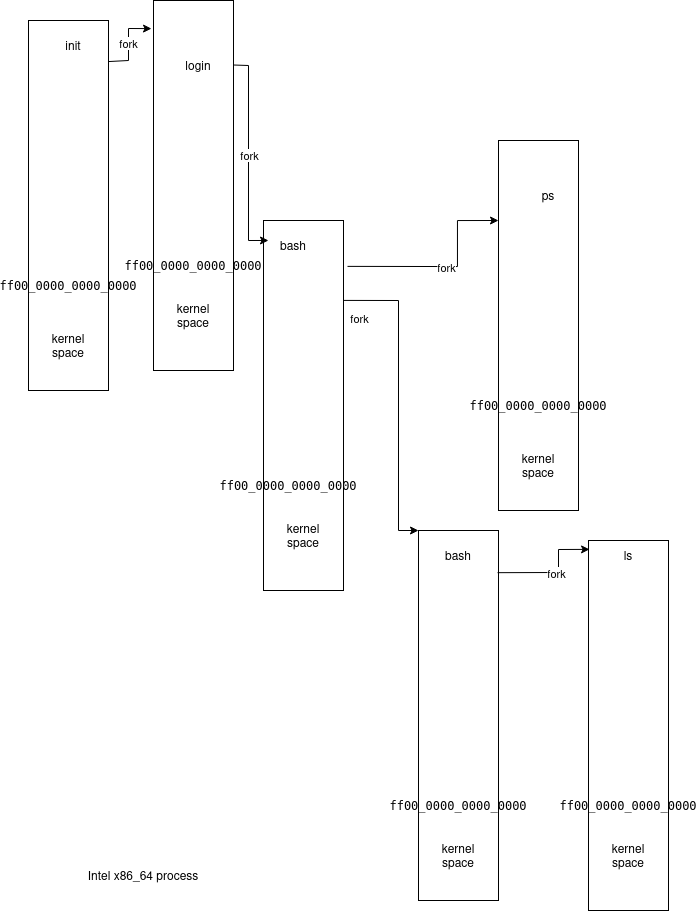
\includegraphics[width=10cm,height=13cm]{images/shell.png}
    \end{center}
    寫一隻shell其實非常簡單,主要是捉到user打的命令後,用fork跑出另一process
    (記住unix like是多人多工的然後在要這個child process用exec去執行這個
    外部程式例如ls, rm...等等。所以shell內部的運作大概是這樣的)
    \begin{enumerate}
    \item shell程式利用/dev/tty控制住鍵盤螢幕
    \item 打出prompt等待使用者輸入命令
    \item 捉到使用者輸入
    \item fork()一個新process
    \item exec()命令
    \item 執行完這個命令又回到shell
    \end{enumerate}
    在這邊您會看到unix like的執行一個程式都是藉由exec這個system call來執行的,
    這是作業系統提供使用者程式執行程式的機制。system call是user程式跟kernel
    溝通的管道。
    \\\\
    在以前MS DOS時代,一開機後會去執行command.com這隻程式就是shell。
    他就會跑出
    \begin{verbatim}
    C:\>
    \end{verbatim}
    等使用者輸入命令,這個C:就是提示符號(prompt),bourne shell通常prompt是\$,
    只不過這個dos shell功能相當的差,所以當時有個很有名的4DOS這個shell可以取代
    他。(4DOS這個shell其實拿了很多unix上shell的特性。當然跟真的unix shell還是
    不能比) 如果您只是用老鼠按一按一些icon,後來的MS-Windows時代,X的時代的
    command line shell就被圖形化的介面給取代了。不過執行另一個程式的機制還是一
    樣,還是要exec()。
    \\\\
    unix like 的系統的命令交談式的shell基本上除了能執行外部命令,主要他可以
    ''解釋''一些字串來執行,這些字串script的好處是可以設定一些環境。
    把多個外部命令集合起來完成一件工作。
    例如在Windows下我們也會設定TMPDIR這樣的目錄指到那個目錄去,有些windows程式
    會把執行中的一些暫時檔案放在這裡。unix like的shell scripts語法可以有if, 
    while, for loop等等,搭配一些外部命令,可以隨著環境不同時有不同的設定,
    使得一些日常工作維護更得心應手,比老舊的dos shell更為強大。
    \\\\
    sed, awk....,這些外部工具久而久之已經算是標準的unix系統必備的命
    令工具,就像winzip可能變成每個windows都會裝的工具。很多工具算是不成文的內定
    輔助shell programming工具了。所以真正說起來shell programming不單單是光
    懂shell的語法而已,而是要懂其他程式的選項,語法拉拉雜雜的一堆東西。
    \subsection{執行shell script與subshell}
    兩種方法
    \begin{itemize}
    \item 喚起新shell再執行shell scripts
    \item 在目前shell執行shell scripts
    \end{itemize}
    喚起另一個shell來執行的scripts在scripts檔頭最前面前要加
    \begin{verbatim}
      #! /bin/sh
      #! /bin/bash
    \end{verbatim}
    使用 sh 跟 bash 會有不一樣的行為,bash 會有比標準 sh 更多豐富的語法支援。
    \\\\
    第一種方法是在shell script 文字檔前指出shell scripts解讀的程式在那(也就是
    我們的shell)然後把文字檔的執行權限打開,照一般執行可執行檔方式執行或者叫
    一個shell來解釋文字檔test.sh。
    \begin{verbatim}
      $ test.sh
      $ /bin/sh test.sh
      $ ( . test.sh; )
      $ exec test.sh
      $ cmd1 | cmd2 | cmd3
    \end{verbatim}
    第二種方法是用命令''.''或者source執行。
    \begin{verbatim}
      $ . test.sh
      $ source test.sh
      $ { test.sh; }
      $ eval '. test.sh'
    \end{verbatim}
    差別在於一些設定只有在這個shell下的才算數,而喚起另一個shell就是另一個
    不相干的世界,
    也就是用第一種方法執行的script中變數的設定,不會影響到原來的shell變數。
    這個相當重要,其中很重要的是pipeline執行是喚起每個subshell來執行命令,
    然後把stnadard in standard out 串接,但是在各個subshell的變數是不互通的。
    ksh沒有source這個命令,所以最好不要用source。
    中括號( )表示用另一個subshell大括號,\{ \}表示用目前shell。例如
    \begin{verbatim}
      $ ( VAR='testvar'; )
      $ echo $VAR

      $ { VAR='testvar'; }
      $ echo $VAR
      testvar
    \end{verbatim}
    只有\{ \}內的VAR中的值被設定。其中用 . 的方法要很小心,
    不要在script裡面用
    \begin{verbatim}
      $ . test.sh arg1 arg2
    \end{verbatim}
    因為arg1 arg2會繼承呼叫這個script的arg1 arg2來,用 . 的方式最好是要執行
    的script只是一團script library不帶參數。
    另外如果 . test.sh執行,test.sh離開時,呼叫. test.sh的shell也跟著離開。

    \section{變數函數與模組化寫作}
    \subsection{變數使用}
    給變數值用
    \begin{verbatim}
      var="value"
      var='value'
      var=`command`
    \end{verbatim}
    要把值拿出來要加個錢符號\$
    \begin{verbatim}
      $ var="I am a gyoza"
      $ echo $var
      I am a gyoza
      $ var=`ls *`
      $ echo ${var}

      $ var='$var'
      $ echo $var
      $var
    \end{verbatim}
    以上要注意的是空格是有差別的還有引號的不同與作用。請往下看
    \subsection{引號quote}
    鍵盤上的double quote, single quote, backquote要弄清楚。
    \begin{itemize}
    \item backquote `command` 這個是命令取代,跟 \$(command)很像。
          所以常常看到var=`command或者var=\$(command),
          就是把command執行結果設給var。backquote會作反斜線的escape但
	  是\$(command)不會,所以如果有double scan變數時要小心。
    \item single quote 在' '內的文字通通保持原樣不做代換,有些保留符號在單引號
          內不再保留特殊意義。
    \item double quote 在" "內的文字\$ ` "三種意義會代換,其它的保持原樣
    \item escape char  在\verb=\=  後的單一字元也可以保持原樣
    \item 但是要escape ' ",就無法用反斜線,而是需要交互使用"跟',主要是shell
          的字串跟C一樣,是可以自動連結的,"string1"'string2' 就會變成
          string1string2,所以必須使用交互使用的"'"'"'來escape掉' 與 ",
          echo "'"'"'玩一玩。
    \end{itemize}
    \subsection{中括號的變數取代}
    加上括號\verb={}=是parameter的方法,
    \verb=${var}=是比較好的寫法,如果沒有要加其他字串可以用\$var就好。
    小心空格是有差的,他不像其他程式寫作,多空一個與少空一格是有差的。
    其他變數一些用法:
    \begin{itemize}
    \item \$\{var:-value\} 如果var有值了那麼就用原本的值,不然用value的值
    \item \$\{var:+value\} 如果var有值就用value的值
    \item \$\{var:?message\} var有值那麼就用原本的值,不然就印出message
      值到螢幕並且跳出。
    \item \$\{var:\%pattern\} 如果pattern與var後面的部份吻合,傳回剩下沒有
      吻合部份給var
    \item \$\{var:\#pattern\} 如果pattern與var前面的部份吻合,傳回剩下沒有
      吻合部份給var
    \item \$\{var/pattern/substitute\} 如果var有pattern吻合就代換成substitute
    \item \$\{\#var\} 這是字串長度,相當於strlen(var);
    \item \$\{var: offset:length\} 這是substring, \$\{var: -4:2\}
      表示從屁股第四個字元處拿回兩個字元。由於- 在前面是有用途的,所以要從屁股
      拿時,必須冒號後面空一格。
    \end{itemize}
    請看一個例子
    \begin{verbatim}
      # remote shell $RSH會等於/usr/bin/rsh  如果RSH當初沒有給值
      RSH=${RSH:-/usr/bin/rsh}

      # :+ 這種方式用在可有可無的option很好用
      # 以下面這個副程式為例子
      # 如果傳參數給他則VAR變成"-o 參數",沒有參數則VAR沒有值
      # $1 是第一個傳進來的參數  如果有值VAR就用"-o $1"
      func()
      {
          VAR=${1:+" -o $1"}
      }

      # :% 這種可以用在擷取字串的某部份
      # 例如  find 或者有的命令取回的結果往往是絕對路徑名
      # 但我們只想要最後面的那個檔案名時可以用這個來擷取
      # 不過傳統的bourne shell沒有% # pattern match,這只有在
      # ksh bash才有 最好不要用改用sed比較保險一點

      PRIV_HOST=fermion-priv
      PUB_HOST=${PRIV_HOST:%-priv}
      echo $PUB_HOST
      (PUB_HOST會等於fermion)

      # 代換也是  在新的Korn shell與Bourne Again Shell上才有
      
      BLOCK_DEVICE=/dev/vx/dsk/oracledg/vol_0
      RAW_DEVICE=${BLOCK_DEVICE/dsk/rdsk}
    \end{verbatim}

    \subsection{環境變數}
    普通的變數 如果Bourne shell, korn shell下用 \\\\
    \$ export var \\\\
    c shell, turbo c shell用 \\\\
    \$ setenv var \\\\
    則這個變數就變成一個環境變數。在C裡面的\\

    main(int argc, char **argv, char **envp)\\ 

    我們可以在shell裡設環境變數,而這個值是每個由這個shell fork出的程式,
    經由envp都看得到的。這個argv, envp指的都在virtual memory的下面stack
    往上長的開始處。
    所以shell也不過是一個"User space的C program",環境變數藏在C image user 
    space最下面,也可以從getenv這個library function call拿到。
    所以一般光設變數,沒有設環境變數沒有辦法把值告訴其它的程式。
    這邊要注意的是原本的Bourne shell的export沒有支援\\\\
    \$ export var=value\\\\
    的寫法,所以看到一些shell scripts為了portable起見都用\\\\
    \$ var=value \\
    \$ export var \\
    \subsection{一些內定變數}
    \begin{itemize}
    \item \$? 前一個命令執行完的status,
      0表示沒問題,在程式設計裡,0表示FALSE也表示No ERROR,所以程式的exit
      與return要處理好
    \item \$\# 表示傳給shell的arguments數量,這常跟\verb=set --=合用。
    \item \$0 這個shell命令名字
    \item \$1 \$2 \$3 ... function傳進來的參數arguments,
    \item \$@ 表示function 傳進來的所有arguments,如果加上double quote會等於
      "\$1" "\$2" "\$3"
    \item \$* 表示function 傳進來的所有arguments,如果加上double quote會等於
      "\$1 \$2 \$3"。 如果IFS有設值的話,例如 : ,那會是"\$1:\$2:\$3",所以使用
      for p in \$*; do echo \$p; done 跟 for p in "\$*"; do echo \$p; done
      的結果是不一樣的。
    \item \$\$ 表示目前的process ID
    \end{itemize}
    這邊\$@ \$*是不一樣的要小心double quote的不一樣,用*是會變成單一值的。
    \$?用在測試條件的判定是最常用的。
    \\\\
    shell一開始也會設定一些內定環境變數,這些環境變數會有一些程式自動會來讀取,
    例如mail程式用的MAIL,還有指明命令所在搜尋目錄的PATH等等。
    這些是寫bash, ksh, csh的C一開始寫在C程式內的。
    看環境變數用env這個命令,看變數用set命令就看得到不一樣結果。

    \section{函數與多檔模組化}
    函數的定義很直接就是
    \begin{verbatim}
func()
{
    cmd
    cmd
    ...
    return 0;
}
    \end{verbatim}
    傳值也是一樣的道理\$1 \$2 ...\$@ 等用法是一樣的。
    呼叫時就是
    \begin{verbatim}
func arg1 arg2 ...
    \end{verbatim}
    要注意的是變數是沒有像C一樣的有local variable,通通是global的。
    簡單的perl也是這樣。bash 有提供 local 修飾,但也不是傳統 sh 通用的。
    \\\\
    return 數字會變成\$?這個變數,return 字串沒有意義。在function內用echo
    會輸出到standard out。要作function執行後的判斷,可以用\$?或者讓他echo
    一些字串當成true。
    \subsection{模組化程式}
    function是最簡單的modulized寫作,再來就是多個模組檔當成shell lib檔。
    用了多個檔的問題跟C是一樣的就是變數怎樣在一個檔定義了,然後讓別的檔參照。
    通常export 成一個環境變數或者用eval這個內部命令執行一個個shell script使得
    這變數是大家都看得到的。

    \section{重要外部與內建命令}
    我們常用的ls, cp, sh....等等這些都是一個可執行檔,相對於一個外部可執行檔,
    shell有一些內建的命令藏在shell裡面,這些是built-in的內部命令是當初用C寫
    shell這隻程式時就寫在裡面的,像cd, export這就是。
    \\\\
    bash其實有很多以前的外部命令他都包含進來作成內部命令了,例如echo, getopts,
    不過為了程式可攜性,我們還是把他們稱為外部命令。這些內建命令可以用enable, 
    disable在bash內取消掉。不過別的sh, ksh或許就沒有了。要小心。
    \subsection{內建命令}
    比較重要且難一點的內建命令有
    \begin{itemize}
      \item : 假指令,甚麼都不作,等於CPU內的NOP指令。
      \item eval 大部分用來作兩次變數替換
      \item exec 執行某種命令並且替換掉目前shell(原本的執行不會替換掉shell)
      \item read 得到使用者從standard in(鍵盤)輸入
      \item set shell的精細設定,例如debug shell scripts
      \item test shell scripts的控制語法內的測試條件
      \item trap 接到某種訊號的處理
      \item shift arguments的處理
    \end{itemize}
    \subsubsection{ : magic numbers與註解}
    :是不做任何事的,在Unix中系統要執行程式會去檢查檔案前的字串叫
    magic number,古老的Bourne Shell的執行magic number是 : 而不是 \#!
    所以看到這種以:開頭的shell script可就要肅然起敬,同時:也有人拿來作註解用
    而不用\#的,主要是這可以拿來做大段落的comment,這特別要用單引號
    \begin{verbatim}
: << 'BLOCK_COMMENT'
blablabla
blablabla
alibuda
BLOCK_COMMENT
    \end{verbatim}
    這些老習慣的shell script可都是很厲害的。
    \subsubsection{eval與脫逃字元}
    eval可以拿來執行一個命令,不過他最常用的是拿來作兩次變數的代換,
    主要是每次執行一個shell
    命令他會先evaluate一次,看到有\$這個東西的就把值換一次把變數換掉,
    然後再執行一遍。這種double scan的方法對一些變數代換很有用,
    因為eval不是喚起另一個shell來執行,而是在本來這個shell內多evaluate一次,
    所以代換結果可以保留下來。
    例如如果我們要兩次代換
    \begin{verbatim}
      count=1
      var1=I
      var2=am
      var3=a
      var4=gyoza
      while [ $count -lt 5 ]; do 
         eval "echo \$var$count"
         let 'count=count + 1'
      done
    \end{verbatim}
    count可以一直變化1. 2. 3 ....要產生一個新變數var1 var2 var3....然後再對
    var1 var2取值。其中因為第一個var不想被運算,所以先用escape字元\verb=\=,
    然後第二次運算時才被解釋。
    那如果要三次以上變數代換在一行內解決呢? 想想看吧。要注意的是backguote跟
    \$(command)在double scan的不同,只有backquote會作反斜線\verb=\=的代換。
    \\\\
    eval主要還用來evaluate執行一個shell script檔,可以像C一樣寫成很多的
    模組shell script在同一個shell下run,則變數在此shell內通通有效。
    \begin{verbatim}
    $ eval ". foo.sh"
    \end{verbatim}
    不過如果變數太多,名字會打架。
    \subsubsection{exec}
    exec 會把''目前''的shell整個process拿掉,換成後面的命令,其實這就是用
    exec()這個system call置換掉子行程的意義是一樣的。
    最常看到是在~/.xinitrc這個scripts中置換掉成window manager。例如
    exec twm。
    所以如果你在shell中執行
    \begin{verbatim}
      exec cmd
    \end{verbatim}
    而cmd這個命令不存在就會回到login去,因為整個shell被換到cmd,但卻沒
    有cmd這個執行檔。
    所以執行程式的方法兩種是不一樣的
    \begin{verbatim}
      $ exec cmd
      $ cmd
    \end{verbatim}
    放在scripts的執行當然也不一樣。
    不過exec在script有另一個相當重要的用途就是跟file descriptor的連結,
    這個等下面再來討論。
    \subsubsection{read}
    \begin{verbatim}
    $ read input
    read from standard input
    $ echo $input
    read from standard input
    \end{verbatim}
    則會停在這邊等待鍵盤輸入,輸入字串變成\$input這個變數的值。
    \\\\
    其實read是等著從standard input拿東西進來,請記住是目前這個shell的standard
    input,所以像下面的作法是沒有辦法給變數值的
    \begin{verbatim}
    pipeline其實是叫sub shell執行每一道命令,此var是在另一個subshell中

    $ find . | read var

    用( )是喚起另一個subshell

    $ ( read var )
    \end{verbatim}
    \subsubsection{set}
    set通常是拿來設定這個shell的執行環境的。所以set跟環境變數中的值有很大關係,
    他後面的arguments會自動分到\$1 \$2 ....。比較重要的script會用到的大概
    \begin{itemize}
    \item set \verb=--= 正常看到-後面是option,現在不再是option
		而是一個命令參數。如-1 -2 ...這個可以變成一個參數。
    \item set -a 從這邊以後變數自動變成環境變數。
    \item set -f 不要解釋檔名的特殊字元例如wildcard *不再解釋為所有的意思了。
    \item set -x debug shell scripts
    \item set -o ignoreeof   一定要用exit離開shell,本來按Ctrl-D(eof)也可以
    \item set -o noclobber   關掉I/O導向不準overwrite檔案
    \item set -o notify      shell結束時報告background job的status
    \item set -o noglob      關掉wildcard字元解釋 如 * ? [ ]
    \item set +o 把-o的反向操作
    \item set -  關掉-v -x \verb=--=三種選項
    \end{itemize}
    set \verb=--= 或者set - 常常用在shell scripts裡面。其中set \verb=--=常用在
    set \verb=--= "val1 val2 val3",會變成\$1=val1 \$2=val2 \$3=val3。也就是
    \$*='val1 val2 val3'。如果後面沒有arguments,那就unset \$*。
    set -o 是很常用的例如set -o vi設定shell的操作方式用vi方法,
    取回上個命令就是按ESC再按k囉。 set -o emacs就是用 emacs 的方法 Ctrl-p 
    或上鍵。
    \subsubsection{test}
    test是控制語法中的測試條件,這個在下面討論。
    \subsubsection{trap}
    捉到某個signal時shell做的對應,
    \begin{verbatim}
    通式
    $ trap "command" signo
    其中signo是
    cyril@grill:~$ kill -l
 1) SIGHUP       2) SIGINT       3) SIGQUIT      4) SIGILL
 5) SIGTRAP      6) SIGABRT      7) SIGBUS       8) SIGFPE
 9) SIGKILL     10) SIGUSR1     11) SIGSEGV     12) SIGUSR2
13) SIGPIPE     14) SIGALRM     15) SIGTERM     17) SIGCHLD
18) SIGCONT     19) SIGSTOP     20) SIGTSTP     21) SIGTTIN
22) SIGTTOU     23) SIGURG      24) SIGXCPU     25) SIGXFSZ
26) SIGVTALRM   27) SIGPROF     28) SIGWINCH    29) SIGIO
30) SIGPWR      31) SIGSYS
    例如
    $ trap "" 2
    $ trap "rm $TMPFILE" EXIT 1 2 15
    \end{verbatim}
    如果""的command則表示shell不處理這個signal,
    2號就是INT通常就是按了Ctrl-C打斷shell script的執行,15就是
    TERM(process被kill了),再看難一點的例子
    \begin{verbatim}
trap_init()
{
        trap '  scriptcleanup
                [ "$SCRIPT_DISP" = ABORT ] && exit 100
                [ "$SCRIPT_DISP" = PASSED ]; exit $?' EXIT
        if [ -z "$__TC_INTERACTIVE" ]
        then
                for sig in HUP INT TERM; do
                        trap "  trap - HUP INT TERM;
                        echo 'Signaled - cleanup after script ...' >&2;
                        scriptcleanup $sig; kill -$sig $$; exit 101"  $sig
                done
        fi
        trap : PIPE
}
    \end{verbatim}
    這個例子的前面如果抓到EXIT這個signal就執行scriptclean到exit \$?的code,
    就是單quote內的東西,
    如果\$\_\_TC\_INTERACTIVE不是空字串,就執行下面的signal處理,
    如果是 trap - ,則表示回到最開始進入shell時的設定。
    最後如果是SIGPIPE(13號)就不做任何事(冒號:)
    那這有什麼好處呢,signal的處理相當於就是軟體中斷,在multiprocess時,
    可以可以成為兩個process間的彼此溝通。例如電動玩具的作法,通常一定有
    兩個process,一個負責鍵盤讀取,另一個負責一直重劃螢幕,所以就變成兩個
    process要互相溝通。有了trap,用shell都能寫文字電動玩具。

    \subsubsection{shift}
    shift是用來把進來的arguments移一個位移,
    shift n 移n個位移,
    shift可以拿來用超過10個以上的argrments,因為\$1 ... \$9只有9個而已。
    來看一個shell的queue list的append
    \begin{verbatim}
    # list_append list_name item ... - append items to a list
    list_append()
    {
        _list_a_name=$1; shift
        eval "set -- \${$_list_a_name} \$*"
        eval "$_list_a_name=\$*"
    }
    \end{verbatim}

    \subsection{外部命令}
    有些外部命令常用到
    \begin{itemize}
    \item basename 拿掉副檔名的處理
    \item echo 印出message的方法
    \item find 找檔案
    \item getopts 處理傳進來的arguments,跟C函式庫的getopt()很像
    \item xargs pipe時的命令執行與參數arguments的處理
    \end{itemize}
    另外sed awk會有專門介紹。
    \subsubsection{basename}
    捉出檔名副檔名工具。
    \begin{verbatim}
    $ basename foo.c .c
    \end{verbatim}
    則副檔名 .c 會被幹掉
    \begin{verbatim}
    $ basename /dira/dirb/dirc/foo.c
    \end{verbatim}
    則會剩下foo.c
    \begin{verbatim}
    $ dirname /dira/dirb/dirc/foo.c
    \end{verbatim}
    會抓出/dira/dirb/dirc
    \subsubsection{echo}
    echo是印出東西到螢幕的手段(也有print, printf可以用),
    這邊要講的是sh, ksh內的echo與bash的不一樣,所以設定有些不一樣。
    \begin{verbatim}
    echo -n  "messages"     不要換行(newline)
    echo -e  "messages\c"   解釋escape字元\c,等於-n用法
    echo -e  "\t messages"  tab在messages前
    \end{verbatim}
    傳統sh, ksh是沒有-n -e選項的,直接用echo就好。
    \begin{verbatim}
    echo "messages"     要換行(newline)
    echo "messages\c"   解釋escape字元\c 不要換行(newline)
    echo "\t messages"  tab在messages前
    \end{verbatim}
    使用-n -e可以用來處理binary的資料,最常用就是用hex,例如
    \begin{verbatim}
    echo -ne "\x1b[32malibuda\n"   印出綠色alibuda
    chs="\x80\x21\x20\x00\x0c\xfe\xff\xff"
    echo -ne $chs | dd if=stdin of=/dev/sdc seek=446 bs=1 count=8
    \end{verbatim}
    對/dev/sdc第1 partiton資料直接修改。
    \subsubsection{getopt}
    getopts其實是ksh, bash的內部命令,getopt才是真的外部命令。
    這很像C裡的getopt()。請看個例子
    \begin{verbatim}
    while getopts :vp:x:y:d:T:X:Y: c
    do
        case $c in
        v) 
                VERBOSE=yes
        ;;
        p)
                PLOT_TEMPLATE="$OPTARG"
        ;;
        x)
                X_AXIS="$OPTARG"
        ;;
        y)
                Y_AXIS="$OPTARG"
        ;;
        T)
                TITLE="$OPTARG"
        ;;
        X)
                X_LABEL="$OPTARG"
        ;;
        Y)
                Y_LABEL="$OPTARG"
        ;;
        ?)       
                echo "$PROGRAM_NAME Error: $0 : Unrecognized option" >&2; usage;
                exit 2;
        ;;
        esac
    done

    shift `expr $OPTIND - 1`

    if [ $# -ne 1 ]
    then
        echo "$PROGRAM_NAME: must specify a multi-column data file"
        usage
        exit 1
    else
        DATA_FILE=$1
    fi
    \end{verbatim}
    其中冒號:是說這個參數一定要有跟著的參數值,沒有冒號像v表示後面沒有帶著參
    數值, 例如最常看到-v是說程式執行時是verbose mode就是這樣。
    \$OPTARG就是跟在後面的 參數,getopts自動幫我處理好,並且一個一個的丟進
    \$OPTARG來。他也有\$OPTIND跟C library的用法很像。
 
    \subsubsection{find}
    尋找檔案用的程式命令,
    \begin{verbatim}
    find . -name "regex"
    find / -type d 找directory
                 f 找plain file
                 l 找symbolic link
                 p 找named pipe file
                 b 找block device
                 c 找char device
    find . -perm 755
    find / -user cyril
    gzip `find . \! -name '*.gz' -print`

    not ! 有的shell要加\ 因為!有特別意義,例如bash表示取回以前的命令。

    find -name -type -o -name
    \end{verbatim}
    在script中很多時候都是脫逃字元問題,常看到\verb=\=時都要想到這是脫逃字元。
    在script中 ()也有特別意義表示喚起另一個subshell來執行所以碰到()時也要用
    脫逃字元。或者合sed awk一起使用時也是一樣的道理。
    \subsubsection{xargs}
    xargs用來處理一些輸出結果要來當另一個輸入的arguments碰到的問題。
    例如
    \begin{verbatim}
      # find /usr/include/ -name "*.h" | xargs -n 2 diff
    \end{verbatim}
    -n2是指定有兩兩當成輸出變成diff的argumnets
    \begin{verbatim}
      # find /usr/include/ -name "*.h" | xargs grep '#ifdef'
    \end{verbatim}
    正常內定是輸出的一拖拉窟的結果,有用xargs時是一個一個餵給後面的命令
    \begin{verbatim}
      # find /usr/include/ -name "*.h" | xargs -i cp {} ~/include/
    \end{verbatim}
    -i 與 \{ \}可以把find的輸出的每一個當成cp的第一個argument,~/.就可以當成第
    二個argument。
    其實find裡面有-exec這個選項後面也可以用\{ \}表示一個一個餵給後面程式,而不是
    一拖拉庫的餵給後面程式。
    \begin{verbatim}
      # find /usr/include/ -name "*.h" -exec cp {} ~/include/
    \end{verbatim}

    \subsection{簡單數學}
    主要是拿來作counter的,有很多種方法,下面介紹三種,
    bash有個內建的let,
    例如
    \begin{verbatim}
let 'x = x + 1'
let 'x = x * 1'
    \end{verbatim}
    注意!!這邊等號右邊的x取值時不用加錢符號,而且在單quote內也可以有空格。
    ksh也有內建的,不過這不是每種shell都有的,
    比較保險的portable作法是用expr這個外部命令。
    請看例子
    \begin{verbatim}
 if [ "$KSH" ]
 then
        eval '
        add()
        {
                result=$((${1} + ${2}))
        }
        sub()
        {
                result=$(($1 - $2))
        }
        mul()
        {
                result=$(($1 * $2))
        }
        div()
        {
                result=$(($1 / $2))
        }
        inc()
        {
                eval "$1=\$((\${$1} + ${2:-1}))"
        }
        dec()
        {
                eval "$1=\$((\${$1} - ${2:-1}))"
        }
        '
else
        add()
        {
                result=`expr $1 + $2`
        }
        mul()
        {
                result=`expr $1 \* $2`
        }
        div()
        {
                result=`expr $1 / $2`
        }
        sub()
        {
                result=`expr $1 - $2`
        }
        inc()
        {
                eval "$1=\`expr \${$1} + ${2:-1}\`"
        }
        dec()
        {
                eval "$1=\`expr \${$1} - ${2:-1}\`"
        }
    \end{verbatim}
    這上面定義了一些副程式,可以在script裡面一樣像呼叫一般命令呼叫。
    \$((1+1))是一個subshell執行1+1並且傳回結果,下面例子讓我想起我的basic程式
    \begin{verbatim}
     i=0
     while [ $((i=$i+1)) -lt 10 ]; do echo $i; done
    \end{verbatim}
    不過\$(( ))這跟\$\{VAR\%value\}一樣只有ksh bash有, (( )) 在 bash
    中代表了數學 context ,裡面的 + - * / 還有 \verb=< >= == 都是像 c 一樣的
    數學運算。在if else 中也可以用。最好不要用在需要 portable 的shell程式上。
    副程式的position parameters \$1, \$2 ....跟平常script程式原則一樣。
    \\\\
    如果要更多的數學例如小數點的運算或者sin log等函數使用, 就用bc和awk吧。
    或者現在系統上一定都有 perl, python,也可以用
    \begin{verbatim}
    $ echo "$i $j" | awk '{print ($1 + $2) / 3.1415926}'
    $ echo "$i + $j / 3.1415926" | bc -l
    $ echo "" | awk '{print (i + j) / 3.1415926}' i=$i j=$j
    $ r=5; python -c "print('%.2f', (2 * 3.1415 * $r));"
    $ r=5; perl -e "print(2 * 3.1415 * $r);"
    \end{verbatim}
    ksh與bash都支援typeset,不過傳統的sh並不支援,bash還有declare這個內部命令,
    這兩個都是拿來定義這個變數是甚麼性質的很像C的宣告。不過為了portable能不用
    就不要用,還是用最基本的sh就好,如果真的要寫得很複雜就用perl, python吧,
    如果非常的嚴謹就用C囉。
    \begin{verbatim}
      $ typeset -i int_var
      $ declare -r constant
    \end{verbatim}
    int\_var被設成整數,如果給字串則int\_var的值會是0。如果用-r 
    則constant的值從現在起不能再被改了。

    \section{File descriptor與I/O導向}
    一個程式最基本的會自動開啟三個檔,操作時相對應的代號就是file descriptor,
    其實也就是跟作業系統開檔每次要到的file descriptor,是per process的
    \begin{itemize}
    \item 0  standard input   通常就是鍵盤
    \item 1  standard output  通常就是螢幕 buffer I/O
    \item 2  standard error   通常就是螢幕
    \end{itemize}
    stderr 跟 stdout 都是輸出到螢幕,差別就是 stdout 是 buffer I/O ,他會等到
    所有字元都準備好了,才輸出到螢幕, stderr 不是,是馬上就輸出到螢幕,因此
    在練習多工程式中,錯誤訊息都是要馬上丟出螢幕的。
    以前很常用的 pipe
    \begin{verbatim}
    p1 | p2 | p3 ...
    \end{verbatim}
    就是把每個 process 的 stdout 串成下一個的 stdin
    \\\\
    我們可以用I/O導向
    \begin{verbatim}
      $ cat file1 > file2
      $ pgr1 2> error
      $ dirs 2>&1 > /dev/null
      $ dirs > /dev/null 2>&1
    \end{verbatim}
    來將結果導向。導向跟pipe是不太一樣的,I/O導向是dup2()這個system call,
    而用pipe用的是pipe(2),所以導向的順序是重要的,如果是先導向/dev/null的表示
    先duplicate一個file descriptor跟/dev/null一樣,再
    執行dirs時所產生的standard error丟到standard out再到黑洞/dev/null去,
    就是甚麼也看不到。所以dirs \verb=2>&1 >= /dev/null跟 
    dirs \verb=> /dev/null 2>&1= 是不一樣的。
    \\\\
    既然是 process 的 fd,所以他其實最真實的規則是
    \begin{verbatim}
    (process 1) 1> (process 2)
    (process 1) 0< (process 2)
    \end{verbatim}
    只是 1 跟 0 省略不寫而已。 而後面接檔案的意思只是有個看不見的 process
    幫你開檔,產生的 stdin, stdout 。因此
    \begin{verbatim}
      $ cat file1 > file2
    \end{verbatim}
    是說 cat 這個程式把 file1 的內容印出到 stdout,然後把他丟給一個不知名的
    process 開了 file2 的 stdin 去,然後這個不知名的 process 把他的 stdin
    內容填入到 files 去。所以只是 bash 特別給的語法給使用者方便,這個語法通
    用有
    \begin{verbatim}
    p1 m>  file  p1 重新導向fd m 並且先把檔案虧空
    p1 m>> file  p1 把結果導向fd m並且append到檔案後
    p1 m<  file  p1 重新導向開file 的 process 的 stdout 到p1 fd m
    p1 m>&n      p1 把p1 process 的 fd m 丟給file descriptor n
    p1 m<&n      p1 從file descriptor n 拿東西給p1 process 的 fd m
    p1 m>&-      p1 close process fd m
    p1 m<<text   p1 把 fd m 導向,直到讀到下個text為止,請看 Here 文件章節。
    p1 m< <(p2)  p1 把 process 2 的 stdout 變成p1 的 fd m
    p1 m&>       bash 特有的語法 &> file 表示 > file 2>&1,這跟 >& 顛倒
    \end{verbatim}
    前面的 m 很多時候在 stdin, stdout 都是省略的,
    要注意的是有些後面只能接檔案,有的接file descriptor,還有
    接file descriptor時不能有空格。而
    \begin{verbatim}
    dirs > /dev/null 2>&1
    \end{verbatim}
    dirs 這個執行的 stdout 變成開 /dev/null 程式的 stdin,那後面的
    \verb=2>&1= 指的 是 dirs 呢?還是開 /dev/null 的 process 呢?
    以結果論來說是 dirs 這個 process 的 2 變成 dirs 的 1.
    \\\\
    exec 最常用在與file descriptor 的關聯這裡
    \begin{verbatim}
      $ exec 3> LOGFILE
    \end{verbatim}
    exec 在前面說到是執行某個程式,整個跳到那裡去,但在 shell 裡面就是自己
    這個 bash ,所以 exec 3 變成把自己 bash 的 fd 3,連到不知名程式開檔
    LOGFILE 的 stdin ,然後一樣道理而已。
    \begin{verbatim}
      $ exec 2>&-
      $ exec < infile
    \end{verbatim}
    因此其中各意義分別為把standard err關掉。 把目前shell的standard input變成
    infile,然後要導到fd 必須用 \verb=>&=。以下例子為把 fd 10 跟 newfile
    關聯起來
    \begin{verbatim}
      $ exec 10<> newfile
      $ ls /proc/$$/fd
      $ echo something >&10
      $ cat newfile
      $ read -r line <&10
      $ echo $line
      $ exec 10>&-
    \end{verbatim}
    注意file descriptor 1,2,3與導向符號的空格。空格的格式不是亂空的。還有
    fd 不等於 newfile,他是 system call 的 open/read/write 的 fd,一旦
    建立,只是當時狀態的 fd buffer,所以後來用別種方式加減 newfile,是
    無法影響 fd 10 的狀態的。
    \\\\
    而因此有的命令像 read 是從 bash 這個 process 的 stdin 讀東西進來
    \begin{verbatim}
    read -r line < myfile
    read -r line <&4
    \end{verbatim}
    很多工具程式都會提供從 stdin 輸入,從stdout 輸出的轉向功能語法,
    最常用的就是用 hypen - 表示 stdin,或者使用 Linux 中的 /dev/stdin
    /dev/stdout 表示目前 process 的 stdin stdout 的檔案。
    \begin{verbatim}
    cat - << file
    cat my.tar.gz | tar zxvf - myfile
    \end{verbatim}
    而
    \begin{verbatim}
    while read -r line; do echo $line done< <(process)
    \end{verbatim}
    這個重要意義就是後面 process 的 stdout 與前面 while do done 的 shell
    process stdin 的連結,用 () 執行程式在以前說過是在另外個 shell 呼叫這個
    程式。這很重要的是如果process 輸出是一行一行的,那 while read 也是一行
    一行讀進來,這在字串中避開含有空白做為分隔 dlimiter (IFS) 是很有用的技巧。
    如果是
    \begin{verbatim}
    while read -r line; do echo $line done 10< <(cat file | grep 'we want')
    \end{verbatim}
    就是讀進 while; done 的 fd 10,但當我們故意用
    \begin{verbatim}
    $ read -r line 100<& <(ls)
    bash: /dev/fd/62: ambiguous redirect
    \end{verbatim}
    出現 error ,表示 <(ls) 其實是被 expand 成 /dev/fd/62 這個神奇檔案。所以
    語法錯誤。這個 <(process) 語法主要是找最後一個有空的 fd 變得很重要,在 C
    程式中也是一樣,man dup 時可以看到他很強調這點,在 Linux 中,一個
    process 的有空的 fd 可以從
    \begin{verbatim}
    /proc/$$/fd
    /proc/self/fd
    \end{verbatim}
    下面看到,但只有 Linux 提供這個 /proc 檔,所以為了程式可攜性,在BSD, 
    SystemV AIX, Solaris ... 能跑,還有建立這種有 ID 的物件,都不要忘了多工
    搶資源的情況,一定要透過系統幫你做 atomic 運算,確保這個 ID 是獨一無二
    ,因此 bash 提供了
    \begin{verbatim}
    $ exec {var}>hellofile
    $ echo ${var}
    \end{verbatim}
    表示由 bash 幫你搶了一個關聯 hellofile 確保獨一無二的 fd 到 var 這個變
    數上。
    \\\\
    這個還有一個古怪的地方,正常講我們應該用
    \begin{verbatim}
    var=15
    exec ${var}>hellofile
    \end{verbatim}
    怎麼會少了錢符號?原來我們在使用變數來做 fd 也要小心,要用單引號把
    > 先框起來,做 eval var 那個變數擴展成數字先,才知道這是要做導向語法
    \begin{verbatim}
    eval exec ${var}'>'hellofile
    \end{verbatim}
    由於單引號的奇怪語法很彆扭,所以 bash 給了一個這語法同時解決上面三個問題
    。這個語法 ksh 早在 2006 就有, bash 要到 4.1 版以後才有,目前是
    KornShell 93r+, Bash 4.1α+, Zsh 4.3.4+ 以上才有。
    但這語法不是 POSIX 標準的,以新 2017 POSIX 標準來看,這還是不 portable
    的。

    \subsection{Here 文件}
    導向符號有個 Here 文件型的導向,
    \begin{verbatim}
    (process1)m<<XXX > file1
    alibuda
    2nd line
    asaburu
XXX
    \end{verbatim}
    表示兩個XXX中間夾住的文字都變成 process 1 的 stdin (m是0可不寫),然後導
    向 file1, 這有兩個好處,一個就是大片的多行文字定義可以用這方便處理,二
    就是大片文字等於是多行註解。
    \begin{verbatim}
:<<COMMENT
This is comment
comment multiple lines
COMMENT
    \end{verbatim}
    記得 : 是不做事,這樣就不用一個一個放 \# 在每行前面。
    \\\\
    自動ftp的 scripts 的例子,
    \begin{verbatim}
#!/bin/ksh
# A script to automate FTP transfer

HOST=ftp
USER=user
PASSWORD=password
FILENAME_PATTERN=remote_files
REMOTE_DIR=/usr/doc
LOCAL_DIR=/usr/local
# -i = non-interactive, -n = disable auto-login

ftp -i -n <<HERE
     open $HOST
     user $USER $PASSWORD
     cd $REMOTE_DIR
     lcd $LOCAL_DIR
     mget $FILENAME_PATTERN
     close
     bye
HERE
    \end{verbatim}
    注意\verb=<<=的用法,ftp的input會一直讀到HERE為止,open, user, cd, mget
    都是ftp中的命令。不過也可以把
    這些ftp命令寫成一個檔案然後ftp \verb=<= 檔案也行。
    \subsection{embedded其他script與資料檔}
    在上面的ftp的例子,我們可以看到 ftp 的命令可以嵌在shell script 裡面,
    同樣的perl script或者其他可以從 stdin 獲取資料的命令也可以嵌在 shell
    script裡面,只要善用\verb=<<=就好。
    請看例子:
    \begin{verbatim}
    while read column1 column2 column3
    do
            echo $column1 $column2 $column3
    done <<__ENDDATA__
    99      98 3.5
    300     298 4.9
    498     493 5.9
    699     698 7.6
    900     748 9.0
    1200    703 9.6
    1500    651 10.4
    1698    627 10.8
    __ENDDATA__
    \end{verbatim}
    while do done;裡面的read要從standard in讀,我們把他從standard in導到讀到
    \verb=__ENDDATA__=所以下面的資料就分別讀進column1 column2 column3。
    再看一個perl的內堪例子
    \begin{verbatim}
#! /bin/sh

    perl -x - $* <<'End-of-Perl-Script'
#!perl
        #
        # given absolute or relative pathnames, create symlinks from the
        # destination directory back to the source file(s) using relative
        # pathnames
        #
         
        if (@ARGV < 2) {
                print STDERR "must specify at least two files\n";
                exit 3;                                          
        }
        @srcfiles = @ARGV[0 .. @ARGV - 2];
        $targ = $ARGV[@ARGV - 1];

        if ($targ !~ m,/,) {
                $targ = "./$targ";
End-of-Perl-Script
    \end{verbatim}
    從這邊可以把perl用-x叫出來解釋perl的語法。

    \subsection{導向的用途}
    多工的 process 間資訊傳遞都是高級程式的重點,剛剛用的 file descriptor,
    其實就是多工 multiplexing 的最基本方法之一。可以從 parent process
    fork 出去的 child 連回 parent 來,兩邊互相送東西達成通訊功能。
    這在寫 shell 多工甚至一般 C 語言的多工都是一樣的道理。所以用 shell 是
    能寫電動玩具的,只要能一邊畫畫面,一邊接收按鍵,一邊處理運算這三個多工
    process 能溝通,就是一個標準的電玩程式。
    \\\\
    這種 file I/O 的多工,最基本的就是 pipe,某個 process stdout 變成另外
    process 的 stdin,這也可以用 mkfifo 建立一個有 in 跟 out 的特殊 fifo
    檔案,這也稱為 named pipe
    \begin{verbatim}
$ mkfifo inout
$ echo 'fifo in' > inout &
[1] 1763084
$ cat inout
fifo inout
    \end{verbatim}
    如果 inout 這個檔案裡面是空的,則一個 cat (read) 會 block 等在那裡直到
    inout 這個檔有內容進來。
    \\\\
    在一般使用上,可能最重要的多工是 terminal 的畫圖,例如 wget, curl
    下載檔案的 progress bar,這種一邊做某件事,一邊處理畫面都是多工應用
    ,即使是系統軟體在做長時間解檔,網路作業等跟 device 等待有關的程式
    也都會用到,這其實用 shell 就輕易的做到了。

    \section{流程控制與測試條件}
    \subsection{測試條件}
    在Bourne shell的內部命令裡面有測試條件的語法test給if while用
    \begin{verbatim}
    test condition
    或者 
    [ condition ]
    \end{verbatim}
    這個 condition 是process 程式丟出來的 status \$?,如果是 0 ,就是
    true,如果是非 0 就是 false。 為了與autoconf不要混淆,programmer
    比較喜歡用 test 不用中括號condition的方法。括號的用法請注意要有空格。
    例如
    \begin{verbatim}
    檔案測試條件
    test -f /etc/file      檔案是個一般檔案不是其他特殊檔案嗎
    [ -e file ]            檔案存在嗎
    [ -d /etc/ ]           目錄存在嗎
    [ -s file ]            檔案大小大於0嗎
    [ -r file ]            檔案可讀嗎

    字串測試條件
    [ "$string" ]          string有東西就返回true
    [ -n "$string" ]       string有東西(non-zero)返回true
    [ -z "$string" ]       string沒東西(zero)返回true
    [ "$s1"  = "$s2" ]     s1 等於 s2時返回true
    [ "$s1" != "$s2" ]     s1 不等於 s2時返回true

    數值條件  小心有多個-喔
    [ $num1 -eq $num2 ]    num1相等    num2 為true   
    [ $num1 -ne $num2 ]        不等    num2 為true
    [ $num1 -lt $num2 ]        小於    num2 為true
    [ $num1 -ge $num2 ]        大於等於num2 為true
    \end{verbatim}
    \begin{verbatim}
    多重條件
    [ ! -f "testfile" -o ! -r "testfile" ]
    [ test condition -o test condition ]
    !               表示not
    -a		    表示and
    -o		    表示or
    \end{verbatim}
    通常比較常用的又有portable的就是上面一些用法。bash 又給了特別的數學
    ((  )) 與字串 \verb=[[  ]]= 測試方法,在(( )) 中可以用 + - * /
    \verb/< > == && ||/ 等 c 語言的判斷符號,而且變數也不用\verb=$=符號,
    \verb=[[ ]]= 除了也可以用 == , != 外,還可以用 regex \verb/=~/,
    而且作用也不分別字串或數字,算是很方便。
    或者能用 if \verb=[[ ]]= -o \verb=[[ ]]= 這種寫法。
    但也是如果程式要能在標準的 sh 上跑,也是能不用就不用,否則還蠻好用的。
    美觀上來說用中括號condition比較好看,很多人為了 autoconf 的語法 portable 
    起見, 盡量用 test 的寫法。測試的結果當然放在\verb=$?=中,0 表示成功,
    其他值表示失敗。
    \\\\
    在shell script中也有可能看到有人用
    \begin{verbatim}
    if [ "x$VAR" = "xvalue" ]; then .....
    \end{verbatim}
    來作\$VAR是否是空的測試,尤其你如果先測試是否為空字串,
    再測試是那個值要做什麼,這樣就會作兩次測試划不來,用這樣作比較經濟。
    \\\\
    另外這跟perl字串與數值測試容易混淆,他跟perl剛好相反,而且perl沒有多-
    \begin{verbatim}
    perl語法
    if ($str1 eq $str2)
    if ($num1 == $num2)
    \end{verbatim}
    最後有個大比較,會一起列出shell perl c的差異來。(人老了記不住,我是這樣記
    ,以perl為基準eq是字,所以前後是string,==是符號所以前後是number,
    bourne shell是怪胎,剛好顛倒,eq還要加個-符號。==要少一個=)
    \begin{verbatim}
    C語法
    if (!strcmp(string1, string2))
    if (num1 == num2)
    \end{verbatim}

    \subsection{if 條件判斷}
    if test;then cmd1; elif test; cmd2; else cmd3 fi
    \begin{verbatim}
      if test
      then
        cmd1
        ...
      elif test
        cmd2
        ...
      else
        cmd3
        ...
      fi
    \end{verbatim}
    同樣注意寫成一行時的分號位置。尤其在寫Makefile時會用到。
    另外他的else if 是 elif, 跟 C 的 else if 不一樣。
    \\\\
    另外有種簡單的if用法
    \begin{verbatim}
    [ "$VERBOSE" ] && echo 'everything'  && 表示傳回true時執行&&後面動作
    [ "$VERBOSE" ] || echo 'nothing'     || 表示傳回false時執行||後面動作
    \end{verbatim}
    其實這就是
    \begin{verbatim}
    process 1 && proess 2
    process 1 || proess 2
    \end{verbatim}
    如果多個串接
    \begin{verbatim}
    process && process 2 || process 3
    例如
    echo 1 | grep 2 >/dev/null && echo haha || echo ahah
    \end{verbatim}
    則有 if else 的作用
    \\\\
    這邊有點要注意
    \begin{verbatim}
    [ "$var" ]
    如果是空字串傳回false 這其實很像
    [ -n "$var" ]
    -z 是如果是空字串傳回 true
    [ -z "$var" ] 
    \end{verbatim}
    這用在兩個以上 condition 連接有 not 的情況,不然光用 
    \begin{verbatim}
    [ ! "$v1" -o "$2" ]
    \end{verbatim}
    會分不清是先 not 還是 not 作用在整個有 -o 的情況。
    \\\\
    condition 由於是根據程式執行結果,但有的時候例如 find 這個程式,
    找不到檔案並不意味著執行失敗,只是找不到而已,所以找不到回傳的 \$?
    還是 0,這並無法幫我們做判斷,但有的命令成功了會在standard out 印出
    一堆字串,我們可以利用這樣的行為來作判斷,例如
    \begin{verbatim}
    if find . -name alibuda; then
        echo "I find it"
    fi
    \end{verbatim}
    是不行的,而要用
    \begin{verbatim}
      [ "$(find . -name gyoza.txt)" ] && echo "I Find It !!!"
    \end{verbatim}
    用\$(cmd) 很像用`cmd`,差別就是會不會做反斜線的替代escape,如果找到了,
    會印出這個檔案來所以雙引號裡面" "有值,中括號\[ \]就還回true囉。如果沒有
    雙引號,如果只有一個字串則會當成字串永遠為true,所以
    \begin{verbatim}
    $ [ 1 ]
    $ echo $?
    0
    $ [ 0 ]
    $ echo $?
    0
    \end{verbatim}
    如果有兩個以上,則shell把find丟出來的字串又當成命令,想去執行他,就發生
    錯誤了。
    \subsection{for loop}
    for var in \$list; do cmd1; cmd2; done
    \begin{verbatim}
      for var in $somelist
      do
        cmd1
        cmd2
      done
    \end{verbatim}
    注意寫成一行時的分號位置。尤其在寫Makefile時會用到。
    list是shell裡常用的一種方法,就只是很多小單位用空格或tab分開的資料就是。
    例如
    \begin{verbatim}
      ME="I am a gyoza"
    \end{verbatim}
    ME就是一個list(bash的man page用list表示一堆commnands,
    把word表示這裡的list,有的書或者ksh, sh的man page又不一樣。
    所以我很不喜歡去定義這些名詞,有時候爭論這些沒有意義
    捉到key point比較重要)for 敘述可以一次把一個元素餵給前面的var
    \begin{verbatim}
      for ELEMENT in $ME; do
        echo $ELEMENT
      done
    \end{verbatim}
    就會出現
    \begin{verbatim}
      I
      am
      a
      gyoza
    \end{verbatim}
    注意錢符號與設定變數使用變數的差異。
    \\\\
    bash 特別有像 C 的 for loop,所以要用(( )) 的方法。
    \\\\
    for (( i = 0 ; i < 10; i++)) ; do cmd1; cmd2; done
    \subsection{while loop}
    while test ; do cmd1; cmd2; done
    \begin{verbatim}
      while test;
      do
        cmd1
        cmd2
      done
    \end{verbatim}
    同樣注意寫成一行時的分號位置。尤其在寫Makefile時會用到。

    \subsection{case switch}
    \verb=case $var in *)cmd1; cmd2 ;; xx?)cmd3; cmd4 ;; esac=
    \begin{verbatim}
      case $string in 
           *) cmd1; cmd2
           ;;
           xx?)
              cmd3
              cmd4
           ;;
      esac
      case $answer in
           [Yy])
              echo 'yes'
           ;;
           [Nn])
              echo 'no'
           ;;
      esac
    \end{verbatim}
    case switch的用法,不像C的是整數的case switch而是可以有字串的喔,
    其中符合的字串條件用globbing的方式,也就是wildcard *, ?, \verb=[ ]=
    ,有的書上寫regular express是錯誤的。注意用一行寫出的方法。

    \section{bash 特殊資料型態}
    除了 (( )) 與 \verb=[[ ]]=的特殊用法外,
    一般程式語言很常用的 array 與 hash,原本 shell 是沒有的,就只是基本的
    字串用空白鍵分開的 list 而已。bash 提供 index array,他的literal
    \begin{verbatim}
    declare -a a

    a[0]='first'
    a[1]=2
    a=('first' 2)
    echo ${a[0]}

    for v in "${a[@]}"; do echo $v; done
    first
    2
    for v in "${a[*]}"; do echo $v; done
    first 2
    unset a
    \end{verbatim}
    帶有key 的 hash array
    \begin{verbatim}
    declare -A h

    h['key0']='value0'
    h['key1']=2
    echo ${h['key0']}

    for v in "${h[@]}"; do echo $v; done
    value0
    2
    for v in "${h[*]}"; do echo $v; done
    value0 2
    unset h
    \end{verbatim}
    使用@與*跟之前的 shell 變數一樣,用double quote時會有不同,*會變只有單一
    值,@會變成很多值。所以要用二維陣列,必須用*
    \begin{verbatim}
    twod=("${a[*]}" "${h[*]}")
    echo ${twod[0]}
    echo ${twod[1]}
    \end{verbatim}
    同樣如果是要在 portable 的機器aix, solaris, ...上跑的話,儘量用最原始的
    sh,這種array, hash 就最好不用。

    \section{結語}
    一般標準用shell是Bourne Shell後來延伸出Korn Shell,很多老一輩的工程師
    還比較喜歡用korn shell寫scripts。第一次碰到令人讚嘆的 sh script 就是
    老工程師用 ksh 寫的 testing script, 另外還有BSD的C shell,
    c shell 也造成一股風潮,尤其在很多system admin,這是因為在 1990 年代中
    Sun 的機器實在是賣的很好,在美國公司內的 admin 很會寫 csh 的 script,
    即使在台灣我做過 IC chip 的testing, testing 機器與教我的人也是 csh,
    所以大概以現在2017年,在 50 ~ 60 歲左右的人,很大部份用 c shell。
    我在幾家大公司中的 default shell 都是 csh, 後來 tcsh 加進很多不錯的特點。
    一直到現在,我們新進人員 default shell 還是 csh, tcsh,相關工具也一定有
    c shell 的 script,只是後來 Linux 大行其道,bash 慢慢聲勢浩大。以前剛進
    公司,配的是 Solaris 機器,後來只剩 Linux 機器,最後只給 laptop,遠端用
    Linux VM,自己去要一個 Linux VM 來用。
    Bourne Again Shell 把大家有的沒的特點拉拉紮紮放在一起。拜GNU/Linux之賜
    年輕一代的工程師很多喜歡 bash,不過要注意 portable 的 shell scripts 寫作。
    (只是我看其他unix like系統大概也都死的死逃的逃,bash也算蠻通用的了)
    sh, ksh bash是同一家族的,這幾個語法比較接近,不像tcsh csh是另一家族,
    差很多。

\chapter{Regular Express}
    \section{簡介-RE與glob}
    regular express是一種表示方法,用一些特殊的字元來表示一些電腦裡的特殊意
    義,並且做為尋找的一種樣式比對 \verb=(pattern match)=。
    在MS dos/windows 中也有相當的字元,例如 * 代表所有字所以你用del *.* 就可以砍
    掉所有檔案,* 就叫 wildcard 字元。不過這在 shell 中的處理只是叫做 globbing
    並不是regular express。其實這當然是從Unix學去的,UNIX上的regular 
    express 更強大,而且適用於很多Unix 軟體裡面,像grep, sed, awk, vi, emacs
    perl...等等,可以說 regular express 就是使用 UNIX 的靈魂。
    不過要來學unix請先把DOS那套不general東西給忘了。
    \\\\
    C程式裡面處理regular express如果是POSIX的系統則用 regcomp() regexec(), 
    System V的有regcomp(), regex(),BSD系統有re\_comp(), re\_exec()。
    \\\\
    在shell中的路徑pattern match叫globbing,shell 路徑是不認得 RE 的
    通常用於路徑名的 ? * \verb=[]= 的比對,對應用\verb=fnmatch()=來處理。
    不過這不是要談的重點,只是以後進階用C寫程式時可以想到用甚麼 function call。
    \\\\
    通常很多使用regular express的時後會用一對//夾住。
    \begin{verbatim}
      /reg express/
    \end{verbatim}
    來表示找到合乎reg express條件的字串。perl裡面說其實是
    \begin{verbatim}
      m//
      s///
    \end{verbatim}
    m表示match,s表是substitude,不過m可以省略不寫就變成//了
    通常用法是m//命令,s///命令。命令常看到的有
    \begin{itemize}
    \item p       -\verb=>= print   通常也不用寫
    \item d       -\verb=>= delete  這通常是跟在m命令後  符合的就砍掉
    \item c       -\verb=>= confirm 通常用在s命令, 詢問是不是真要取代
    \item g       -\verb=>= global  通通換,因為match到時內定只有第一個符合的有效
    \item i       -\verb=>= ignore  不管大小寫
    \item 1,2,3...-\verb=>= 表示搜尋取代的第一個,第二個,第三個....等等
    \end{itemize}
    不過也不一定,像grep命令就沒有,用雙引號就可以了。
    anyway,只是很多都是這樣表示。
    \section{字元處理}
    由單一的字元特殊符號表示一行中的特殊位置與連續性就可以組合成千變萬化的字串。
    \subsection{基本字元表示}
    字元,就是單一一個英文字母的處理。先來個基本的字元
    \begin{itemize}
    \item .   代表任意"一個"字元除了換行newline字元。不過記住awk可以match換行。
    \item ?   代表"前面"字元出現0次或1次
    \item +   代表"前面"字元出現1次以上 1 2 3 4 ... 不出現return false 
    \item *   代表"前面"字元出現0次以上 0 1 2 3 ...
    \end{itemize}
    這邊初學者比較常犯的錯誤是在shell下的wildcard * 的習慣,以為只要給個*
    就代表所有字元,其實是 ? + * 都要前面搭配 . 來使用才能代表任意字元。
    \begin{itemize}
    \item \verb=^=   代表行首
    \item \$   代表行尾
    \item \verb=\=   脫逃字元(escape)取消特定字元的涵義用的
    \end{itemize}
    這邊比較要注意的是字在行首起頭的\verb=^=,行尾的\$,與在行中的case分屬不同
    的regular express,小心有的程式會把這四種當成不同的regular express,
    這會不一樣喔。
    例如
    \begin{verbatim}
    beg                    ->  /^beg$/   才吻合
    beg your pardon        ->  /^beg/   才吻合
    I beg your pardon      ->  /beg/   才吻合
    I beg                  ->  /beg$/   才吻合
    \end{verbatim}
    不過有的不會。這種狀況也很討厭,在新的軟體如perl等就有很好的處理方式了。
    \\\\
    有的程式是以行做運算單位,有的如javascript卻還能以單一字串做運算單位。
    所以有的字元的含意會有多出來的意義。這要仔細的看各個軟體工具的說明。
    另外就是換行字元與空字元的使用再一些軟體使用情況不同,這也要小心。
    \begin{itemize}
        \item /\verb=^#=/      有\verb=#=在一行的第一字元時  就還回TRUE
	\item /\verb=^=bag/    bag在行首的行
	\item /bag\$/    bag結尾的行
	\item /bag/     bag在中間的行  不過有的程式處理沒有這麼嚴格像sed
	\item /b.g/     表示bag beg bug都行 
	\item /b\verb=\=.g/    表示b.g
	\item /\verb=^=..g/    表示行首bag beg bug xxg都符合 但一定要三個字母
	\item /\verb=^=.*g/    表示行首有任何字元的然後有個g的都可以還回true
	\item /beg*/    be, beg, begg, beggg, .......    
	\item /beg+/    beg, begg, beggg, begggg, ......
	\item / */      空白字元也行
	\item /\verb=^$=/    代表空白行 
    \end{itemize}
	\subsection{字元處理 - 括號與範圍表示}
	\begin{itemize}
	\item \verb=[ ]=       \verb=[]=內的任一"單一字元"符合就還回TRUE
	\item \verb=[^ ]=     \verb=[]=的反效果 不含\verb=[]=內的任一單一字元
			還回true,所以這邊\verb=^=在\verb=[]=內有不同的意義,
                        這個常用在收集完全沒有某些字元的長字串上。
	\item \verb=[0-9a-zA-Z]=    -號在\verb=[]=內可以表示一段範圍不用打到手酸死,
			所以如果要表示-號必須放在第一或最後字元
	\item \verb=w{n,m}=   連續字元出現表示法\\
		       比用 /.../好用,
                       跟{\LaTeX}中的table的用法很像,表示有"連續"符合
		       w字元出現''連續'' n次到m次 \\都會還回TRUE
	\item \verb=0{3,}=    0至少出現3次 \verb=->= /xxxx000xxxxxx/
	\end{itemize}
	在字串下\verb={} ()=是表示真的這些字元的,不像\verb=[ ]=會被regular
	express當成一種運算,所以不要忘了用脫逃字元 變成\verb=\{ \} \( \)=。
    \section{字串處理 - 不同括號表示}
	一些字串的處理上
	\begin{itemize}
	\item \verb=( )=	Group operator
	\item \verb=(str1|str2|str3)=  str1或者str2或者str3\\
			\verb=()= 與 \verb=|=是extend的regular expression
			只有一些軟體如egrep才有支援。所以在用軟體的regex
			時必須知道他能處理的regex能力。
	\item \verb=&=  表示s///中前面找到的字串
	\item \verb=\1 \2 \3= ... 代表s///中前面用括號\verb=\(\)=括起來的字串,
			這通常也是找到的字串,不過\verb=&=只有一個,
			用 \verb=\1 \2 \3 =可以有很多個。\\
			\verb=\1= 表第一個括號內字串 \\
			\verb=\2= 表第二個括號內字串

	\end{itemize}
	通常\verb=\1 \2 \3=是用來對match到的字串還要再處理時用的
	\begin{description}
          \item \verb=/[Yy]es/= \\
            Yes 和 yes
          \item \verb=/80[23]?86/=\\
            8086 80286 或者80386
          \item \verb=/[A-Za-z0-9]/=\\
            字元可以有這樣的連續表示法
          \item \verb=/compan(y|ies)/=\\
            company companies
          \item \verb=/0\{3,\}/=\\
            表示0要出現三次以上
          \item \verb=s/.*/(&)/=\\
            將原本的行加上括號( )
          \item \verb=/[^ ]+$/ =\\
            表示最後一個不包含空白字元的所有東西。
          \item \verb=s/\(str1\) \(str2\)/\2 \1/=\\
            把兩個字串對調  注意\verb=\1 \2=的用法,其中\verb=& \1 \2 \3=
            ..., 這些常用在代換( substitue ) 中 。注意括號在前面有不同意義,
            所以必須用\verb=\=來escape。
	\end{description}
	所以這邊大括號有兩種完全不同的用法,要小心,一種是grouping通常是用來
	抓想要的字串的,另一種是不同的字串表示,這種功能不是所有的RE都有的。
	Grouping除了拿來抓想要的字串外,把?+*這些放在()後面也表示整個 group 的
	重複出現次數。例如echo "1.2.3.4.5" | sed -e \verb='s/\([0-9]\.\)\+//'=
	由於shell的+是有意義的所以要多個\verb=\=,這會只剩下5。
    \section{Matching, Substitution, Extracting}
	比對,代換,擷取是RE最拿手的好戲,尤其說穿了,台灣做的現在資料庫應用程
	式很多就都是在做這些事而已。因此學會RE才是正途。
	我們先用一些來做示範,但是在學其他工具的RE時,要時時刻刻記住這些工具
	對這三個用途的使用方法。
    \section{範圍定址(address)}
	在sed, vi等editor裡我們可以指定要處理的行範圍,
	這種指定要處理的條件行或某段range也叫address(定址)。
	尤其是替換命令很常用。\\\\
	range(addressing)s/// \\\\
	\begin{verbatim}
	sed
	$ sed '1,3d' file   在第一行到第三行間幹掉整行

	vi
	:%s/xx/yy/g         把整篇文章的xx換成yy
	\end{verbatim}
	常用的行範圍符號
	\begin{itemize}
	\item ,   行數限制  1,5  表示從第一行到第五行
	\item 0   最上一行
	\item .   目前行
	\item \$  最後一行  5,\$ 表示從第五行到最後一行  .,\$目前行到最後一行
	\item \%  整篇文章也等於1,\$
	\item x-n x往上數n行 .,.+10  表示目前行到目前行加十行
	\item x+n x往下數n行
	\end{itemize}
    \section{greedy的regular express}
	所謂 greedy 是說如果一行裡面符合 regular expression 的情況有很多,也
        就是同時有很多pattern都符合時,在使用* + ?通常會很貪心的符合最長的那
        個 pattern,不過並不是我們要的,尤其在 HTML 的 tag 處理上例如用 /t.*t/
        去找,
	\verb=<tt>=this is a tag\verb=</tt>= 在同一行裡
	有\verb=<tt>=也有\verb=<txxxxxxxxxxt>=, greedy 的處理通常用
        \begin{verbatim}
        [^x]+
        \end{verbatim}
        這種方法,表示連續沒有x的字串是我們要的,舉例如
        \begin{verbatim}
        <a href="mydownload.file">mydownload.file</a>
        \end{verbatim}
        則
        \begin{verbatim}
        href="[^"]\+
        \end{verbatim}
        中的 regex 表示了mydownload.file。 perl 或 perl 延伸出的例如 php
        等有比較簡單的方法。這將在 perl 裡面談到。
	\\
	另一種是可能兩種連續字元的同時使用例如?與*造成的 greedy。
	會先使用前面的連續字元的 greedy。
	例如
	\begin{verbatim}
	想要在下面兩種狀況下找出所在目錄與filename
	/dir1/dir2/dir3/filename
	filename
	/[\/\\]?(.*)/
	\end{verbatim}
	通常這種連續型的重複 pattern 時候,有的軟體例如awk, perl, javascript 
	等等會提供 split 這種東西讓你去把字串切開,然後再做處理。

\chapter{sed}
    \section{簡介}
    sed是一種Stream EDitor,也就是餵給它一串資料流跟命令完成編輯的動作,
    這很適合自動化的scripts作業
    \begin{verbatim}
file -> stream -> sed -> stream -> file
    \end{verbatim}
    傳統的sed由於它必須有個in, 處理完後有個out所以不能同時改個檔案,
    必須先處理舊檔案後送出成新檔名,把舊檔殺掉,再把新檔改名成舊檔,
    又因為他內定輸出是standard out所以常看到的方法是
    \begin{verbatim}
$ sed 'sed_syntax' old_file > new_file
$ mv new_file old_file
    \end{verbatim}

    GNU sed常用的選項:
    \begin{itemize}
    \item -i 可以直接對檔案作處理。所以不需要上面的mv了。
    \item -e 多個sed命令的串接。
    \item -n 原本每處理一行,就會echo這行到螢幕上,加上-n不echo.
    \item -f 後面跟個sed命令檔。
    \end{itemize}
    sed通常是用來對字串的處理顯示,不是像一般editor來modify檔案的,
    而且記住是一行一行處理的所以空白, tab, 換行這些字元很重要。
    \\\\
    sed的一般式是
    \begin{verbatim}
$ sed [address],[address][!]command[args] file
    \end{verbatim}
    其中address,command,用單引號'xxx '包住。
    address就是上面regular express的東西,常用的命令有d(delete), s///(代換)
    一些簡單例子
    \begin{verbatim}
$ sed 's/yes/no/g' file               把檔案中yes換成no
$ sed '/save/!d' file                 把沒有save字眼的行幹掉
$ sed -e 's/\(.*\)\(#.*\)/\1/' xxx.sh 把#後面的註解幹掉
    \end{verbatim}
    其中-e是常用的一個option,通常是用在兩個以上的選項時。
    其中,由於\verb=( )=有特別意義所以需要反斜線escape一下。

    \section{符合條件的addressing}
    address是sed裡的特殊用語,用來設定符合條件的行,以便對它執行編輯命令,
    符合條件的條件指定方法有1. range(範圍) 2.regular express。
    \\\\
    sed的address除了之前regular expression介紹的
    1,3 . \$ \%這種表示法外  還可以直接用 /regex/找到要的行
    \begin{verbatim}
$ sed '2d'        file   找到第二行幹掉
$ sed '/delete/d' file   找到delete這個字幹掉整行
$ sed '/RE/,$d'   file   從有RE字眼的行到檔案尾通通幹掉 
$ sed '/^$/d'     file   幹掉空白行
$ sed '/START/,/END/!s/xx/yy/g' file > file1  把xx換成yy
    \end{verbatim}

    \section{pattern/hold space, 多regex條件與script檔}
    如果有兩個條件以上那可以加-e \\
    \verb=$ sed -e xxxx -e xxxx file= \\\\
    例如先將註解行變成空白行然後砍掉所有空白行 \\
    \verb=$ sed -e 's/\(.*\)\(#.*\)/\1/' -e /^$/d file xxx.sh = \\\\
    sed其實每次都把一行放到pattern space,然後對他操作
    執行結果再先放到pattern space這個地方,如果有 -e,
    就接著對pattern space的行再做script的執行,所以好幾個條件是有順序的。
    做完一行後,再來一遍,所以最通用的一般式應該是\\
    \begin{verbatim}
    [address],[address]{
            command[args]
            command[args]
            ...
    }

    或者
    [address],[address]{command[args];command[args];...;command[args];}

    \end{verbatim}
    每一行command相當於有個-e的作用會先把結果放到一個pattern space,
    可以寫成一個sed script file然後用-f 執行 \\\\
    \verb= $ sed -f script_file file =  \\\\
    或者每個command的最後面要放個分號;。
    另外sed有個hold space是個暫存東西的buffer,sed有些命令可以利用
    hold space與pattern space,很像vi裡面的yy dd 先放到一個看不見的
    buffer,再用p命令把它叫出來。

    \section{sed command命令}
    command有25個比較常用的
    \subsection{基本指令}
    就是先把這幾個編輯命令學好啦,字串的搜尋,擷取,代換是玩電腦所有的重點
    ,尤其是下面的 s 命令是所有最重要的命令。
    \begin{itemize}
    \item Append       a\verb=\=    找到address後append所有a\verb=\=
                                    後面所有字串
    \item Change       c\verb=\=    改變一段文字
    \item Delete       d     砍掉regex找到的字串那一行,記住是整行砍掉喔
    \item Insert       i\verb=\=    找到address後在前面insert字串
    \item Substitution s///  代換是最常用的,砍掉某字串也很常用s/string//g。
    \item Translate    y///  可以一個字元一個字元作不同的代換
    \end{itemize}
    \verb=a\= 命令與\verb=i\=命令,注意\verb=a\ i\= 
    都要換行才開始要加入的文字。如果要加的文字
    有換行要用\verb=\= 這個符號表示換行,如果要加入的文字有\verb=\=,
    可以用\verb=\\=來escape掉\verb=\=。不過這邊有很大的問題,
    也就是如果文字裡面同時有\verb=\= '怎麼辦。
    由於shell中的單引號 ' 沒辦法逃掉,這個可以另寫script檔解決。請看例子
    \begin{verbatim}
    cyril@gyoza:~$ cat last
    第一行
    最後一行

    cyril@gyoza:~$ sed 'a\
    > 中文試試看
    > ' last
    第一行
    中文試試看
    最後一行
    中文試試看

    cyril@gyoza:~$ sed '$a\
    > 中文試試看 故意超過一行看看不做任何處理時 超過一行時
    > sed會怎麼樣處理這樣的問題
    > ' last
    sed: -e expression #1, char 93: Unterminated `s' command

    cyril@gyoza:~$ sed '$a\
    > 中文試試看 故意超過一行看看不做任何處理時 超過一行時\
    > sed會怎麼樣處理這樣的問題
    > ' last
    第一行
    最後一行 
    中文試試看 故意超過一行看看不做任何處理時 超過一行時
    sed會怎麼樣處理這樣的問題
    
    cyril@gyoza:~$ cat address.txt
    台北市建國南路一段
    270號
    <Nick's Address>
    <Cyril's Address>
    台北市松江路
    一段10號
    <MiMi's Address>
    
    cyril@gyoza:~$ cat insert.sed
    /<Cyril's Address>/i\
    100 Gyoza Blvd\
    San Jose, CA
    
    cyril@gyoza:~$ sed -f inser.sed address.txt
    台北市建國南路一段
    270號
    <Nick's Address>
    100 Gyoza Blvd
    San Jose, CA
    <Cyril's Address>
    台北市松江路
    一段10號
    <MiMi's Address>
    
    \end{verbatim}
    \verb=c\= change這個命令跟\verb=a\ i\= 很像,只有一點要注意,
    就是如果要改變的文字跨很多行,則
    adress是個range 1,10這樣時,所有的range行都會消失,並且只有一行改變了。
    \begin{verbatim}
    cyril@gyoza:~$ cat last
    第一行  first line
    第二行  second line
    最後一行  last line

    cyril@gyoza:~$ cat change.sed 
    1,2c\
    第一行跟第二行都被幹掉了
    
    cyril@gyoza:~$ sed -f change.sed last
    第一行跟第二行都被幹掉了
    最後一行  last line
    
    \end{verbatim}
    然後如果要作用的字串變數中含有 / ,尤其是路徑名稱中常有這種字串,則 gnu
    sed 允許使用別的 dlimiter ,最常用的就是用 |
    \begin{verbatim}
    sed 's|search|replace|g'
    \end{verbatim}
    小寫變大寫
    \begin{verbatim}
    把第一行到第十行中的小寫變大寫
    $ sed '1,10y/abcdefghijklmnopqrstuvwxyz/ABCDEFGHIJKLMNOPQRSTUVWXYZ/' lower.txt
    \end{verbatim}
    代換的命令中有很重要的第二層處理,如果在一行內的字串吻合要代換的有很多
    個,那麼內定會用第一個吻合的換掉,如果想換掉特定的就在後面加上想要的
    第幾個,想全部換掉用g這個flag
    \begin{verbatim}
    cyril@gyoza:~$ cat last
    第一行  first line
    第二行  second line
    最後一行  last line

    cyril@gyoza:~$ sed 's/first/line/1' last
    第一行  line line
    第二行  second line
    最後一行  last line

    cyril@gyoza:~$ sed 's/first/line/2' last
    第一行  first line
    第二行  second line
    最後一行  last line

    cyril@gyoza:~$ cat lines
    第一行  first line
    第二行  second line
    很多行  multiple line line
    最後一行  last line

    cyril@gyoza:~$ sed 's/line/row/2' lines
    第一行  first line
    第二行  second line
    很多行  multiple line row
    最後一行  last line

    cyril@gyoza:~$ sed 's/line/row/g' lines
    第一行  first row
    第二行  second row
    很多行  multiple row row
    最後一行  last row
    \end{verbatim}
    \subsection{pattern/hold space的處理}
    %\include{space}
    \begin{itemize}
    \item l list pattern space的東西是甚麼
    \item h 把hold space裡的東西清掉,把pattern space的東西copy給hold space
    \item H 把pattern space的東西加在hold space東西後面
    \item g 把pattern space裡的東西清掉,把hold space東西拿回給pattern space
    \item G 把hold space的東西加在pattern space東西後面
    \item p 印出pattern space的東西
    \item x 交換(exchange)pattern space與hold space
    \end{itemize}
    l跟p的差別在對非ASCII的處理
    \begin{verbatim}
    cyril@gyoza:~$ cat last
    第一行  first line
    第二行  second line
    最後一行  last line

    cyril@gyoza:~$ sed '1,2p' last
    第一行  first line
    第一行  first line
    第二行  second line
    第二行  second line
    最後一行  last line

    cyril@gyoza:~$ sed '1,2l' last
    \262\304\244@\246\346  first line$
    第一行  first line
    \262\304\244G\246\346  second line$
    第二行  second line
    最後一行  last line
    \end{verbatim}
    這邊可以對pattern space有更深的了解,第一行進到pattern space
    看到p把第一行印出,接著pattern space變成output,所以sed又把
    他印一遍,接著第二行進來了,在pattern space裡,看到p把第二行印出,
    同理又有兩個第二行被印出,第三行由於p沒作用,直接是pattern space
    送到output。再看一個例子(抄出來的)
    \begin{verbatim}
    cyril@gyoza:~$ cat command.txt
    This describes the Linux ls command.
    This describes the Linux cp command.
    
    cyril@gyoza:~$ cat command.sed
    /Linux/{
    h
    s/.* Linux \(.*\) .*/\1:/
    p
    x
    }
    
    cyril@gyoza:~$ sed -f command.sed command.txt
    ls:
    This describes the Linux ls command.
    cp:
    This describes the Linux cp command.

    或者寫成一行
cyril@gyoza:~$ sed '/Linux/{h;s/.* Linux \(.*\) .*/\1:/;p;x;}' command.txt
    \end{verbatim}
    這邊看第一個h把第一行推進hold space,不過記住pattern space還保有
    原本第一行的句子。然後代換掉變成ls:,現在pattern space只有ls:,
    然後p印出ls:,最後把hold space跟ls:交換,所以最後pattern space內
    就是原本的東西,被sed當成output送出,cp是同樣的道理。
    \\\\
    所以沒什麼,只是兩個眼睛看不到的space在那邊換來換去,把內容在這兩個
    地方加加減減copy/paste就好了。如果熟悉vi的人應該很容易體會。
    \subsection{再進一步}
    \subsubsection{多行處理與迴圈}
    在原本的h, H, g, G, x裡面都只有對單一行處理,如果pattern match要跨行
    時,就捉襟見肘。下面的命令用來處理兩行以上的pattern match及pattern
    space, hold space的處理
    \begin{itemize}
    \item n   把pattern space東西送出,讀入下一行,所以下一行變成pattern
              space中的東西。
    \item N   讀入下一行跟目前pattern space的
              東西連起來變一行,但是裡面有個embedded換行符號。可以用
              \verb=\n=來表示,記住,只有這時才可以用\verb=\n=來表示。
    \item D   幹掉到第一embedded newline部份,與N合用喔。
              如果D在最底下被執行了,則pattern space東西保留下來,
              迴圈到script頂端再來一次。
    \item P   print到有embedded newline的一行,保留所有pattern space東西,
              如果P在最底下被執行了,則pattern space東西保留下來,
              ,迴圈到script頂端再來一次。
    \end{itemize}
    %\include{sed_loop}
    找到某一行的下一行
    \begin{verbatim}
    sed -n '/pattern/{n;p}' mytext.txt
    \end{verbatim}
    Join兩行,
    \begin{verbatim}
    /join/ {
    N
    s/\n/ /g
    }
    \end{verbatim}
    把多行空白行幹掉成一行空白,
    \begin{verbatim}
    /^$/ {
    N
    /^\n$/D
    }

    \end{verbatim}
    請看,找到空白行後,把下一行加進來,如果只有一行空白,空白行與
    下一行併成一行保留在pattern space,不過這時下個命令
    \verb=/^\n$/D=沒作用,pattern space全部送出,
    如果有兩行空白,所以Delete掉第一行空白,剩下一行空白,保留下來,
    這時因為D命另有作用了,所以並不送出pattern space的東西,
    繼續\verb=/^$/=,一直會有一行空白行留下來。這邊D與P都有迴圈的作用
    ,可以拿來作重複的處理。

    \subsubsection{flow control branch}
    這是用來轉移命令執行的就像是c裡的if else, while這些控制命令
    這要搭配:一起用。由:設定一個label,然後用b label跳到這個地方執行。
    \begin{itemize}
    \item : label, 設定label
    \item b label  branch 換到label地方執行,如果沒有label就通通不執行
            直接跳到script尾巴。
    \item t label  如果一個代換成功,test 測試條件,成立後跳到label,
            所以必須與s///命令一起用,s命令一定在t命令前。
    \end{itemize}
    多說不如看例子
    \begin{verbatim}
    $ cat join.txt
    join
    second line
    在C語言中反斜線代表字串的延續 \
    這一行跟上一行是連在一塊的

    $ sed '{
    :a 
    N
    s/\\\n//
    t a}' join.txt
    join
    second line
    在C語言中反斜線代表字串的延續 這一行跟上一行是連在一塊的
    
    \end{verbatim}

    \subsubsection{多檔處理}
    \begin{itemize}
    \item r 讀檔案 將檔案append到目前pattern space中
    \item w 寫檔案 將pattern space中的東西寫出到一個檔案
    \end{itemize}
    \begin{verbatim}
    $ cat insert.sed
    /<Cyril's Address>/i\
    100 Gyoza Blvd\
    San Jose, CA

    $ cat lines
    第一行  first line
    第二行  second line
    很多行  multiple line line
    最後一行  last line

    $ sed '/first/r insert.sed' lines
    第一行  first line
    /<Cyril's Address>/i\
    100 Gyoza Blvd\
    San Jose, CA
    第二行  second line
    很多行  multiple line line
    最後一行  last lin

    $ sed '/first/w firstline.txt' lines
    第一行  first line
    第二行  second line
    很多行  multiple line line
    最後一行  last line

    $ cat firstline.txt
    第一行  first line

    \end{verbatim}
    \subsubsection{其他}
    \begin{itemize}
    \item = 印出行號
    \item q 離開sed
    \end{itemize}
    \begin{verbatim}
    $ cat lines
    第一行  first line
    第二行  second line
    很多行  multiple line line
    最後一行  last line

    $ sed -e '/first/=' -e '/second/q' lines
    1
    第一行  first line
    第二行  second line
    \end{verbatim}
    
    \section{實用例子}
    configuration檔的分析與修改是很多system admin或系統整合, embadded系統
    軟體工程師要負責的,用shell/sed/awk其實都是短短幾行就解決掉的事情。
    \begin{verbatim}
    # comment blablabla
    [main]
    key0 = value0
    key1 = value1
    [section1]
    key0 = value0
    key1 = value1
    [section2]
    key2 = value2
    key3 = value3
    \end{verbatim}
    在很多configuration檔案中都會有類似上面的分類法,要找到特定section中的
    某個key的值,修改,新增,刪除等等很多人可能寫了幾百行的程式,但用sed,
    根本就是幾行內就完成的事。例如要找到main裏面是否有key0,有的話就改value10
    ,沒有的話就加value10
    \begin{verbatim}
if [ "`sed -n -e '/\[main\]/,/\[.*\]/p' $file | grep 'key0 *='`" ]; then
    sed -i -e "s/\(key0\).*/\1=value10/" $file
else
    sed -i -e "/\[main\]/akey0=value10" $file
fi
    \end{verbatim}
    五行code結束的事情,寫成shell function也不過9行的事情,我看過有人寫了上百
    行的perl在搞定。
    \begin{verbatim}
    ip_address {
            172.25.97.100
    }
    \end{verbatim}
    那如果像這種要更改的呢? 也完全沒有問題,一行就解決了。
    \begin{verbatim}
    sed -i -e '/ip_address/,+2c\ip_address {\n\t172.25.97.99\n' my.conf
    \end{verbatim}
    這比用 s/// 好的地方是因為 s/// 命令是作用在某內定範圍內,而這範圍
    一定要有內定結束標誌,而這只能選擇 newline,因此就無法跨行處理。
    多行刪除我們可以用範圍選擇 '/start line/,/end line/d' ,但 s 語法中沒有
    這種語法。因此多行處理用 s 有個標準模式,例如我們想換掉從 id 到 xxx 的文字
    \begin{verbatim}
sed '/id.*/{      # 如果找到 id ,開始玩
:b                 # label b
$!N                # 如果不是檔案最後一行就繼續N ,把下一行放進 pattern space
/xxx/!bb           # 如果沒找到想要的xxx,跳回 label b,繼續玩
s/.*/alibuda/      # 不然就用 s 代換掉所有 pattern space 東西變成 alibuda
}' infile
    \end{verbatim}
    \verb=$!N=不到最後一行繼續 N (把下一行放進pattern space), /xxx/!bb 不找到
    xxx 則跳到b,這裡關鍵用 "不" 來表示一個 while loop, while [ ! xxx ] 就
    怎麼樣,而且這個不 ! 是放在條件後面 -> (條件 !)。
    直到找到,就離開 loop block, 進行整行的 s/// ,因為整個 pattern space 已
    經被我們加了很多行進來,所以整個 s/.*/alibuda/ 是作用很多行。
    \\\\
    而 sed '/start line/,/last line/{s/.*/alibuda/}' ,用這種 range 的方法,
    會作用在每一行,而不是把所有行一次處理。 所以
    \begin{verbatim}
    /first line/{:b;$!N;/last_line/!bb;s/replace/something/}
    \end{verbatim}
    也是一種多行代換,但我想用 \verb='//,//c\'= 可能比較方便。
    \\\\
    找到一行與下三行
    \begin{verbatim}
    sed 's/find/,+3p'
    \end{verbatim}
    印出找到一行的上一行面
    \begin{verbatim}
    sed '/find/{x;p;d;}; x'
    \end{verbatim}
    找到一行與上三行,請 tail 幫忙
    \begin{verbatim}
    sed '/find/q' | tail -n 3 含有找到行
    sed -n '/find/q;p' | tail -n 3 不含找到行
    \end{verbatim}
    用 grep 找到一行的上下個三行,但有的 grep 是不行的
    \begin{verbatim}
    grep -A 3 -B 3 'find' myfile
    \end{verbatim}
    整個文件變一行,清除某個唯一的跨行字串,再變回來
    \begin{verbatim}
    tr '\n' '\0' < txt | sed 's/id//' | tr '\0' '\n'
    \end{verbatim}
    由於 sed 必須要知道什麼時候處理結束,因此 \verb=\n= 是 delimiter,
    代換一個多行字串的變數,基本上無法做到很漂亮的一行完成,
    sed 無法處理 \verb=\n=,必須先用 tr 把 \verb='\n'= 換成某個不可能出現字元
    再換回來。
    \\\\
    另外除了之前在shell外部命令講的幾個有用命另外,還有一些在coreutils裏面
    的常用命令
    \begin{description}
      \item [cut] \hfill \\
        可切割一行的輸出為多欄位的處理,沒有awk時可以用,例如:
        echo "f1 f2:f3 f4" \verb=|= cut -d " " -f 1
        這個 cut 好處是可以處理到 column 裡面的字元,不光是 column 而已。
        -c2 表示只取第二字元, -f 3-5 還可以表示只處理第三到第五個 field
        (column) 就好。-d, -c, -f 是常用選項。
      \item [sort] \hfill \\
        可以排序很多行的輸出,比較常用有 sort -u,可以刪掉 duplicate 的行。
        sort -k2.3 根據第2 column的第3字排序,-k3.1,3.2 表示先3.1再3.2排序,
        這個 sort 好處也是可以處理到 column 裡面的某個字元。可以排整數,
        排字串,排版本號等等。
      \item [printf] \hfill \\
        這是後來posix標準工具。可以用來做hex/dec轉換:
        printf "\%x" 12345 是 hex 輸出, printf "\%0x" 1 則有
        leading 0 的輸出格式,跟 c 是很像的。而如果要像 c 
        \verb=printf("%d",'a');=,則可以用 \verb=printf "%d" "'a"=
      \item [numfmt] \hfill \\
        做數字與人類可讀數字的轉換,例如4G -> 4000000000, 138611456 -> 133M
        numfmt --from=iec 125K, numfmt --to=iec 421384951344
      \item [od] \hfill \\
        用來處理 binary 檔案內容的。可以做 hex/dec 轉換,
        例如看第1 partition:  od -A n -t x1 -N 16 -j 446 /dev/sdc.
        echo "" \verb=|= od -A n -t x1 ,則會看到跑出 0a 表示換行。
        a=`echo -ne \verb="\x10"=`; echo \$a \verb=|= od -A n -t x1 -N 1 
        則會跑出 10。 -t 表示輸出 format, x1 表示一個 hex, -N 表示讀進幾個 byte
        。-j 表示跳到那個 byte 去。echo -ne 是 string 到 binary 值,od 是 
        binary 值回到 string, printf 是 string 對 string 的 hex,dec 轉換。
      \item [dd] \hfill \\
        用來處理device檔案或一般檔案的I/O。例如寫 mbr signature:
        echo -ne \verb="\x55\xaa" |= dd if=/dev/stdin of=\$bdev seek=510 bs=1
        count=2
      \item [seq] \hfill \\
        產生一連串的數字,跟 python 的 range 一樣,用來 loop 用的,例如:
        for i in `seq 3 20`; do echo \$i; done
      \item [tac] \hfill \\
        跟 tail 很像,但是倒著印出檔案內容,通常是從檔尾處理檔案時用,例
        如: tac myfile。
      \item [wc] \hfill \\
        計算字元,行數等用途的小計算器。例如: cat my file \verb=|= wc -l
    \end{description}
    基本上光 bash, sed + 這些 coreutils 的命令,就可以完成大部分的工作了。
    尤其很多系統 script 都是在叫用命令來完成,很多人號稱寫 perl, python
    script 結果不是去呼叫 API 而是在使用系統命令的話是一點意義都沒有的。如果為
    了簡單的搜尋修改檔案,在那邊 open, fopen, read, write的話,真的不如一行
    sed -i 就解決。光使用 echo -ne, od, printf, bc, expr, perl, python 等工具
    基本上就可以完成大部份工作。很多時候去interview 時,老闆根本就不要你會亂七
    八糟的東西,光真的會bit, byte, string 的處理,就已經非常了不起了。

    \subsection{binary 檔修改}
    在很久以前,我一直想不通怎麼 Linux 上沒有以前 DOS 下的 binary 編輯器呢?
    後來我終於想通了,因為二進位檔,根本就不是需要編輯的檔案,這種檔案都是要
    破解,修改,亂搞,只修改幾個 bytes ,幾個 bits ,根本不會有人從頭到尾用
    bits, byte 編輯檔案。而這種修改根本就是 sed 一行就解決的事情,所以根本就
    沒人大費周章的去寫這種軟體,又是以前錯誤的 DOS/Windows 使用習慣而來。
    \\\\
    以 Windows 的 EFI 啟動 bootx64.efi 為例,我們想要去改他的BCD位置,只要
    先抓到 \verb=\.B.C.D= 的位置,再用 xxd -r 去修改就完成了。
    請看例子,保險起見,印出上下共三行
    \begin{verbatim}
$ xxd /mnt/win10/efi/boot/bootx64.efi | grep -A 1 -B 1 '\\.B.C.D'

000e8080: 6500 6400 2000 3000 7800 2500 7800 0d00  e.d. .0.x.%.x...
000e8090: 0a00 0000 0000 0000 5c00 4200 4300 4400  ........\.B.C.D.
000e80a0: 0000 0000 0000 0000 4200 4f00 4f00 5400  ........B.O.O.T.
--
000ed310: 7400 0000 0000 0000 5c00 4200 6f00 6f00  t.......\.B.o.o.
000ed320: 7400 5c00 4200 4300 4400 0000 0000 0000  t.\.B.C.D.......
000ed330: 4c00 6900 6200 7200 6100 7200 7900 2000  L.i.b.r.a.r.y. .
    \end{verbatim}
    我們只想改第一個,把 B.C.D 改成 B.W.0
    \begin{verbatim}
echo '000e809a: 4200 5700 3000/' | xxd -r - /mnt/win10/efi/boot/bootx64.efi
    \end{verbatim}
    這如果寫成 shell script
    \begin{verbatim}
bcd_line=$(xxd /w10/efi/boot/bootx64.efi|sed '/4200 4300 4400/q'|tail -n1|cut -f1-9)
echo $bcd_line|sed 's/4300 4400/5700 3000/|xxd -r - /w10/efi/boot/bootx64.efi
    \end{verbatim}
    有 xxd 跟 sed 工具,誰還想用什麼亂七八糟的 binary editor

\chapter{awk}
    \section{簡介}
    field的觀念是awk比sed好用的地方,相對於sed一行一行的處理,awk提供了
    一行內部欄位拆解的處理,還有更powerful的像C程式語法迴圈控制處理。
    通式可以是
    \\\\
    awk 'script' var=value files \\
    awk -f scriptfile var=value files \\\\
    其中var是自定的awk變數,value是給定的值。這可以用來跟shell變數溝通。
    \\\\
    另外像sed的regular express都拿一行行來作內定的輸入,再做比對,這樣很沒有
    彈性,awk允許用awk的一個變數來作regular express的輸入比對,因此像欄位也
    可以輕鬆的拿來比對。主要是用比對算符 ~ 來跟一個regular express比對,
    \\\\
    var \verb=~= /re/  \\
    var \verb=!~= /re/ \\\\
    這樣就很方便了,而且這比對也同樣會傳回true, false,可以當成一個condition。
    \\\\
    除了欄位處理以外awk還有更多好用的function可以呼叫,另外也有了if,while, 
    for與自定function的能力,這些比sed跟shell合併的能力又大上了許多,也是將來
    perl的基本功能的基礎。

    \section{script基礎}
    一個script由
    \verb=condition{procedure},condition{procedure},.....=組成。
    跟sed很像,找到什麼條件(pattern部份),做什麼動作(procedure部份),
    有一些內部的變數可以幫我們設定一些條件。condition可以是pattern regular 
    express或某個符合條件,這個請看邏輯運算符號與比對算符 ~ 。其中有兩個重要
    的內定condition, BEGIN跟END。一個script通常是這樣
    \\\\
    BEGIN \verb={xxx}= /re/\verb={xxx}= END\verb={xxx}=
    \\\\
    一般寫程式,一定要有init初始化一些值,就像人有出生年月日八字一樣,
    程式結束也要有處理善後的routine來處理。awk作為一個程式型態的script語言,
    提供了一個general的初始與結束的處理。
    \begin{verbatim}
    算算有幾個空白行
    $ awk 'BEGIN{x=0} /^$/{x++} END{print x}' scripts.tex
    \end{verbatim}
    一開始設定x=0後,BEGIN後的就不在執行,然後每讀一行進來,如果是空白行就
    x++,最後讀scripts.tex這檔案完到檔尾,印出x。
    \\\\
    要記住在上面的例子裡,awk的變數跟c是一樣的也就是沒有錢符號的,這邊跟shell
    perl等script比較不一樣。
    \section{變數與欄位處理}
    awk裡面很重要的兩個定義
    \begin{itemize}
    \item record 就是一行一行的資料
    \item field  通常由space或者tab鍵隔開的資料欄就是field
    \end{itemize}
    請看例子,並注意shell command line的單引號雙引號
    \begin{verbatim}
    $ cat /etc/mnttab
    /proc   /proc   proc    dev=31c0000     1022606134
    fd      /dev/fd fd      rw,suid,dev=32c0000     1022606198
    mnttab  /etc/mnttab     mntfs   dev=3380000     1022606209
    swap    /var/run        tmpfs   dev=1   1022606209
    swap    /tmp    tmpfs   dev=2   1022606211

    $ awk '/swap/{print $2}' /etc/mnttab
    /var/run
    /tmp

    $ awk '{print "Hello World"}' /etc/mnttab
    Hello World
    Hello World
    Hello World
    Hello World
    Hello World

    一二欄位中間是tab二三欄位中間是空白
    $ cat datafile
    99		98 3.5
    300		298 4.9
    498		493 5.9
    699		698 7.6
    900		748 9.0
    1200	703 9.6
    1500	651 10.4
    1698	627 10.8

    記住  這樣是從input兩個欄位輸出output一個欄位
    $ awk '{print $1 $2}' datafile
    9998
    300298
    498493
    699698
    900748
    1200703
    1500651
    1698627

    這樣是從input兩個欄位輸出output兩個欄位
    用print輸出欄位由逗號 , 分開
    $ awk '{print $1,$2}' datafile
    99 98
    300 298
    498 493
    699 698
    900 748
    1200 703
    1500 651
    1698 627

    這樣是從input兩個欄位輸出output一個欄位
    $ awk '{print $1 "," $2}' datafile
    99,98
    300,298
    498,493
    699,698
    900,748
    1200,703
    1500,651
    1698,627

    也就是說print $1$2 等於print $1 $2

    \end{verbatim}
    \subsection{內定變數}
    除了像C語法的自訂變數,x,y,z....。awk有一些內定的變數名。
    欄位上的內定變數
    \begin{verbatim}
    ARGC        :  number of arguments on command line
    ARGV        :  array containing the command line arguments
    ARGIND      :  
    $0          :  整行record
    $1....$n    :  第n個欄位(field)
    
    ENVIRON     :  一個associate array含有全部的環境變數
    ERRNO       :  最後system出錯的error number請看/usr/include/errno.h
    
    FILENAME    :  current filename
    FIELDWIDTHS :  list of field widths
   
    FS          :  field separator內定是空白或tab
    OFS         :  output field seperator內定是空白
    RS          :  record separator內定是newline
    ORS         :  output record seperator內定是newline
    NF          :  number of field	這常常也是陣列與loop要用到的length
    NR          :  number of record	這常常也是陣列與loop要用到的length
    \end{verbatim}
    其中FS, OFS, RS, ORS, NF, NR是常用到的請看例子
    \begin{verbatim}
    $ cat /etc/passwd
    list:x:38:38:SmartList:/var/list:/bin/sh
    irc:x:39:39:ircd:/var:/bin/sh
    nobody:x:65534:65534:nobody:/home:/bin/sh
    cyril:x:1000:1000:Cyril Huang,,,:/home/cyril:/bin/bash

    $ awk '{FS=":"; print $7}' /etc/passwd
    /bin/sh
    /bin/sh
    /bin/sh
    /bin/bash

    $ awk '{FS=":"; OFS=","; print $1,$6,$7}' /etc/passwd
    list,/var/list,/bin/sh
    irc,/var,/bin/sh
    nobody,/home,/bin/sh
    cyril,/home/cyril,/bin/bash

    NF NR可以拿來作condition用
    $1 $2....也可以拿來作condition用,搭配變數regular express match算符 ~

    $ cat datafile
    # This is the data file from experiment
    99      98 3.5
    300     298 4.9
    498     493 5.9
    # Failed data
    122     123
    699     698 7.6
    900     748 9.0
    1200    703 9.6
    1500    651 10.4
    1698    627 10.8

    $ awk 'NF == 3 && $1 ~ /[0-9]+/{print $3,$1,$2}' datafile
    3.5 99 98
    4.9 300 298
    5.9 498 493
    7.6 699 698
    9.0 900 748
    9.6 1200 703
    10.4 1500 651
    10.8 1698 627
    \end{verbatim}

    \subsection{awk變數與shell變數}
    awk 與 sed都是幫助shell programming的好工具,因此要跟shell變數溝通,
    通式中的 var=value,var就是awk變數,value就是shell變數的值。
    {\small
    \begin{verbatim}
    # fs_mounted $dev $mnt_pt $fs_type
    # This is shell script version of fs_mounted, check if the file system is 
    # mounted.
    fs_mounted()
    {
        _BINGO=
        [ $# -eq 3 ] || return $ERRNO_EINVAL
        _BINGO="`$AWK
          '{if (\$1 == _DEVICE && \$2 == _MNT_PT && \$3 == _FS_TYPE) print \$1}'
          _DEVICE=$1 _MNT_PT=$2 _FS_TYPE=$3 $MNTTAB`"
        [ "$_BINGO" ] || return -1
        return 0;
    }
    \end{verbatim}}
    當然也可以用shell單quote, double quote的"'"'"'的技巧來傳變數進去awk。
    \\\\
    shell script的執行與shell command中的awk對於一些保留字元處理跟sed一樣
    要小心點。還有sed的regular express中, + ? ( )需要在前面用反斜線escape,
    在awk裏面卻不用,所以shell, bash, sed, awk, perl, python都不太一樣,
    在單行使用時,要小心測試一下。
    \\\\
    這個例子裡面注意\$1 \$2 \$3,在AWK ' '單引號裡面的是awk的\$1\$2\$3,在
    外面\_DEVICE=\$1...是shell的 \$1 \$2 \$3。\_DEVICE \_MNT\_PT 等是awk的
    變數。所以awk的\verb=$1 $2 $3=有\verb=\=這個escape在前面。也就是說shell
    不處理它們並把這些送給awk處理。這在同時使用兩種script中常常要注意,例如
    php包javascript, php內用perl,perl包shell,....等等。
    \\\\
    gawk 也有 -v 選項設定awk 變數值。例如gnu awk 有個特別的IGNORECASE = 1時
    ,搜尋會不分大小寫,例如以逗號為區隔不分大小寫找出第八欄位是openssl
    \begin{verbatim}
awk -F , -v "IGNORECASE=1" '$8 ~ /openssl/ { print $1,$2; }' myfile
    \end{verbatim}

    \subsection{陣列Array與split函數}
    所有awk的array都是associate array,也就是hash,也就是帶有名字id的陣列。
    這個名字id就是hash的key。一般我們用1, 2 ,3 ...來當作陣列的id註標,在
    awk裡面允許我們用名稱來當id index來搜尋陣列。不過awk很聰明如果看到是數
    字型的index也可以像在C裡面用的一樣。
    \\\\
    注意!陣列從\verb=array[1]=開始,不是從\verb=array[0]=開始,跟c不一樣。
    我們可以指定\verb=x[1], x[2]...=的陣列照1,2,3 ...排列順序,
    但associate array的排列不是我們可以控制的。注意associate array的注標要用
    引號括起來,請看for loop的用法。
    \\\\
    可以用split(string, array, [sep])來得到一個陣列,sep沒有給就用FS的值當做
    這個string的欄位分隔,一個欄位就是一個陣列元素。
    \begin{verbatim}
    $ cat split.awk
    #! /bin/awk
    BEGIN{FS=":"}
    /cyril/{
        print $0
        split($0, afield)
        for (i = 0; i < NF; ++i) { 
            print i","afield[i]
        }
        
        delete afield[2]

        for (i = 0; i <= NF; ++i) {
            print i","afield[i]
        }
    }

    $ awk -f split.awk /etc/passwd
    lcyril:x:100:1::/export/lcyril:/usr/bin/bash
    0,
    1,lcyril
    2,x
    3,100
    4,1
    5,
    6,/export/lcyril
    7,/usr/bin/bash
    0,
    1,lcyril
    2,
    3,100
    4,1
    5,
    6,/export/lcyril
    7,/usr/bin/bash
    \end{verbatim}
    
    \section{基本控制語法}
    除了欄位的變數與特定用法外,awk比sed強的在於更接近程式語言的控制方法。
    awk的語法很像c,說實在awk蠻簡單的,有c的基礎很容易就會了,當然也可以先學
    awk再學c。
    \subsection{數學與邏輯算符}
    C的一般數學
    \begin{verbatim}
    + - * / % ++ -- ^ **(這是fortran的指數)
    \end{verbatim}
    C的一般指定
    \begin{verbatim}
    = += -= *= /= %= ^= **=
    \end{verbatim}
    C的一般邏輯
    \begin{verbatim}
    ! == < > <= >= != && ||
    ?: (c的cond ? result1 : result2 如果cond成立返回result1不然返回result2)
    \end{verbatim}
    condition的邏輯算符裡面有個比較特別的就是pattern match算符 \verb=~, !~= ,
    將來perl中很有用的類似算符\verb=~==。主要是regular express通常match的是
    一行行作為內定的比對,如果想要對某個特定變數做re match時,就要用到這個算
    符。
    \begin{verbatim}
    如果x是個阿拉伯數字
    if (x ~ /^[0-9]+/) {
         x += y
    }

    \end{verbatim}

    \subsection{if}
    沒什麼了不起就是c而已
    \begin{verbatim}
    if (condition) {
    } else if (condition) {
    } else {
    }

    \end{verbatim}
    注意else if跟c語法一樣

    \subsection{for loop}
    這邊的for有兩個,是c與bourne shell的綜合,perl也是一樣,不過perl用了
    c shell的語法。
    \begin{verbatim}
    for (i = 0; i < 10; i++) {
    }
    for x in xarray {
    }
    \end{verbatim}
    請看例子
    \begin{verbatim}
    $ cat gyoza.awk
    #! /bin/awk  heehee
    BEGIN {
    x[1]="I"
    x[2]="am"
    x[3]="a"
    x[4]="gyoza"
    y["I"]="I"
    y["am"]="am"
    y["a"]="a"
    y["gyoza"]="gyoza"
    for (i = 1; i < 5; i++) {
         print x[i]
    }
    for item in x {
         print item, x[item]
    }
    for item in y {
         print item, y[item]
    }
    }

    後面的gyoza.awk沒有用啦  我只是跑這個BEGIN而已
    $ awk -f gyoza.awk gyoza.awk
    I
    am
    a
    gyoza
    2 am
    3 a
    4 gyoza
    1 I
    gyoza gyoza
    am am
    I I
    a a
    \end{verbatim}

    \subsection{while}
    沒什麼了不起就是c而已
    \begin{verbatim}
    while (condition) {
        statment
    }

    do {
        statment
    } while (condition)

    \end{verbatim}
    for loop與while loop都跟c一樣,可以用break離開,continue不做這loop換到下個
    loop。

    \section{function}
    跟c不太一樣的,這是一種script,不用甚麼type要宣告,也沒有什麼
    pass by value, pass by address,變數是global的。
    \begin{verbatim}
    # 通式
    function fun(arg1, arg2) {
            arg1 = arg2
            xxxx
    }

    排序的例子
    $ cat sort.awk
    # sorting function
    function sort(Array, elements, temp, i,j)
        for (i = 2; i<= elements; ++i) {
            for(j = i; array[j - 1] > array[j]; --j) {
                temp = array[j]
                array[j] = array[j - 1]
                array[j - 1] = temp
            }
        }
        return 
    }
    # main routine, 一行一行來
    {
    for (i = 2; i <= NF; ++i) {
         grades[i - 1] = $i
    }
    sort(grades, NF-1)
    printf("%s: ", $1)
    for (j = 1; j <= NF - 1; ++j) {
        printf("%d ", grades[j])
    }
    printf("\n")
    }

    $ cat grade.txt
    西西  100 60 75 23
    米米  100 98 99 89

    $ awk -f sort.awk grade.txt
    西西: 23 60 75 100 
    米米: 89 98 99 100

    \end{verbatim}
    不過排序可以用sort這個command比較簡單,sort有一個選項-u,可以把資料
    裡面一樣的篩選掉,duplicate的會只剩一個,這也很方便。
    
    \section{其他函數}
    \subsection{字串處理-match與代換}
    字串上處理不像sed有s///這種代換,得用上一些內建函數。
    \begin{itemize}
    \item 傳回符合regex的在string的位置\\
    match(string, regex)
    \item 傳回子字串: 傳回在第m個字元往後數n個字元的子字串,n沒給就到底\\
    substr(string, m, [,n])
    \end{itemize}
    代換: 代換的幾個函數有的傳回值很特別
    \begin{itemize}
    \item 把string2裡面符合regex的第一個字串換成string1。成功傳回1。\\
    sub(regex, string1, string2)
    \item 把string2裡面符合regex的字串globally的全部代換成string1,
    等於sed的s///g。傳回整數表示代換數目。\\
    gsub(regex, string1, string2)
    \item 傳回一個字串為string2裡面符合regex的第n個字串換成string1,
    等於sed的s///nth\_match。但是string2沒有被改變。\\
    gensub(regex, string1, nth\_match, string2)
    \end{itemize}
    string2沒給通通是\$0,nth\_match可以用g或G表示globally(全部)。請看例子

    \begin{verbatim}
    $ cat match.awk
    #! /bin/awk
    BEGIN{FS=":"}
    /cyril/{
    print $0
    print match($0, /cyril/)
    print substr($0, match($0, /cyril/), length("cyril"))
    print gensub(/cyril/, "mark", 2)
    print $0
    sub(/^.*cyril/, "mark")
    print $0
    }

    $ awk -f match.awk /etc/passwd
    lcyril:x:100:1::/export/lcyril:/usr/bin/bash
    2
    cyril
    lcyril:x:100:1::/export/lmark:/usr/bin/bash
    lcyril:x:100:1::/export/lcyril:/usr/bin/bash
    mark:/usr/bin/bash
    \end{verbatim}
    這個例子用了length()這個函數,regex不用引號,有string的地方要用
    double quote括起來,用gensub不會改變string2的值,
    而且請看第三個print \$0,這邊還是有greedy的效應在,所以只剩下後面一截。

    \subsection{輸入輸出處理print(f)}
    輸出上來說print是很簡單的用法,不過有更好的format輸出,就像c裡的printf
    或者fortran一樣,不過script語言對於字串與數字的定義跟處理是會隨著不同
    語言有所不同這是很傷腦筋的。在awk裡面也是一樣,不同的awk會不太一樣,這
    要小心點。這也是所謂type strong語言跟type 不strong語言的差別。
    \begin{verbatim}
    printf()

    用法跟c函數一樣
    {printf("The sum on line %s is %d.\n", NR, $1+$2)}
    %s    表示一個字串
    %d    表示一個整數
    %n.mf 表示一個n個整數m個小數的浮點數
    %05d  表示為5位數整數,不滿五位數,則用0填滿
    \end{verbatim}
    但是在使用上有個很大疑問是\$1\$2這些field變數是字串還是數字,
    1234是字串還是數字,加括號的"1234"是字串還是數字呢。16進制的
    abcdef與"abcdef"又怎麼區別呢,還有由於awk變數是不需要init的,
    所以在code裡面忽然出現的abcdef是否代表了一個awk的變數呢,
    \begin{verbatim}
    seq 5 | awk 'BEGIN{var=5}{printf("%0"var"d\n", $1); }'
    \end{verbatim}
    gawk在後來做了區別,但是跟傳統的有了不一樣。
    \begin{verbatim}
    mawk
    echo ef | mawk '{ printf("%04d\n", "0x"$1) }'

    gawk
    echo ef | gawk --non-decimal-data '{ printf("%04d\n", "0x"$1) }'
    或者用上gawk特殊function strtonum
    echo ef | gawk '{printf("%04d\n", strtonum("0x$1"));}'
    \end{verbatim}
    這表示field 1是個hex轉成decimal後,不足10個digit的前面補上leading 0。
    在C的literal裡,0x在前面可以表示是一個16進制數字,可是原本的awk沒有這樣。
    而且你也不知道說0x或者x是否是個awk變數,複雜的資料結構對於這種script
    是很麻煩的。所以下面情況結果是差很大的
    \begin{verbatim}
    echo ef | mawk '{ printf("%04d\n", 0xef) }'
    echo ef | mawk '{ printf("%04d\n", "0xef") }'
    echo ef | mawk '{ printf("%04d\n", "0x"$1) }'
    echo ef | mawk '{ printf("%04d\n", "0x$1") }'
    echo ef | mawk '{ printf("%04d\n", 0x$1) }'
    echo ef | mawk '{ printf("%04d\n", 0x"$1") }'

    echo ef | gawk '{ printf("%04d\n", 0xef) }'
    echo ef | gawk '{ printf("%04d\n", "0xef") }'
    echo ef | gawk '{ printf("%04d\n", "0x"$1) }'
    echo ef | gawk '{ printf("%04d\n", "0x$1") }'
    echo ef | gawk '{ printf("%04d\n", 0x$1) }'
    echo ef | gawk '{ printf("%04d\n", 0x"$1") }'
    \end{verbatim}

    \subsection{亂數rand()}
    產生介於0 到 1之間的亂數
    \begin{verbatim}
    BEGIN {
    srand(systime())
    random_num = rand()
    print random_num
    }
    \end{verbatim}
    systime()傳回從1970, 1, 1到現在的秒數 srand()產生一個虛擬的亂數陣列以供
    rand()使用
    \subsection{系統system()}
    這個很像Unix的system()這個函數
    \begin{verbatim}
    BEGIN {if (system("ls -l")) != 0) {
               print "command failed"
           }
    }
    \end{verbatim}
    其他的像數學函數等等就不加以介紹了


    \chapter{perl}
    相對於sed, awk, shell script 等工具,當初 Larry Wall 覺得要發明一種可以取代
    這些雜七雜八 script 泛通用型的 script 工具,比起所有的 script 還要 power,
    處理起regular express也更方便,解決了一些如greedy的問題。perl 最後跟
    system call 的連結與檔案, process,socket program, OO 等等的處理,讓他變成很
    強大的 script 語言。
    \\\\
    perl 跟其他不管 shell, TCL/expect...等 script 語言其實還是用 C 寫出來的,
    每一種 script 解譯器其實都還是一個執行程式,只不過這個解譯器懂得一些內定語法,
    會去解釋這些規則然後轉換這些script變數,控制迴圈等等變成自己的 c 變數跟迴圈
    (當然啦!其實最後還是都是 cpu 內的暫存器跟迴圈)來執行。就跟 shell, awk 一樣。
    \\\\
    perl 其實真的博大精深,man page 裡面的文件就相當的棒了。在/usr/bin, 
    /usr/lib/perl, /usr/share/perl 下也有很多很棒的人家寫的perl,在 debian 中,
    /usr/lib/perl 表示裡面的模組會跟機器有關例如 tty,/usr/share/perl 表示裡面
    是platform-independent 的模組。從裡面可以學到很多。
    \begin{itemize}
    \item man perl
    \item man perldata
    \item man perlop
    \item man perlretut
    \item man perlboot
    \item file /usr/bin/* \verb=|= grep -i perl
    \end{itemize}
    \section{基本語法與資料型態}
    \subsection{資料型別}
    以 c 來說,我以為只有兩種資料型別,一種是 primitive type 就是int, char, ...
    還有就是 pointer type 對記憶體的處理。perl 是種 script 語言,有三種基本型別
    \begin{itemize}
    \item scalar 字串數字物件等等 也是基本的變數使用
    \item array 就是標準傳統 array,也叫做 list,正式文件中都用 list.
    \item hash 就使用者角度看沒什麼,就是index 是有意義的字串(也就是 hash 的 key)
	  的array.
    \end{itemize}
    分別用
    \begin{itemize}
    \item \$var
    \item @var
    \item \%var
    \end{itemize}
    \subsection{literal}
    literal表示是一個定義集合,用來表示合法的表現方式。
    例如
    \begin{verbatim}
    $var = ""; $var = '';
    @var = ('a', 'b' , "c" , "d");
    $var[1] = 'a';

    %var = ('key1', 'value1', 'key2', "$replace_value2");
    %var = (key1 => 'value1', 
            key2 => "$replace_value2"
    );
    $var{'key1'} = 'value1';
    @var = (1..100);

    print $var[1];
    print $var{'key1'};

    use constant FALSE	=>	0;
    use constant TRUE	=>	1;

    \end{verbatim}
    這裡面的"value", 1..100 等表現方式就是 perl 為它的 scalar, array 定義的 literal
    也就是像在shell裡面的' "等這些意義,這邊有個規則就是單一變數永遠都用\$var
    來表示,所以array內的變數是\verb=$var[1]=或者\verb=$var{'key'}=
    其中單引號雙引號跟shell一樣,就是單引號內的東西不會做代換。\\\\另外我想
    perl 把string, array 等等物件的作法跟 C 的 struct一樣 C++ 的 class 一樣。
    assignment 一個物件變成是copy 所有member到新物件上去也不用理會記憶體問題。
    當然 copy 的方法效率比較慢,但是語法比較適合初學者吧。

    \subsection{quote}
    跟shell一樣,single quote, double quote也是有所不同的。
    single quote 也是一樣裡面的變數不做代換,double quote 一樣作代換還有backslash
    \verb=\=也是有特別意義,如果用上regular express 
    \verb=\w \s \d=這些東西如果是放在變數裡面,必需用 single quote,
    不然會得不到想要的結果。所以perl裡面也有eval可以用

    \subsection{String, Array and Hash處理}
    大部份的script好用就是不用管pointer,其中最重要的就是字串的處理了。這也是
    大部份寫一般程式的人要面對處理的。perl是這個中好手。
    陣列中我們最常要的是陣列長度 \$\#array 是最後一個index數字,所以長度是
    \$length = \$\#array + 1;
    \begin{itemize}
      \item length(string)	傳回字串長度
      \item join(string, @array)  把一個array用字串string作連結傳回新字串。
      \item split(regex, string)  把一個字串string用regex表示切成陣列或hash。
      \item keys(hash)		傳回一個hash中所有的keys的陣列。
      \item push/pop/unshift/shift陣列的pop/unshift
      \item delete		array/hash的delete
      \item scalar		傳回陣列長度。
      \item grep                搜尋陣列元素。
      \item map                 用一個陣列經由map運算變成另一個陣列。
    \end{itemize}
    其中split相當神奇,例如字串可以展成hash
    \begin{verbatim}
    my $string = "1:one;2:two;3:three";
    my %hash = split /[;:]/, $string;
    \end{verbatim}
    則hash會自動變成一個如下hash
    \begin{verbatim}
    { '1' => 'one', '2' => 'two', '3' => 'three' }
    \end{verbatim}
    用map可以轉換某個陣列到另一個陣列,原先陣列元素在map中變成\verb=$_=,加以
    操作後,就每個操作完結果是另一陣列之元素,例如
    \begin{verbatim}
    %chksums = (
        'file1' => '3f53afcba16980402f21f167ff826785',
        'file2' => 'ef5cf88a49c3a2910d17ac231fbfc48b'
    );
    $chksumstr = join(",", map { "$_:$chksums{$_}" } keys %chksums);
    print $chksumstr;

    file1:3f53afcba16980402f21f167ff826785,file2:ef5cf88a49c3a2910d17ac231fbfc48b,
    \end{verbatim}
    很是方便。

    \subsection{reference}
    物件導向中,有個重要的reference,他的廣義定義是指參照一個物件的索引,
    也就是這個物件的ID, 例如一個人物件的參照可以是一個身份證號碼,可以
    是名字等等。在程式理論中,就是要能代表這個物件就好。在一般local電腦
    的實作中,就通常是記憶體位址,代表一塊記憶的物件。在網路程式架構,
    CORBA,SOAP等等就可能只是在此系統下的一個數字號碼。
    \\\\
    在perl5.0後對物件或像array這種物件存取時提供了這樣的位址
    reference使得struct或巢狀的hash等複雜資料結構有了更好的表示方法。
    其實這實在很有趣,很多script就是當初不要pointer這樣的東西,因為對於剛學電腦
    的人覺得很麻煩,可是最後越來越複雜的程式就一定要有這樣的結構。
    \\\\
    用\verb=\=就像用c裡面的\verb=&=傳回一個像pointer的reference。
    \begin{verbatim}
    $scalar_ref = \$scalar;
    $array_ref = \@array;
    $hash_ref = \%hash;
    $func_ref = \&function;
    \end{verbatim}
    不同於傳統的array或hash用()建造方法,新的建造literal傳回一個reference
    \begin{verbatim}
    $array_ref = [1, 2 ,3];
    $hash_ref = { APR => 4,
                  AUG => 8 };

    $func_ref = sub { my $code = 1; }
    \end{verbatim}
    所以
    \begin{verbatim}
    $array_ref = [1, 2, 3];
    等於
    @array = (1, 2, 3);
    $array_ref = \@array;
    \end{verbatim}
    所以反操作的operator
    \begin{verbatim}
    @array = @{$array_ref};
    %hash = %{$hash_ref};
    \end{verbatim}
    只是要記住,\verb=@var或者%var=都是創造一個新var物件,=都是copy所有成員。
    reference取值的方法就像c裡面的struct pointer取法用\verb=->=
    \begin{verbatim}
    @a = ( [1, 2, 3],
           [4, 5, 6],
           [7, 8, 9]
         );

    $a[1]->[2] 跟 $a[1][2]是一樣的
    \end{verbatim}
    因為這是個array reference所以用\verb=$a->[]=的方法,如果是
    hash reference就要用\verb=$a->{}=,如果是function reference
    就要用\verb=$a->()=。所以callback function可以用傳reference來作。
    以下是從texi2html看來的code
    \begin{verbatim}
    $T2H_DEBUG = 0;
    $T2H_OPTIONS -> {debug} =
    {
        type => '=i',
        linkage => \$main::T2H_DEBUG,
        verbose => 'output HTML with debuging information',
    };
    \end{verbatim}
    所以
    \verb=T2H_OPTIONS=
    這個reference裡面有個debug這個變數同時又是個reference, 裡面又有
    type, linkage 和verbose這3個key,其中type, verbose是個字串,linkage又是個
    reference。
    \\\\
    由於reference只是一個數字,想要知道這個變數是什麼樣的資料型別可以用函數庫
    ref或者Scalar::Util::reftype來取得。傳回值是字串,"SCALAR", "ARRAY", 
    "HASH"與"CODE"。或者UNIVERSAL::isa來比較也可以。但是只能用在reference跟
    物件上,無法用在一般\verb=$ @ %=變數上。
    \\\\
    reference跟傳統的array, hash, string的assignment operator不太一樣,因為已
    經有pointer的概念了,不是物件概念。所以=的assignment,不能保證有copy。而是
    assign一個reference, 在implementation上就是記憶體位址。

    \subsection{內定變數與special literal}
    看man perlvar可以看到所有的內定變數不過有些比較重要常用的。這邊有的跟下面的
    function或者regex或者scope有關。先看看
    \begin{itemize}
    \item @ARGV 這是程式開始的args, 跟C不一樣的是\verb=$ARGV[0]=
	  是第一個argument.
    \item \$0	這是程式名
	    
    \item @INC	這是package的include path,在use, require, 這樣的library的搜
		尋路徑。
    \item @ENV	這是環境變數,例如取用時PATH時用\$ENV\{'PATH'\}
    \item @SIG	signal handler的陣列,指定時用\$SIG\{'INT'\} = "func\_name";
    \item STDIN	 標準輸入file stream
    \item STDOUT 標準輸出 stream
    \item STDERR standard error stream

    \item @\_	在函數中傳進來的parameters
    \item \$\_  超級重要的內定的輸入與RE pattern內定搜尋的地方,
	    例如一些莫名的像if(1..100)的控制值都是在測試\$\_。
	    很多時候一些operator在程式碼
	    裡面常會覺得到底在對誰作用阿,就是這個perl內部的內定變數,
	    例如print不寫print甚麼其實就是print \$\_ 。

    \item \verb=$|=  file buffer flush 的狀態。\verb=$|== 1;表示立刻寫入硬碟。
    \item \$\$	process id

    \item \verb=__FILE__=	    檔案名
    \item \verb=__PACKAGE__=	    PACKAGE名
    \item \verb=__LINE__=	    目前行數
    \end{itemize}

    \subsection{條件控制}
    比較字串用ne, lt, gt, eq, ge, le,比較數字用符號 \verb.!=, <, >, ==, >=, <=.
    \begin{verbatim}
    if (condition) { } elsif { } else { }

    while (condition) {}

    until (condition) {}

    unless {}(condition)

    for($i = 0; $i < $max; $i++) { print $i; }

    foreach $element (@array) { print $element; }

    while (condition) { last LABEL if (condition); }
    break LABEL ;
    \end{verbatim}
    基本上perl沒有switch case,主要是switch case可以用if elsif else達成,但
    最重要的因素是其實這可以宣告一個hash, 利用hash快速的取得相對應的處理。
    \\\\
    condition中比較重要的是
    \begin{itemize}
    \item undefined 變數的判斷 \hfill \\
    	可判斷,如果變數第一次出現在condition,傳回false
    \item undef常數的判斷 \hfill \\
    	可判斷,傳回false
    \item null的判斷 \hfill \\
    	不可判斷,沒有null,傳回true
    \item true/false的判斷 \hfill \\
    	不可判斷,沒有true/false,傳回true
    \item 空字串的判斷 \hfill \\ 
	可判斷,空字串傳回false
    \item 空白字元的判斷 \hfill \\
	可判斷,空字元傳回false
    \item 空陣列的判斷 \hfill \\
	可判斷,數字0傳回false
    \item 數字0, 1的判斷 \hfill \\
	可判斷,數字0傳回false
    \item 字串0, 1的判斷 \hfill \\
	可判斷,字串'0'傳回false
    \end{itemize}
    這也是大部份寫作script時要小心的,例如在javascript中的undefined就很頭大囉
    。主要是perl內部沒有null跟true/false的保留字,所以這些不能作為常數判斷。
    但undef, "", "0", 0等可以作為判斷。
    \\\\ 
    另外迴圈控制的 continue 跟 break 與 C 的用法不太一樣,可以靠 LABEL 跟 last, next
    的運用做出一些跳躍的 goto,不過亂跳還是蠻亂的。last 就是 C 的 break; next
    就是 C 的 continue。 也有 goto label 跟 C一樣使用。
    \subsection{operator}
    除了一些傳統或C標準的operator外perl有些operator比較奇怪的,可以看man perlop
    \begin{itemize}
    \item \verb@=~@	    REGEX找到後,assign operator
    \item \verb=~!=	    如果不等於這個REGEX
    \item \verb=<>=	    stream read, \verb=<STDIO> <$file_handler>=
    \item \verb=<<=	    這跟C的\verb=<<=一樣,perl也能處理bit.當然也有\verb=>>=囉
    \item .	    連結兩個字串
    \item ..	    range operator,例如(1 .. 100,'a'..'z','01' .. '10')
    \item ...	    跟..一樣,只是..運作是先測左邊再測右邊...不去測右邊的boolean
    \item \verb@<=>@	    分別還回-1, 0, 1如果左邊數值小於等於大於右邊。
    \end{itemize}
    quote operator
    \begin{itemize}
    \item q(string)	這是single quote \verb=''= 字串裏面變數不展開,其他不變。
    \item qq(string)	這是double quote \verb=""= 字串裏面變數會展開,其他不變。
    \item qx(command)	這是執行一個命令後,得到的string加quote
    \item qw(string)	這是用space split一個string後,全部加個single quote.
    \item qr	        這是quote regex,裡面是regex.
    \item \verb=``=	這跟shell的\verb=``=一樣,執行一個外部命令把結果傳回。
    \item m		pattern比對, match
    \item s		pattern代換, substitution.
    \item tr		truncate,去掉不要的字元
    \item \verb=<<EOF=  跟shell 很像的使用 \verb=<<= 方法來quote所有的字元。
    \end{itemize}
    
    \section{系統程式}
    系統程式是跟作業系統有關的I/O, multiprocess之類的,在perl中也通常用unix
    system call的方法在perl上implement類似的API而已。
    \subsection{一般檔案I/O控制}
    跟一般用shell的語法很像。
    \subsection{簡單的檔案I/O}
    Read
    \begin{verbatim}
    open my $file_handle, "< foo";
    $line_content = <$file_handle>;
    close $file_handle;
    \end{verbatim}
    Write
    \begin{verbatim}
    open my $file_handle, "> foo";
    print $file_handle "content";
    close $file_handle;
    \end{verbatim}
    所以就是shell的io導向的符號來決定開檔的屬性。很簡單
    然後\verb=<>=operator是拿出一行來。放在內定變數\$\_,如果沒有file handle的
    話,那就是從stdin拿一行出來。所以把檔案中有alibuda的行找出來的小perl。
    \begin{verbatim}
    $ cat find_alibuda.pl
    #!/usr/bin/perl
    while (<>) {
      print if m/alibuda/;
    }

    在shell 中執行
    $ perl find_alibuda.pl xxx.txt
    \end{verbatim}
    比較注意的是print時,不需要逗號來區隔file handle與內容。不過說實話,後來
    我用 shell/sed/awk 用習慣了,覺得這些開檔讀檔寫檔還真沒有shell方便。

      \subsection{檔案與process}
      perl也有fork,一般fork出的child process會繼承parent的一些特性,在這裡面最
      重要的就是file descriptor跟file offset是跟parent一樣的。這有兩個問題,一個
      是stdin/stdout/stderr被shared了,一個是file redirect的問題。在perl中可以跟
      shell 一樣很簡單的用backquote \verb=`cmd`= 執行命令,也有fork()可以用。
      \begin{verbatim}
$pid = fork()
if ($pid) {
    # parent
    builder::logger("forked child for package $package pid=$pid");
    $children{$pid} = $package;
} elsif ($pid == 0) {
    # child
    exit buildPackage_childMain($bt, $package);
} else {
    builder::printer("ERROR - fork child for package $package failed");
    $error_build = 1;
    goto cleanup;
}

while (waitpid(-1, 0)) {
    builder::logger("Return $? from build package $children{$pid} : $pid");
    if ($pid == -1) {
        builder::logger("All components built are done");
        last;
    } elsif ($?) {
        builder::printer("ERROR - build of package $children{$pid} failed");
        $error_build = 1;
        goto cleanup;
    }
}
      \end{verbatim}
      fork與waitpid的用法跟system call用法幾乎是一樣。

      
      \subsection{IPC}
      \subsubsection{mmap}
      mmap是最簡單的fork出的兩個相關process共同可以access一段memory內容。
      但mmap只能是有相關的爸爸小孩間的memory sharing。要真正不同process間的溝通
      ,使用 POSIX IPC,也可以使用SVR4 IPC,但後來POSIX出了比較light的API後,
      個人是比較喜歡POSIX的lock/unlock的方法,比較直觀。
      \begin{verbatim}
      use Sys::Mmap;
      mmap($foo, 0, PORT_READ, MAP_SHARED, FILEHANDLE) or die "mmap: $!";
      $foo = "alibuda";
      munmap($foo);
      \end{verbatim}

      \subsubsection{signal}
      signal handler使用就是把SIG這個hash填進handler名字。
      \begin{verbatim}
sub reaper {
      $waitpid = wait;
      $SIG{CHLD} = \&reaper;
}
$SIG{CHLD} = \&reaper;
或者
$SIG{CHLD} = "reaper";
      \end{verbatim}
      \subsubsection{posix IPC}
      \begin{verbatim}
      use POSIX::RT::Semaphore;
      $sem = POSIX::RT::Semaphore->init(0, 1);
      $sem->wait;   # down() / P()
        ... do something
      $sem->post;   # up() / V()

      if ($sem->trywait) {  # non-blocking try P()
        ... do something
        $sem->post;
      }
      \end{verbatim}

    \section{更power的regular expression}
    RE的3個主要功能 
    \begin{itemize}
    \item matching比對
    \item substitute代換
    \item extract擷取
    \end{itemize}
    \subsection{多一點點的新字元}
    \begin{verbatim}
    \d  數字        =  [0-9]
    \D  非數字      =  [^0-9]
    \w  字元        =  [0-9a-zA-Z_] 多一個底線_
    \s  空白        =  [\ \t\r\n\f]
    \W  非字元      =  [^\w]
    \S  非空白      =  [^\s]
    \b  定位字元    =  \b\b夾住words來區隔像cat category的搜尋
    .   除了\n的任何字元
    \Q	脫逃        = single quote的意思 一直到\E的字串都不是pattern
    \E
    \end{verbatim}

    \subsection{比對 - match}
    比對的重點在於有沒有比到,傳回是boolean,有下列幾個重點
    \begin{enumerate}
    \item 比對pattern m//  由m跟pattern的delimiter識別字元組成。m通常不寫,
	  delimiter識別字元通常是//。
    \item 如果光寫比對pattern在condtion內,自動比對\verb=$_=變數。
    \item 想要跟某個變數比對用比對operator \verb@=~ 跟 !~。$var =~ /regex/@。
    \item 可以改變delimiter,在比對pattern中直接改m@re@就可以用@當delimiter
    \item 可以加modifier在後面m//modifier,
	    \begin{enumerate}
	    \item modifier s表示 . 也可以代表\verb=\n=, s有single line的
	          意思。
	    \item modifier m表示 \verb="^" 跟 "$"=代表任何在頭跟尾巴的串接
	          下一行, m有multiline的意思。
	    \end{enumerate}
    \end{enumerate}

    使用例子
    \begin{verbatim}
$x = "There once was a girl\nWho programmed in Perl\n";

       $x =~ /^Who/;   # doesn't match, "Who" not at start of string
       $x =~ /^Who/s;  # doesn't match, "Who" not at start of string
       $x =~ /^Who/m;  # matches, "Who" at start of second line
       $x =~ /^Who/sm; # matches, "Who" at start of second line
\end{verbatim}
    常用搜尋
    \begin{itemize}
    \item 空白行 \verb=/^$/=
    \end{itemize}


    \subsection{代換}
    代換是比對到我們要的然後換成我們想要的字串。底下是幾個重點
    \begin{enumerate}
    \item 代換pattern s///  由s跟pattern的delimiter識別字元組成。
	  delimiter識別字元通常是//。
    \item 如果光寫比對pattern在condtion內,自動比對\verb=$_=變數。
    \item 想要跟某個變數比對用比對operator\verb#=~ 跟 !~。\$var =~ s/regex//#。
    \item 不保留原本變數字串,並替換一個新字串成為一個新變數。用(\$new) = (\$old =~ s///;)
    \item modifier
	    \begin{enumerate}
	    \item modifier g表示global,所有符合的都換。
	    \item modifier i表示不分大小寫。
	    \end{enumerate}
    \end{enumerate}

    例子
    \begin{description}
      \item[幹掉字串前後空白] \hfill \\
      \verb=for (@string) {s/^\s+//;s/\s+$//;s/\s+/ /g;}=
      \item[取代所有陣列裡面的元素] \hfill \\
      \verb=s/big/large/g for @all_element;=
      \item[不改變舊有變數將取代結果指給新變數] \hfill \\
      \verb|($new = $original) =~ s/big/large/g;|
    \end{description}

    常用的代換
    \begin{description}
      \item[幹掉空白行] \hfill \\
      \verb=s/^\s*\n//mg= 這邊要注意的是雖然\verb=/^$/=找得
          到空白行,但是\verb=s/^$//=的代換是不會換掉任何的特殊字元所
	  代表的意義。也就是說\verb=^$=怎麼樣就是不會被s換掉。
    \end{description}


    \subsection{擷取}
    擷取是比對到我們要的,把他抓下來變成一個新變數。
    \begin{enumerate}
    \item 用predefined 變數獲得的
	\begin{enumerate}
	\item \verb=$'=	在比對前面的字串
	\item \$\&	比對中的字串,這很像其他的script中的\&
	\item \verb=$`=	在比對後面的字串
	\end{enumerate}
    \item 用括號括起來的\$1\$2\$3,跟sed \verb=\1\2\3=是一樣的。
    \end{enumerate}
    例子
    \begin{verbatim}

    $x = "There once was a girl\nWho programmed in Perl\n";
    $var = ($x =~ /^Who/m);
    print "$&\n";

    會得到Who

    ($var1 $var2 $var3) = ($search =~ /re(re1)re(re2)re(re3)/);
    @$var = ($search =~ /re(re1)re(re2)re(re3)/);

    對應到括號中找到的3個字串分別是 $1 $2 $3,跟sed用\1 \2 \3是一樣的道理。
    \end{verbatim}
    例如比對ipv4的位址對不對
    \begin{verbatim}
    if ($ip =~ /^(\d{1,3})\.(\d{1,3})\.(\d{1,3})\.(\d{1,3})$/ &&
        ($1<=255 && $2<=255 && $3<=255 && $4<=255)) {
        print "correct";
    }
    \end{verbatim}
    常用的比對
    \begin{enumerate} 
      \item 最後一行 \verb|($last_line) = ($multiline =~ /([^\r?\n]+)$/);|
      \item 取得最後一個\verb|$a='this is my world'; ($x) = ($a =~ /([^\s]+)$/);|
      \item 把目錄加上斜線 \verb|$dir =~ s/(.*\w)$/$1\//g;|
    \end{enumerate}

    \subsection{變數與pattern}
    我們除了自訂的已知pattern外,其實常常會用一個變數來作pattern match,
    已知pattern的好處是他在perl compile time時就已經決定,如果是變數
    qr//可以有效的解決
    \\\\
    還有一種情形是我們不要變數裡面的字串是pattern,例如 . ? * \verb=[ ]=等字元,
    我們可以加上\verb=/\Q$variable\E/=,這樣則variable會先被轉成變數內的字串,
    然後這整個字串不會有pattern上的意義,例如*就是*。
    \subsection{greedy RE的處理}
    greedy and non-greedy的例子在介紹RE時提到,可是一般是沒有辦法處理的。
    例如
    \begin{verbatim}
    <t1>text</t1><t2>text</t2> <t3>text</t3>
    \end{verbatim}
    perl可以多加一個 ? 在一個 re後面表示non-greedy的RE搜尋。
    例如\verb=<.*?>= 這樣的RE就可以找到\verb=<t1>=而不會找到
    \verb=<t1xxxxx...../t3>=
    \\\\
    另外在\verb=[]=的字元使用也有greedy的限制,例如有可能出現以下的pattern
    \begin{verbatim}
    xxxxxxixx
    xxxxxxuxx
    xxxxxxixx,uxx
    \end{verbatim}
    那我們如果用\verb=/(.*)[ui].*/= 則第三種 pattern 的 \$1 會是xxxxxxixx,
    的greedy match.不會只是xxxxxx。

    \subsection{使用perl command line}
    而當系統上有perl時而sed/awk沒有支援非greedy時,可以使用 perl -e來做命令列的
    使用,或者很多情況下使用 perl 內部的豐富函式幫我們做些簡單快速的檢查,計算等
    例如密碼的crypt應用, 我們可以在 shell 中馬上傳參數叫出 perl 一行就搞定很多複
    雜的使用。比sed -e 多出 -ne, -pe 等用法。 
    \begin{verbatim}
    perl -e 'print "Hello World\n"'
    \end{verbatim}

    load 模組使用-M
    \begin{verbatim}
    perl -MLWP::Simple -e 'print head "http://www.example.com"'
    \end{verbatim}

    loop檔案使用-ne 與 -pe
    \begin{verbatim}
    perl -ne 'perl code' file
    
    其實是

    LINE:
    while (<>) {
       perl code
    }
    \end{verbatim}

    -pe 是每次會自動印出\$\_
    \begin{verbatim}
    perl -pe 'perl code' file

    其實是

    LINE:
    while (<>) {
      perl code
    } continue {
      print or die "-p destination: $!\n";
    }
    \end{verbatim}

    所以如果要跟shell作用,可以用
    \begin{verbatim}
    echo xxxx | perl -pe 's///'

    例如xml的取值,不管white space與"跟'的使用

    echo '<Property   oe:key="DNSIp"  oe:value =10.8.8.8/>' |
      perl -pe 's/.*Property +oe:key *= *['"'"'"'"]?DNSIp["'"'"'"']? +oe:value *= *['"'"'"'']?(.*?)['"'"'"'']? *\/>.*/$1/'
    \end{verbatim}
    所以使用 -pe 時,是把每次讀進來的\$\_,做s///,然後自動perl會印出在stdout上。
    \\\\
    跟 sed -i 一樣的 perl -i
    \begin{verbatim}
    perl -i -pe 's/\bPHP\b/Perl/g' file.txt
    \end{verbatim}

    \section{function,模組與OO}
    每一種語言工具一定都有提供副程式用法,perl也不例外,每個function都有
    arguments, return value 還有scope的問題,最後perl也有OO的解決方案的。
    \subsection{基本function}
    定義
    \begin{verbatim}
    sub subfunc
    {
        my $fh = 'xxx';
    }

    \end{verbatim}
    呼叫用 subfunc()或者 \&subfunc()。內定傳進來的參數用 \verb=@_=這個陣列來,所以
    \verb=$_[0]=...是第一個參數。
    \begin{verbatim}
    sub maybeset
    {
        my($key, $value) = @_;
        $Foo{$key} = $value unless $Foo{$key};
    }
    \end{verbatim}
    函數return可以是任何物件,array, string...等等在傳統上需要pointer來表達的。
    這跟C的struct很像。這也是C++的call by reference處理。如果
    \begin{verbatim}
    @var = func();
    \end{verbatim}
    不用考慮pointer問題,會把整個array的member一一填上相對應的值。這到object時
    ,還是一樣成立的(其實這邊的array就是一種新定義的object),不用考慮pointer的
    scope問題。這其實是C/C++的assignment。當然這比較耗時間,比起pass pointer填
    值,還回pointer沒有效率。所以如果真有performance考量,可以用
    call by reference,傳值時用\verb=\$var, \@arrary, \%hash=來傳值。
    \\\\
    而callback function由於一定是傳reference,所以就用reference的呼叫方式,
    \verb=func(\&callback, $param0, $param1) { $arg->($param0, $param1); }=
    一般函數的參考請看man perlfunc。

    \subsection{module, package, library}
    要將一堆寫好的函數兜成一個library檔案用package包好作成library。以下是個例子
    \begin{verbatim}
    package Foo;

    our $var, $bar;
    $var = 20;

    sub func1 {
        print $var;
    }
    \end{verbatim}
    其實package真正的講法是定義一個namespace(命名空間),這檔案下的變數宣告在這
    namespace下有效。如果是module的perl script,副檔名就用pm,這在
    /usr/share/perl, /usr/lib/perl/下面看到。
    \\\\
    對於程式的再利用,將已寫好的module包含進來,使用下面方法
    \begin{enumerate}
    \item do 'module.pl'
    \item require module\_name;
    \item use module\_name "name1 name2";
    \item eval xxx.pl; 當然也可以用 eval 像是shell裡的eval "xxx.sh"
    \end{enumerate}
    這裡面是根據@INC這個內定變數下的目錄再分類而已。do是等於eval "cat
    module.pl',即使之前有do過這檔案了,他會重複的執行,而且直接引用檔名,
    所以如果是想要include同目錄下的module,可以用do去蓋掉原本的定義,
    。require是比較像library的用法了,
    其中use等於BEGIN { require Module; import Module LIST; },BEGIN是指在
    compile time時,就會馬上被執行。如果已經有include了,不會include兩次。
    作為perl library檔案,必須return true,表示整個檔案import成功,所以通
    常會看到這種檔案最後是"1;"。現在比較多用require/use,但由於use其實是包在
    begin的,所以動態的eval內只能使用require,不能用use。當我們要
    程式去搜尋library時,可以把path加在@INC或者加在PERL5LIB這個環境變數中。
    用其他檔案中的變數與函數。有用double::或者單一quote'的用法。
    \begin{itemize}
    \item \$Foo::var
    \item \&Foo::func1()
    \item \$Foo'var
    \item \&Foo'func1()
    \end{itemize}
    這個還要跟Export搭配一起回答。請看下一章。

    \subsection{Typeglobs}
    在一個package內部的namespace中,名字有可能重複,例如\$foo, \%foo, @foo
    \&foo,這在perl內部是以特別型別所謂typeglobs來存取所有同名的不同資料型別
    資料。是以*foo來表示的。也就是*foo可以同時是上面四種型別的代表。因此*foo
    可以代表任意的一種資料型別變數,甚至也拿來當作constant用,
    \\\\
    Constant
    \begin{verbatim}
    *TRUE = \1;
    *FALSE = \0;
    \end{verbatim}
    Filehandles
    \begin{verbatim}
    \*STDERR

    \end{verbatim}
    Class Accessors
    \begin{verbatim}
for my $field (qw(member1 member2 member3)) {
    my $slot = __PACKAGE__ ."::$field";
    no strict "refs";

    *$field = sub {
        my $self = shift;

        $self->{$slot} = shift if @_;
        return $self->{$slot};
    }
}
    \end{verbatim}
    上面的 accessors 是 class 內有 member data, member1, member2, member3,
    如果使用了 class\verb=->=member1(),則只會傳回 member1 的值,如果有參數,
    就會設值。
    \subsection{變數scope與多檔結構化程式}
    正常的script是應該沒有變數scope等問題的,不過perl越來越強大,也就有了這樣
    的考量。也就是變數在副程式裡面應該是彼此看不到對方才對。正常perl一起來內定
    的目前檔案甚麼都不寫就是main這個內定package。perl提供了
    \begin{enumerate}
    \item my 宣告在一個subfunction {}, loop block {}, 一個perl檔案(package), 
	    及一個eval內的私有變數。這其實就是C裡面的auto變數,是用另一個stack
	    的。所以會藏在block內。這像C的static變數 
	    這很像C的static變數,只屬於某一個file的scope.
	    例如counter之類的
	    \begin{verbatim}
            for my $i (1, 2, 3) {
                some_function();
            }
	    \end{verbatim}
    \item local 只是很多人被local這個名字搞混了,其實想要像c那樣的變數scope應
	    該用的是my這個東西。local只是一個不屬於任何package的暫時global變數。
	    好像在繞口令。這是歷史的產物,也就是當初寫perl時是很隨性的,不用
	    宣告的,為了同一個檔案中的namespace,在perl4.0時出現了local這樣的
	    block scope變數,等到後來需要更模組化的變數scope時,在5.0以後
	    my取代了local.
    \item our 這個宣告變數是跨檔案的也就是跨package libarary,這很像C中的
	    extern,如果這個變數要在別的package改變了也有效。那就要用our.
    \end{enumerate}
    當要嚴格的規定變數的scope的時候,我們會加上
    \begin{verbatim}
    use strict;
    \end{verbatim}
    這樣的開頭,強制請perl幫我們檢查所有的變數要規定屬於那一個package。
    也就是所有的變數都要明確掛上my來。底下為傳統local用法,這是沒有用
    use strict;的時候。有用use strict;時,沒有local。
    \begin{verbatim}
    $my_var = "my_var\n";
    sub func {
            local($my_var) = "func_local_my_var";
            print "$my_var\n";
    }
    &func;
    print $my_var;
    會印出
    func_local_my_var
    my_var
    表示block裡外不受影響。
    \end{verbatim}
    新的use strict;要求一定要用my來作namespace的區隔。不能甚麼都不宣告的
    使用一個變數,用local時一定要指明是那一個package的變數。
    \begin{verbatim}
    use strict;
    package mainpkg;
    my $my_var = "my_var";
    local $other::my_var;
    sub func {
            my $my_var = "func_local_my_var";
            print "$my_var\n";
    }
    &func;
    print $my_var;
    \end{verbatim}
    加上別的檔案的使用,使得變數scope多了file(package)的使用scope. 這時要用
    our宣告變數才能別的檔案可以更改。my反而只能算是static的file scope了。
    \begin{verbatim}
    main.pl
    use strict;
    package mainpkg;
    my $my_var = "my_var";
    our $our_var;
    sub func {
            our $our_var = "main_our_var";
            print "$our_var\n";
    }

    $other::other_my_var = "assigned other my var in main package\n";
    $other::other_our_var = "assigned other our var in main package\n";
    &other::other_func
    print $other::other_my_var;
    print $other::other_our_var;

    other.pm
    package other;
    my $other_my_var = "other_my_var";
    our $other_our_var = "other_our_var";
    sub other_func {
        print "$other_my_var\n";
        print "$other_our_var\n";
    }

    執行main.pl
    結果是
    other_my_var
    assigned other our var in main package
    assigned other my var in main package
    assigned other our var in main package

    \end{verbatim}
    從這邊可以看出來
    \begin{enumerate}
    \item   用別的package的function,只要直接用package::func就可以了,可是別的
	    package的變數卻不可以直接拿來用。
    \item   但是如果別的package的變數是用our宣告的,就可以直接\$package::var用。
    \item   如果是my宣告,則別的package無法\$package::var拿來用
    \end{enumerate}
    \subsubsection{Export}
    不過每次都要這樣\$package::var, \$package::func用太麻煩了,我們想要跟C
    一樣直接使用他的名稱就好。這時必須把這個package的變數名給export出去。
    我們必須用標準的內部Exporter package, 加上EXPORT這個內定的array。
    \begin{verbatim}
    main.pl
    package mainpkg;
    use strict;
    use other;

    my $my_var = "my_var";
    our $our_var;
    sub func {
        our $our_var = "main_our_var";
        print "$our_var\n";
    }

    $other_my_var = "assigned other my var in main package\n";
    &other_func
    $other_our_var = "assigned other our var in main package\n";
    &other_func


    other.pm
    package other;
    use strict;

    BEGIN {
        use Exporter;
        our (@ISA, @EXPORT, @EXPORT_OK, %EXPORT_TAGS);
        @ISA = qw(Exporter);
        @EXPORT = qw($other_my_var $other_my_var &other_func);
    }
    my $other_my_var = "other_my_var";
    our $other_our_var = "other_our_var";
    sub other_func {
        print "$other_my_var\n";
        print "$other_our_var\n";
    }

    執行main.pl
    結果是
    other_my_var
    other_our_var
    other_my_var
    assigned other our var in main package
    \end{verbatim}
    可以看出來用my宣告的就是static的file scope。不能在其他的package更改值。
    BEGIN {}這可加可不加。這是perl一開始就執行的code。before compile time.
    因為我們用了use strict;所以還是要宣告一下our @ISA, @EXPORT這些東西。
    ISA, EXPORT, EXPORT\_OK ...這些變數是perl package的內有變數。
    @ISA表示is a "exporter",就是說other是Exporter下的一個子package,
    如果你要用到的某函數不在目前的package定義中,那麼他會自動去@ISA中的package名
    中找看看有沒有。EXPORT這個陣列放的就是要export給一般user namespace用的
    symbol名。ISA的性質可以是用來作物件繼承用的。

    \subsection{物件導向}
    要區別一個程式是不是OO,有很重要的封裝(encapsulation), 繼承(inheritance),
    多形(polymophism)三個條件。C也能做到簡單的結構化struct,但是就是因為沒有
    這三個東西的語法,因此不能作為OO的語言。其實perl也不是適合做到真正OO,只是
    後來用 package 類似結構的寫法還有一點點OO的語法子模組而已。\\\\
    perl的複雜資料結構本來就要用reference來表現所以class後來就用類似的宣告了,
    而其實OO的寫法中的implementaion就是不同的變數範圍來實作的。所以在perl中
    就要用package來進一步實作。傳統的package內的函數呼叫可以是
    package::func(@argv),新的class的函數呼叫多了package\verb=->=func(@argv);
    這等於 package::func(package, @argv);這是為了來作 constructor 用的。
    \\\\
    所以
    \begin{itemize}
    \item 一個物件一定是一個 perl reference,一個 perl reference 不一定是物件。
    \item 一個物件的 member function 所傳來的第一個參數是 class 名字。
      javascript 也是這樣。
    \end{itemize}
    因此為了要特別告訴 perl 說這是一個物件 package,則我們必須在 member function
    告訴他。
    主要要使用
    \\\\
    bless(Reference, ClassName);
    \\\\
    這個函數。這樣就是說某個變數reference是屬於某個ClassName下的。
    那這樣就宣告了某個參數是一個物件了。
    \\\\
    底下我們用一般人與系統上的使用者來作示範。
    \subsubsection{基本class宣告}
    \begin{verbatim}
檔案: Person.pm
package Person;
use strict;

sub new {
    my $self = {
        name => '',
        tel  => ''
    };
    bless($self, $_[0]);
    return $self;
}

sub name {
    my $self = shift;
    print $self->{name}."\n";
}
1;


檔案: Member.pm
package Member;
use strict;
use Person;

our @ISA = 'Person';

sub new {
    my $self = Person->new();
    $self->{name} = 'userName';
    $self->{tel} = 'telephone #';
    $self->{id} = 'uid';
    $self->{passwd} = 'passwd';

    bless($self, $_[0]);
    return $self;
}

檔案: main.pl
package Main;
use Member;
my $member = Member->new();
$member->name();

結果:
userName
    \end{verbatim}
    呼叫就是很簡單,\verb=c->f()=,在OO設計哲學裡面,
    其實不願意別的工程師直接使用變數,
    即使在簡單的得到某一個member的值,也都要用透過function call,也就是interface
    例如get\_xxx()然後return這個值。這樣的好處是程式將來對於拿值有限制時,上層
    程式不用改,直接改interface裡面的implementation就好。不過很多的function
    call是有執行效率問題的。不過執行效率與code可讀性本來就是有trade off的。
    \\\\
    Constructor就是\verb=Class->new()=;不過如果想要用\verb=$obj->new();=則必須用
    通用的class宣告。
    \begin{verbatim}
sub new {
    my $this = shift;
    my $class = ref($this) || $this;

    my $self = {};
    ...
    bless ($self, $class);
    return $self
}
    \end{verbatim}
    上面的\$self所以是個hash reference,然後自己往裡面填member data.就這樣。
    所以取用member就是跟hash一樣,\verb=$obj->{member1} $obj->method(@arg)=,
    其中bless這個function是用來告訴perl, 前個reference是後面這個class的一個 
    member.因為\verb=Class->method(@argv);=其實是
    Class::method(ClassName, @argv); 所以第一個參數就是class名。
    \\\\
    ref這個函數作用在物件上是會傳回Class名字的,所以constructor不管是那種方式
    呼叫都保證\$class是ClassName.
    \\\\
    基本上直接呼叫父class的函數名是不大好的,如果繼承很長,那想要一層層找上去
    ,應該要用\verb=$class->SUPER::func() 或者 $self->SUPER::func()=這樣子。
    \\\\
    script不用考慮甚麼memory leak,所以destructor就省了。construtor其實只是個
    function call而已愛叫new, spawn...隨便。
    \\\\
    constructor並沒有像C++所謂的default constructor,所以子class的constroctor
    必須額外的呼叫父class的constructor,通常就是\verb=parnet::new($self, @_);=。
    \\\\
    assignment operator跟C的struct或者C++的一樣,是copy member,其實這也是一般
    script的array, string..等等的作法。也就是reference的作法,把相對應參數的值
    copy 一份給 = 的左邊。沒有pointer問題,但是implement script的人有garbage 
    collection的問題。
    \\\\
    繼承我們看到是用原本package的@ISA來達到的,所以最後呼叫name()時,他會去
    Person上叫。 不過perl畢竟不是用來作OO的,這樣的OO實在很鱉腳。而且說實話
    也不用這麼複雜。
    \\\\
    所有的class其實都會自動繼承一個叫UNIVERSAL的爸爸,裡面有兩個member function
    很有用,一個是isa('MyClass'),也就是如果這個object是MyClass這個package,
    則會回傳True。一個是can('method'),如果這個object有method這個funcation call
    則回傳True。
    \\\\
    class變數的實作當然就是用our啦,可以把他Export出去,也可以另作一個class 
    method來存取class變數。class method的呼叫就是前面一般
    package::method的呼叫方法了。
    \\\\
    所以基本上Perl的所有型別的Literal可以用下面來表示
    \begin{verbatim}
my $h = { a => 1 };
my $a = [1,2,3];
my $s = \3;
my $f = \&somesub;
my $g = \*STDOUT;
my $o = bless {}, "MyClass";
    \end{verbatim}

    \subsection{CPAN的perl module安裝}
    這邊就是去 CPAN http://www.cpan.org,
    那抓下來用,這邊要注意的有一點是如果這個 perl module 是需要
    c compiler 來編譯的。那會跟原本編譯 perl 的 c compiler 有很大關係。
    當你用 perl Makefile.PL,其實他是會去抓原本 compile perl 的 cc 使用 options.
    perl 會記得當時他是怎麼被建造的,在他以後的模組都要照樣被建造。
    \\\\
    通常是在 solaris 上的 perl 用solaris 的 cc compile 的,結果 solaris 系統上的
    perl 記得一些 compiler 的選項,而不同 compiler 上的選項有的有,有的沒有,
    通常最常死掉的是
    \begin{verbatim}
    -KPIC -xdepend
    \end{verbatim}
    不管你裝了 gcc 在 solaris 機器也沒有用。像 rrdtools, 或一些模組用到 c 的
    compiler 的 driver 就會出現這樣錯誤。
    \\\\
    所以解決方法是
    \begin{enumerate}
    \item 買一個solaris cc
    \item 重新用gcc compile一個新的perl,通常去www.sunfreeware.com拿比較快。
    \item 改Makefile \verb=把cc -> gcc, -KPIC -> -fPIC,= 
		     \verb=-xdepend -> -xc or -xc++ =or 不寫
    \end{enumerate}

    模組安裝很簡單只要去www.cpan.org找,找到了通常就是解開後

    \begin{verbatim}
    $ perl Makefile.pl
    $ make
    $ make test
    $ make install
    \end{verbatim}
    就可以了,會裝到/usr/local/lib/perl ...下。
    \\\\
    另一種可以用cpan這隻程式來管理安裝cpan的模組,會自動找出dependancy
    當然這也跟rpm一樣,當初寫這些模組的人有把相關資訊放在裡面,大家遵守
    cpan的規定,所以cpan就可以根據這些資訊裝起所有的東西,他這跟bsd的port
    比較像,是要download, compile, test, install的。先用系統上的package
    裝起cpan。然後下cpan命令
    {\scriptsize
    \begin{verbatim}
    cyril@i7:~$ cpan 
    Terminal does not support AddHistory.

    cpan shell -- CPAN exploration and modules installation (v1.960001)
        Enter 'h' for help.

        cpan[1]> i /XML::Twig/
        Going to read '/home/cyril/.cpan/Metadata'
          Database was generated on Wed, 26 Sep 2012 11:19:03 GMT
          Module  < App::RSS2Leafnode::XML::Twig::Other (KRYDE/rss2leafnode-65.tar.gz)
        Module  < Test::Valgrind::Parser::XML::Twig (VPIT/Test-Valgrind-1.13.tar.gz)
        Module  < Test::Valgrind::Parser::XML::Twig::Elt (VPIT/Test-Valgrind-1.13.tar.gz)
        Module  < Test::XML::Twig        (SEMANTICO/Test-XML-0.08.tar.gz)
        Module  < XML::Twig              (MIROD/XML-Twig-3.41.tar.gz)
        Module  < XML::Twig::Elt         (MIROD/XML-Twig-3.41.tar.gz)
        Module  < XML::Twig::Entity      (MIROD/XML-Twig-3.41.tar.gz)
        Module  < XML::Twig::Entity_list (MIROD/XML-Twig-3.41.tar.gz)
        Module  < XML::Twig::XPath       (MIROD/XML-Twig-3.41.tar.gz)
        Module  < XML::Twig::XPath::Attribute (MIROD/XML-Twig-3.41.tar.gz)
        Module  < XML::Twig::XPath::Elt  (MIROD/XML-Twig-3.41.tar.gz)
        Module  < XML::Twig::XPath::Namespace (MIROD/XML-Twig-3.41.tar.gz)
        12 items found

        cpan[2]> install XML::Twig
    \end{verbatim}
    }
    使用cpan 所裝的 library 跟系統 deb/rpm 裝的會在不同地方,以我的 debian 為例子,
    他是放到 /usr/local/lib/perlxxx 下面的,但是系統的是放到 /usr/lib/perlxxx
    下面,所以如果有需要新版的某 library ,那要小心 cpan 跟系統管理是兩套的,
    必須小心將來搜尋時是以想要的 path 為優先。

    \subsection{Makefile.PL的寫作}
    必須要使用\href{http://search.cpan.org/~mschwern/ExtUtils-MakeMaker-6.64/lib/ExtUtils/MakeMaker.pm}{ExtUtils::MakeMaker}
    \begin{verbatim}
    use strict;
    use ExtUtils::MakeMaker;

    WriteMakefile(
        NAME              =>  'Quark',
        EXTRA_MODULES     =>  [
                              { NAME => 'Quark::Device'},
                              { NAME => 'Quark::Device::Ipmi},
                              { NAME => 'Quark::Device::Power}
                              ]
        VERSION           =>  '0.0.0',
        PREREQ_PM         =>  { 'Expect' => '1.2',
                              },
        EXE_FILES         =>  [ 'src/bin/run.pl' ],
        ABSTRACT_FROM     =>  'src/lib/Quark/Calc.pod',
        AUTHOR            => 'Cyri Huang <cyril@costco.net>',
    )
    \end{verbatim}

    \begin{itemize}
    \item 模組 使用NAME跟EXTRA\_MODULES來指定
    \item 可執行檔 使用EXE\_FILES來指定
    \item 相依package 使用PREREQ\_PM來指定
    \end{itemize}
    \section{coding sytle與Plain Old Document}
    傳統C有ansi C與k\&r C的coding style,後來Linux kernel也
    有自己的coding style.在perl上也有大家follow的coding style。
    一般說來要點有
    \begin{itemize}
      \item indentation 是4。
      \item sub funtion的 \{在sub 名字後,不像C的另起一行。
      \item class 名字第1字元大寫
    \end{itemize}
    POD是perl提供的文件系統,秉持著越簡單隨性就好的設計哲學,
    另外由於在這文件內的文字都不會被解譯器執行,所以也是可以
    用來comment整段文字的。不需要用很多個\#。
    只要是開頭是等號=加上一個id,那後面的文字就被認為是pod文件,
    這個id是任意的。然後可以透過perl提供的translator程式,
    轉換成我們想要的文件。目前 style sheet轉換程式有
    \begin{itemize}
    \item pod2html xxx.pm \verb=>= xxx.html;
    \item pod2latex xxx.pm \verb=>= xxx.tex
    \item pod2man xxx.pm \verb=| nroff -man | less=
    \item pod2text xxx.pm \verb=| less=
    \item pod2usage xxx.pm
    \end{itemize}

    目前perl認得的特定的id能夠被轉換程式識別的有
    \begin{itemize}
    \item =head1 =head2 ...像html的\verb=<h1><h2>=
    \item =over \# =item =back 用來作list的, over的\#是 indentation 數字, back表示結束。
    \item =cut 表示結束一段pod。
    \item =for TRANSLATOR =begin TRANSLATOR =end TRANSLATOR
    \end{itemize}
    目前perl建議的標準格式如下。indentation 也是perl的4,
    \begin{verbatim}
=head1 NAME

name of this package

=head1 SYNOPSIS

	use package_name;
	package_name->new();

=head1 DESCRIPTION

the description of package

=head1 AUTHOR

=head1 METHODS

=over 4

=item
...

=back

=head1 BUGS

=head1 SEE ALSO

=head1 COPYRIGHT


    \end{verbatim}

    注意的是
    \begin{itemize}
    \item 每一個=識別id跟文字都要空一行來區別。
    \item 只要前面是空格,tab就可以是verbatim文字。
    \end{itemize}

\chapter{python}
\section{準備}
python 是後來的後起之秀,主要是perl當初的目標只是要統一一個
unix script 介面,這當初的 script 只是單純的 sed/awk/shell 之類
的統一替代品,沒想到越做越複雜,語法變得很複雜,物件語法也不是很完整,
很多東西都是後來補東牆補西牆的加上去的。因此全新的 script 設計就萌芽了。
python 是個物件 script,語法設計考慮到很多已經屬於正統型態
語言所具有的特性,但又不失為一個 script 的簡便性。目前很多大公司的 project
都是用 python 去實作的。他有一些特點我想是 perl/shell 轉過來的人比較不太習慣
\begin{itemize}
  \item python的型態比 perl 等 strong 點,不太能任意變換,所以喜歡 C 之類的人
    上手 python 可能會簡單些,但如果習慣了shell,perl 之類的人就覺得他怪怪的,
    不太像 script ,在字串連接,目錄檔案測試上等習慣上他已經不像傳統的 script
    了。在跟環境的溝通上例如 shell backquote,不像 script 般的直覺,必須寫的像
    一般 C 一樣的 popen 之類的才能達到。如果熟悉用 c/c++ 來寫東西,那會喜歡
    python,如果從 shell/perl 過來的就頭大了。 主要是大部分的資料,都要盡量用 
    API 來獲得,而不是從系統 shell 命令來。
  \item python 的版本差異相當大,一樣是2.x的版本,內定的 function call 差異
    很大,版本號碼的定義不知道在哪裡,這算是我比較不喜歡的一點,在3.x
    以上的 API 變動更大。
  \item python本身是個物件語言,語言本身的算符定義可以說是有 overloading,
    例如=,到底是 assign 還是 copy,他會根據後面資料改變而沒有一致性,這也是從
    傳統語言過來的人要小心。
  \item regular express 的表現手法也比較偏c語言,沒有很方便的轉換方式。
\end{itemize}
但用久了,其實在物件導向的寫法中,python比perl簡潔,語法也正確多了。
\\\\
有了之前的經驗,我們不再用一般介紹,而直接改用進階的觀念介紹。
\subsection{工具與特性}
python 有她蠻不錯的特性
\begin{itemize}
  \item interactive 的環境,可以直接打 python 進入互動模式,像以前的 BASIC 一樣
    ,現在去 http://www.python.org 還有 shell 可以馬上線上玩。
  \item pyc byte code,跟傳統 script 不一樣的是 python 是以 byte code 來執行的。
\end{itemize}

由於python程式可以在 interactive 的環境跟 standalone 的環境執行,所以程式
可以透過\verb=__name__= 的值來區別目前是在什麼環境下,如果 \verb=__name__=
是字串 \verb=__main__= 那就是一般 standalone 的環境。
\\\\
python跟java很像的他也有個 virtual machine,負責解讀 python 所編譯的 bytecode
,他不像c那樣繁瑣有 assemble,compile,link 這些,但會把.py檔先編成.pyo, .pyc並
且存檔起來,下次執行時就會比較快,python內部的解譯器CPython才會讀進這些
bytecode,執行他。bytecode 原理就跟機器語言 assembly 很像,他把+ - * ...if else, 
while 等等語法先轉成虛假的 assembly, and or xor 等等,這種 bytecode 也只有他自己
讀得懂但有先特殊資料排列處理,能讓真的執行時,少掉一些動作而使得快一點。python
的 bytecode 並沒有宣佈說能跨平台甚至跨不同版本 python 的能力,所以每次都應該重來。
但一般使用者是感受不到的。

\subsection{coding convention}
python其實是跟unix c style的,只有一點點不同,所以寫系統c過來的人會很習慣。
\begin{itemize}
  \item indentation 4與expandtab,由於語法上block是由indentation來的,
        所以不建議tab與space混用。要就全用tab,然後告訴editor顯示幾格,不然
        就全用spaces。目前標準是空四格與space,vim可用set expandtab命令。
  \item 模組檔名 小寫
  \item Class名 開頭大寫,匈牙利命名。
\end{itemize}
其他常數,變數,函數名等都是傳統ansi c的方法。

\subsection{文件pydoc}
他這文件系統也很簡潔,很不錯,在interactive mode下看到的help()就是。
\begin{itemize}
\item 多行文字時,必須用三個quote """ 表示。
\item 第一行必須第一個字大寫開始,句點結束。這行就是標題"Capital letter
  and end with a period."
\item 第二行必須空白
\item 第三行開始Description,要小心的就是indentation而已。
\item module 的 description 起始於檔案最開頭,所以 \_\_init\_\_.py 
  的最上面必須是三個 quote 起始表示文件。
\item 每個method下開始的敘述就是help(method)時跑出來的。
\item 內定變數 \_\_version\_\_ 表示這個package版本, \_\_author\_\_ 表示
  作者, \_\_all\_\_ 表示public method與變數字串。 如果有用 \_\_all\_\_,則才會
  這裡面的變數會跑出document來。
\end{itemize}
範例
\begin{verbatim}
""" MyClass implementation. """
#vim: sts=4 sw=4 et :

MY_CONST = 0
NO_EXPORT = 1

class MyClass():
  """ MyClass is my class.

  MyClass is really my class
  """
  def __init__(self, arg1 = 1):
      """ Constructor:

      Constructor for MyClass
      """
      self.a = arg1

  def get_a(self):
      """ get_a:

      get_a return member data a
      """
      return self.a

__all__ = ['MY_CONST', 'MyClass']

if __name__ == "__main__":
  mo = MyClass(5)
  print "my a is %d \n" % m0.get_a()
\end{verbatim}
pydoc命令有以下選擇
\begin{itemize}
  \item pydoc module會跑出man page的help。例如 pydoc re 或 pydoc sys
  \item pydoc 路徑檔名或./myclass.py也可以
  \item pydoc -p 1234會跑一個在 localhost:1234的 http server,列出目前系統上所有API。
  \item pydoc -g 需要裝python-tk,會跑出一個GUI的API reference。
\end{itemize}

\section{模組與函式}
很多函式或者class定義的組合成一個檔案叫module,很多個module檔組合叫package。
有以下基本觀念用法
\begin{itemize}
\item 函式定義 def xyz(arg0 = 0, arg1 = 'init', arg2 = \verb=[]=):
	可以看出他有 default value 的觀念在裡面,除了 default value 外,我
	喜歡 python 的呼叫可以光指定變數給值,xyz(arg1='myvalue') 這樣表示 arg0,
	arg2 用 default value,arg1 用 user 指定的,這比 perl,C 的要方便多。
        但要特別特別特別注意的是,python的mutable argument default value 只會
        在第一次建造 method/function 時產生,所謂 mutable 是指 \verb=[] {} object=
        ,immutable 有 string, tuple 等。所以這搞了我很久,我看很多人大概都
        不曉得。這很笨的是每次都要用 \verb|xxx = xxx or []|,有 default value
        等於沒有。
\item 變化長度的參數數目def xyz(*args),在C裡面用...與va\_start, va\_end,
	在 perl 等 script 是比較簡單,愛怎麼亂搞都可以,python算是兩者間,
	呼叫上只能少不能多,要多的話要用 *args, **kargs 來作變化,*args 是用來
	給沒有 default value 的參數用的,**kargs 是用來給有 default value 用的,
	這其實有 c 的 pointer 味道了。一個假裝看成是 tuple 的 pointer,
        一個假裝看成是 dictionary的 pointer。
        \begin{verbatim}
        def test_var_args(farg, *args):
            print "formal arg:", farg
            for arg in args:
                print "another arg:", arg

        test_var_args(1, "two", 3)

        def test_var_kwargs(farg, **kwargs):
            print "formal arg:", farg
            for key in kwargs:
                print "another keyword arg: %s: %s" % (key, kwargs[key])

        test_var_kwargs(farg=1, myarg2="two", myarg3=3)
        \end{verbatim}
	用來傳參數時的用法
        \begin{verbatim}
        def test_var_args_call(arg1, arg2, arg3):
            print "arg1:", arg1
            print "arg2:", arg2
            print "arg3:", arg3

        args = ("two", 3)
        test_var_args_call(1, *args)

        def test_var_args_call(arg1, arg2, arg3):
            print "arg1:", arg1
            print "arg2:", arg2
            print "arg3:", arg3

        kwargs = {"arg3": 3, "arg2": "two"}
        test_var_args_call(1, **kwargs)
        \end{verbatim}
	*args這種用法主要還有可以讓參數進來的型態是變化的,不是死的,
	例如可以讓進來的參數是物件或者string,進來後再判斷用什麼方法
	去初始。這是overloading。還有就是子class繼承父class時的參數,也可以
        用這作彈性的interface。
        \begin{verbatim}
        def my_overriding(self, *args, **kargs):
        \end{verbatim}
\item 變數scope是跟C一樣的,自動就有local variable,不像shell,perl當初是
	沒有的,還要鱉腳的宣告才有。python有幾個scope,
        \begin{itemize}
          \item global變數 這像c的global宣告,只要在檔案內最外block定義就有,
            但不同的這只在這模組檔內有效,也可以在任何 block 地方用 global var
            宣告。
        \item class變數 這是所有instance都會共有的,在class宣告底下一開始的地
          方定義,例如
          \begin{verbatim}
          class MyClass():
              class_var = 1	
          \end{verbatim}
          存取時用 MyClass.class\_var

        \item instance變數 這是單一個instance有的,在class內通常用self.var來使用。
        \item block local變數 函數內變數宣告, for, while內變數
        \item 從function return 回來的,跟C一樣是copy一個新的物件在原呼叫
          context範圍內。
        \end{itemize}

\item pass by reference/value與assign/copy算符,
	基本上python完全是物件語言,如果是基本型態像是數值字串是pass by 
	value的,複合型態像物件,list等是pass by reference,在C中就是pass by
	address。
	\\\\
	python的型態是強型態語言,但是他的=這種assign不像perl/c的定義一致,
	由於沒有pointer與perl的reference,所以他的 = 其實是有算符overloading,
	當他碰到數值字串時,是創造一個新的數值字串空間並copy原來內容過來,
	但如果碰到物件或者list, tuple,arry等,卻是等於是把pointer指過去。
	總之python內的字串跟數字都把他當成基本
	型態,其他當成pointer,要改變物件或list內容只能用物件提供的method。
	\\\\
	所以在一個function中,傳數值或字串進來要真的去改變他的內容時,而不能
	用=這種assign物件的方法去改變物件內容。如果傳進來的是一般數值或者string
	,那就不好處理,只能用return的方式。而return回去的東西,也就是在原本
	的namespace中的一個新物件reference。
	\\\\
	但如果是傳進一個list,dict或者物件等,那就要小心,亂搞是會把原本傳進
        的東西給改變,只能用list(), dict()等另建list, dict來操作他。
        \\\\
        所以真正要會電腦語言,還是要從 C/C++ 學起,不然我看過有人講解這個
        ,又引進一堆新名詞,什麼deep,shallow copy ...blabla...,根本就不必要
        也胡搞瞎搞,所有電腦只有記憶體與值兩件事,其他都是XX。
\item 函式return
	如果 return 一個 function 內部物件,會傳回一個在原本namespace上的一個
        物件 copy。但如果 return 一個外部傳進去的物件,則回傳同一個 reference
        。
\item 模組檔名與定義class 建立一個檔名mymodule.py
        \begin{verbatim}
        class myclass(parent_class):
            def __init__(self):
                my_member_init...
            def mymethod(self):
                myimplement...
        \end{verbatim}
        \verb=__init__=是為資料init的自動呼叫函式。
\item import 模組
	把sys這個模組引進來使用
        \begin{verbatim}
        import sys
        sys.xx()
        sys.yy()
        \end{verbatim}
	上面自訂模組就是import mymodule。
\item from time import localtime
	從time模組引進localtime 這個symbol,在程式中可以直接使用 localtime
	也就是說只有 import 後面的字串才能直接使用,所以當 import time 時,要使
	用 localtime,還必須用time.localtime()才行。但只要用
	from time import *或者from time import localtime,就可以直接用
	\verb=localtime()=這樣呼叫。這其實是如果模組中有定義\verb=__all__=
	import只會import\verb=__all__=裡面的symbol,如果沒有會import所有不
	是underscore起始的全域變數。from time import *,會把namespace給毀了,
        除非確定完全沒有同名的symbol。
\item 重複import同一個模組,並不會使得模組中的程式碼被重複執行多次,如果想
	要重新執行模組,則使用imp.reload()函式
\item PYTHONPATH 與sys.path 跟 PERL5LIB 與 @INC 是一樣的道理的。在 python 中有
        自動本來就有的 standard 模組,這些是在 PYTHONPATH 中看不到的。但使用上
        卻還是要 import 進來,sys 這個模組就是這樣子的。如果 python 的
        safe-path 或 isolate mode 是 false,那麼只由被執行 script 的目錄會在
        sys.path 前面,所以 interactive mode 執行 script 目錄不會放在 sys.path
        前。
\item 如果使用python指令跑.py檔案,python xyz.py則\verb=__name__=在xyz.py內的值
	為\verb=__main__=,如果是import xyz,則\verb=__name__=在xyz.py內為
	模組名。
\item 用dir()來找出目前import的模組,用dir(sys)找出在sys下所有的函數名,用
	help(sys)列出sys模組的man page
\item 製作自己的package,從 PYTHONPATH 下有如下的目錄跟檔案結構
	\begin{verbatim}
	mypkg/
                __init__.py
                module1.py
                modeul2.py
                mysubpkg1/
                        __init__.py
                        submodule1.py
                mysubpkg2/
                        __init__.py
                        submodule2.py
	\end{verbatim}
	使用 package 跟 module 很像,也是 import mypkg 或者 from mypkg import
        module1, 在以前 from mymodule import * 會把所有的 class 或變數引用
        進來,但是在 from pkg import * 是不會引進所有模組,他只會引進
        \_\_init\_\_.py 裡的東西而已,其他的模組檔案還是要一個個引進,通常就
        是在\_\_init\_\_.py 裡面import。
	\\\\
	\_\_init\_\_.py 在 import package 時叫用,通常裡面設定變數 \_\_all\_\_
	與從這 package 下的模組 import,如果沒有這檔案,python 不會把目錄視為
	package 目錄。\_\_init\_\_.py 是 package ,不是 class 的。所以不用幻想
        可以呼叫i = package()然後會自動呼叫 \_\_init\_\_py 裡面的 \_\_init\_\_()
        來創造出一個新instance。
        \\\\
        同一 package 下的 module 檔,可以用 import .moduleName 來彼此 import,
        例如上面例子中的 module1.py 裡面可以用 import .module2 來 import 
        module2。如果要 import 上層目錄的就是 ..moduleName 類似相對路徑使用。
\item 目前的python錯誤檢查,如果編譯 py 檔出錯,其實可能卻是import的
  自己的 library 出錯,而不是 error message 所顯示的目前這個檔的錯誤。
\end{itemize}
package/module 的用法在於命名與 library 的組織規劃更有結構。但要小心規劃這些命名
,這有兩個使用方法,一種是傳統的 utility 的建立方法,也就是函式就只是很
單純的工具函式而已,但分門別類的收集在一起,python 很多內定的函式就是這
樣,例如 time.localtime(),這 localtime 可能只是單純的傳回 localtime 的功能
,而在 time.py 裡面有很多這樣的工具函式而已,裡面可以完全沒有 class 的宣告。
這很像 perl 但卻不像 perl 有 class 在裡面。這樣的模組用 import xxx 使用就可。
\\\\
另一種是帶有 class 的模組與想要物件建立,但這種的命名就有點麻煩,例如一個模組叫
device.py,那裡面有 Device 這 class時,在建立物件時變成dev = device.Device(),
這變成很重複的名稱是很不好用。
他這問題在於不像C++的命名空間是整個.h或.c且有個new()來產生物件,所以c++
裡面可以單純的用dev = new Device(x,y),或者perl的namespace是整個檔案跟著整個
class所以可以定義new,\verb|$dev = Device->new()|,這個解決方法可以用
\begin{itemize}
  \item 仍然用很醜的device.Device
  \item 在device.py內多定義一個global function叫new()。但每個都寫會抓狂。
  \item 用 import device.Device as Device。
  \item 用 package 方式,把 symbol 放在 \_\_init\_\_.py ,使用 import package。
  \item 用 from device import Device 藏在 \_\_init\_\_.py 內,但這破壞原本
    python import 的意思,或者只能讓使用者自己from device import Device。
    畢竟這是一個模組一個 class 才有的情況,用這樣可能是比較好的方法了。
\end{itemize}
如果沒有開 device package 目錄,會被迫把所有 device 的 class 定義在一個檔案內,
維護起來 就很沒有條理。所以把 Device 這 class 藏在 device/\_\_init\_\_.py 內,
外面用 device 目錄,裡面可以放各種device的模組檔,繼承 Device 這 class。
\\\\
如果PYTHOHPATH 裡不同名目錄,但下面的模組同名,則會根據 PYTHONPATH 先找到的先用
,第二個就不會import進來了。
\\\\
如果已經有別的模組或 package 同名了,例如 PYTHONPATH下 有兩個目錄,下面都有一
個叫 test 的目錄,也就是 package 名相同,但下面的模組名跟 class 名不同,則一樣
只會抓 PYTHONPATH 下先抓到的 package。所以要小心不要跟系統已有的 package 名相
同。並不會所有的全部放進同一個 package,ruby 可以這麼作,但整個 namespace 是蠻
亂的。
\\\\
如果已經有別的模組或package同名了,例如 PYTHONPATH 下有一個叫 device/power 
的目錄, 也就是 package 名,然後我在 device 這個 \verb=__init__.py= 中裡面有個
power() 的 global function,則這樣也不行。
\\\\
就是說 python 不會去區別變數名,函數名,class 名,模組名,套件名,只要是在同一
個 name scope 下,管你是什麼東西,通通不准同名。
\\\\
如果要動態的 import,那麼就只能用 \verb=__import__()=,用法是
\begin{verbatim}
import pkg
pkg = __import__('pkg')

import pkg.mod
pkg = __import__('pkg.mod')

from pkg import mod, mod2
pkg = __import__('pkg', ['mod', 'mod2'])
mod = pkg.mod
mod2 = pkg.mod2

from pkg.mod import func, func2
pkg_mod = __import__('pkg.mod', ['func', 'func2'])
func = pkg_mod.func
func2 = pkg_mod.func2

from pkg.mod import submod
pkg_mod = __import__('pkg.mod', ['submod'])
submod = pkg_mod.submod
\end{verbatim}
如果fromlist是空的,則只import pkg,如果fromlist不是空的import pkg.mod
最後都是return一個module物件。所以光是用\verb=__import__()=是沒有名字的,
必須得到那個module物件後,再用名字代換一次。

  \subsection{其他特殊形式用法}
    \subsubsection{Lambda form}
    python還有像C的inline的這種用於簡單邏輯的小函式定義,
    \begin{verbatim}
    f = lambda x, y: x if x > y else y
    \end{verbatim}

    可見lambda回傳的是一個function pointer的東西,或者就是函式
    物件,可以直接拿f來使用。在C中f可以丟來丟去,也就是作為
    callback function.當然一般def的函式也是一樣可以作為callback
    我猜這很像inline function,可能實作上沒有stack。
    \\\\
    \subsubsection{yield generator與iterator物件}
    函式裡面如果有 yield 語句,那他是一個 generator 函式,表示他回傳的是一個
    iterator 物件。python 的語法特性裡面除了物件導向外,有個很重要的 iterator
    的物件與 iteration 用法。 iteration 用法很多地方都會用,最重要是這種物件有
    next() 這個 method 可以呼叫,如果函式中有 yield,那這函式自動回傳一個
    iterator物件。
    \\\\
    \begin{verbatim}
    def myiter(mylist = []):
        for e in mylist:
            yield "element %s" % e

    iter = myiter(['a', 'b', 'c'])
    \end{verbatim}
    從現在開始有next()可以使用了,就可以 print iter.next()

  \subsection{基本的內建函數}
  基本函數中有一些跟物件,還有iterator有關的函數。
  \begin{itemize}
    \item hasattr(o,'m') 看是不是有這member data
    \item getattr/setattr/delattr,這等於o.x, 例如o.getattr("x")
      這參數是可以變化的。
    \item isinstance(o,C) 看是不是某個class的instance, 這必須是class的定義symbol。
    \item type(o) 這回傳變數的型別,分別有int, str, list, instance, classobj等,
      這會跟class定義時有沒有繼承 object 這廣義的class有關。
    \item id(o) 這就是像c的\&,傳回reference,在本機中就是記憶體位址。
    \item map(o,f) 把一個iterator物件內的物件一個個丟給一個函數處理。回傳一個list
    \item str()與repr() 當使用print object時,回傳出的代表此物件的字串。
    \item bin(o),int(o),float(o),str(o)可以做type casting
    \item vars(o) 會傳回一個list,裡面是物件的members。
  \end{itemize}
  注意不同的 class 定義方法,新的定義繼承 object 這廣義的class。
  \begin{verbatim}
>>> class Test(): pass
... 
>>> t = Test()
>>> t.__class__
<class __main__.Test at 0x7f682b5d2328>
>>> type(t)
<type 'instance'>
>>> class Test1: pass
... 
>>> t1 = Test1()
>>> type(t1)
<type 'instance'>
>>> t1.__class__
<class __main__.Test1 at 0x7f682b5d2390>
>>> class Test2(object): pass
... 
>>> t2 = Test2()
>>> type(t2)
<class '__main__.Test2'>
>>> t2.__class__
<class '__main__.Test2'>
>>> isinstance(t, Test)
True
>>> isinstance(t1, Test1)
True
>>> isinstance(t2, Test2)
True
>>> type(t1) == t1.__class__
False
>>> type(t) == t.__class__
False
>>> type(t2) == t2.__class__
True
>>> class Test3(object):
...     __class__ = 'alibuda'
...     pass
... 
>>> t3 = Test3()
>>> type(t3)
<class '__main__.Test3'>
>>> t3.__class__
'alibuda'
  \end{verbatim}

\subsection{模組安裝}
像perl有 Makefile.pl,python 他的 module 套件打開來目前是規定要有setup.py
\begin{verbatim}
# python setup.py install
\end{verbatim}
但這個安裝並不會順便安裝 dependency,所以像 perl 有 cpan,除了本身系統上的 
package 外,大量的 library 的安裝也有他定義的一套。目前為 pypi.python.org 
維護大量的模組, 比較久的是 easy\_install 這命令,但是他跟 cpan 不太一樣的是他
這是像 deb/rpm 的 binary 套件管理,不是 cpan 類似 BSD 的作法,所以他的套件是叫
egg 格式的python package。 但其實他也只是一個 zip 檔,所以可以用 7z 來看他。可
以用 easy\_install xxx.egg來安裝 。他裡面有 dependancy 的資訊,會自己去下載其他
egg 檔。目前 python3 換到更新的 pip這個安裝程式去。debian 系統上的
package 在 python-setuptools 與 python3-pip,其實也是用 python 寫的程式。
\begin{verbatim}
$ python3 -m pip --version
$ pip install setuptools wheel
$ pip uninstall
$ pip list
$ python3 -m pip install --upgrade pip setuptools wheel
\end{verbatim}
如果沒有權限裝在系統上,通常我們裝在家目錄裡面,並且使用全新自己裝的 library
,而不是用系統的,這叫建立一個虛擬環境 venv,必須先裝 venv 模組,python3-venv。
\begin{verbatim}
$ python3 -m venv mypythonenv
$ source mypythonenv/bin/activate
或者
$ python3 -m virtualenv mypythonenv
$ source mypythonenv/bin/activate
\end{verbatim}
從此使用的 python, pip 裝的modules 都相對於這個venv 目錄下。
\\\\
也有一種早期的方法就是用 target
\begin{verbatim}
$ pip install --target mypythonlib requests
\end{verbatim}
這樣就會把所需 library 裝到 mypythonlib,但這個是會跟系統上使用相同
python, pip,所以要多指向 PYTHONPATH 跟 PATH。

\section{基本控制語法}
block與indentation
與一般語言用 \{ \}當成block方法不同,python 用 : 與 indentation 來作為程式
block,
\\\\
if elif else
\begin{verbatim}
if xxx < yyy:
    actionx
elif yyy:
    actiony
else:
\end{verbatim}

沒有C的 ? : 但 python 2.5 後可以直接 if else寫在一行\\

\verb|x = 'value_when_true' if condition else 'value_when_false'|

for loop
\begin{verbatim}

for i in range(1, 10):
    print i

for c in "mystring":
    print c

for i in [1, 2, 3]:
    print i

for a,b in [(1,2), (3,4)]:
    print a,b

for key,value in {'k0':'v0', 'k1':'v1'}.items():
    print key, value
\end{verbatim}

for loop
\begin{verbatim}
for :
    break
    continue
    else
\end{verbatim}

while loop
\begin{verbatim}
while xxxxx:
    print 1
\end{verbatim}
for loop的用法很靈活,只要是iteration物件傳回,且可以同時設定給多個變數。
\\\\
資料型別與boolean, 其中要注意的還是
\begin{itemize}
\item 沒有定義變數 : 不行作為判斷,exception error跳出
\item 空字串	   : 可以作為判斷。
\item 空list       : 可以
\item 數值非零與零 : 可以
\item 字串非零與零 : 不可,會把他當成字串,這跟shell,perl不一樣
\item 特殊保留字   : 有True/False與None,其中None相當NULL
\end{itemize}

基本上python太像傳統C了,所以沒有定義變數是比較不允許的,但還是可以用
\begin{itemize}
  \item try: var
        except NameError: print "not existed"
  \item if 'var' in locals():
  \item if 'var' in globals():
  \item if hasattr(obj, 'objAttr'):
\end{itemize}
來測試。
測試上面沒有像 shell,perl 那樣豐富簡單的有 -e -f ...這樣的檔案測試,必須使用
os.path.isfile()這樣的函式,所以基本上 python 已經很不像傳統的 script 了。但是
有人卻比較喜歡這樣,認為一些 sciprt 的語法很難懂,尤其 perl 裡面很多奇怪的內定
變數。python的測試上還是只有傳統的C上的 \verb|==, >, <|這些,加上新語法,is,
is not 等等。== 與 is的差別在於 == 是對物件的值做比較,is是對物件的reference做
比較。所以 x == y 是比較其值而is 其實是id(x) == id(y)。
\\\\
一般說來 script 都不會給 case switch 這種東西,因為 if else 跟
associate array(hash, dictionary...)已經
可以建造自己的 case switch,沒有必要多加一個case switch語法。
\\\\
exception是一般物件導向設計時的錯誤處理,在perl中是要另外import特別的模組才有
的,可是在python中是屬於語言的部份。exception主要在於複雜的資料結構的處理中,
不要再一層層的回報上去,傳統的 error handling 在簡單的 return 處理,但系統越來
大後,一件工作其實是好多步驟完成,所以try except就是一大串的步驟執行,只要某個
執行發生錯誤就raise一個exception,算是軟體 error 中斷處理。語法為
\begin{verbatim}
try:
    statement
except SomeException as e:
    statement
except:
    statement
else:
    statement
finally:
    statement
\end{verbatim}
else是除了正常與想抓的exception外的所有情況,finally是最後用來作cleanup的動作
,一定會被執行。exception在python中也是一種物件,所有的exception都是
BaseException的子class,當抓到exception時,可以把這物件assign給變數e,
\\\\
自訂的exception class必須是Exception的子class。
\begin{verbatim}
class MyException(Exception):
    pass
\end{verbatim}
而在程式中可以用raise發出exception了,這個python process就會死掉,並且backtrace
\begin{verbatim}
if something_wrong:
    raise MyException, "Something Wrong"
\end{verbatim}

\section{literal與資料型別}
除了int, str, float, bin外有四種基本複合型別比較重要
\begin{itemize}
\item list = []  就是傳統的陣列
\item tuple = () 這是不可變化陣列內物件的陣列。
\item dictionary = \verb={}= 就是hash, (key,value) pair的陣列。
\item set = set() 沒有重複element的集合。
\end{itemize}
python把int,str,tuple稱為immutable types,表示這些都是不可變動。
所謂不可變動是沒有任何語法方法能經由物件reference 去改變一個已經存在的物件內容
。一般literal
\begin{verbatim}
n = 1

nb = 0b10111011

nh = 0xffabcd

s = "string"

multiline = """
多行的資訊可以用三個"前後包起來
這很像shell裡的
cat <<EOF
blablabl
blablabla
EOF
"""

list = [ 'no1', 'no2', 'no3', 'no4', 'no4' ]
list[-1] = 'no5'
list[3:]
list[1:4]
list[:] = []  # 表示全部清除
list.append('no6')
list.remove('no2')
del list[2:4]
other_list = list([ 1, 2, 3, 4])
[i+1 for i in other_list]

dictionary = { 'key1' : 'value1', 'key2' : 'value2' }
dictionary['key3'] = 'value3'
del dictionary['key2']
other_dict = dict(dictionary)

tuple = (['no1', 'no2', 'no3'])
tuple[2]

set = set(list)
\end{verbatim}
他這list要增加減少都不像perl那樣隨意可以加上去,而是都要透過 API 來增減。
\\\\
list中有很好用的slice,加上冒號就可以切出陣列中的一部份出來,範圍是第1
index跟第2 index - 1。使用負數的index可以從屁股拿出陣列來。這slice後來標準的
形式是\verb=[start:end:step]=,也就是那個step如果是2,那就每隔兩個元素挑出來
成為一個新陣列。如果step 是負的,start, end內定值是None,
在c語言中很喜歡考的一題是反轉string,在python中,只要
\begin{verbatim}
"hello world"[::-1]
\end{verbatim}
就能反轉一個string了。反轉一個sentence
\begin{verbatim}
' '.join("hello world".split()[::-1]
\end{verbatim}
也就是看到\verb=[::-1]=,就是把所有陣列反轉,如果是字串那就是字串變陣列反轉。
實在比c還方便。
\\\\
list literal中還有使用 list comprehension,也就是從一個list中 iterate 每個元素
,然後此元素可以經由運算得到新list的新元素。就像是perl 的map, 或python本身的map
一樣。
\begin{verbatim}
[ express for e in a_list ]
\end{verbatim}
像perl可以光用一個split就將一個string轉成想要的hash,python可以做類似的事情
\begin{verbatim}
strl = 'a:1,b:2,c:3'
dict(i.split(':') for i in strl.split(','))

d = { 'a':'1', 'b':'2', 'c':'3' }
",".join([i[0]+":"+i[1] for i in d.iteritems()])
\end{verbatim}
所以同樣從dictionary轉成一個string也是可以的
\\\\
這也可以看出string 只是 char 的list而已,所以對於substring, 或每個字元的
iteration,都可以用 list 的slice與for loop使用。
\\\\
另外tuple跟list是一般人比較容易混淆的,tuple跟list很像差別只有
\begin{itemize}
\item tuple的element是不能改變的,也就是原本只有3個元素,不能再加。
\item tuple沒有append, remove跟index這些操作method
\item tuple在內部處理是有事先sorting的,iterate處理會比list快。
\item tuple是不可變的,可以拿來作dictionary的key,list不行。
\end{itemize}

所以要作key/value時,只有tuple才行。
\begin{verbatim}
>>> a=1; b=2; c=(a,b); d={c:"testing"}
>>> a=1; b=2; c=[a,b]; d={c:"testing"}
Traceback (most recent call last):
  File "<stdin>", line 1, in <module>
  TypeError: unhashable type: 'list'
  >>> 
\end{verbatim}

一般script都有的整數與字串型別,但其實python中這些都是
物件,所以都是物件methods。也就是把所有變數都看成是C的pointer變數就對了。
但如果
\begin{verbatim}
n1 = n
s1 = s
list1 = list
dictionary1 = dictionary
tuple1 = tuple
set1 = set
\end{verbatim}
這時的 = 就有差別,對於數值與字串,他是創造新物件並且 copy原本內容,但其他型
態的就只是pointer指向而已。加上算符又不一樣
\begin{verbatim}
a = 10 + 10
b = 10 * 5
c = "1st string" + "2nd string"
d = "string" * 5
l = list1 + list + ['alibuda']
\end{verbatim}
這上面的 + * 都是物件的overloading方法。
運算中=是copy還是assign是非常重要的。在perl中由於一開始是沒有複雜資料結構,所
以一開始並沒有定義reference,然後有所謂的\verb=@var %var =這些型別,所以
使用這些型別時都是很單純的創造一個新物件然後copy內容,但是後來有了reference,
使用\verb=$var=,這時就跟原本的純量變數一樣用assign的了。在python中反而不是
這樣,python的=都是物件指向,只有literal上用上算符才是copy。
所以傳值進function,不想改變原本的物件內容又要操作他時,要小心先創造一個新物件
,然後再操作。所以perl是=還有算符都是固定定義,但他的資料型別跟pointer定義是
死的,這比較像傳統c,而python的=是動態變化的,會根據前後資料不同有不同定義。
對於list 與 dictionary要產生一個真的物件,而不只是新變數指向同一物件,要用
list() 與 dict()產生
\begin{verbatim}
a = [1,2,3,4]
b = list(a)

h0 = { 'key0' : 'value0', 'key1' : 'value1'}
h1 = dict(h0)
\end{verbatim}
沒有constant
因為直接定義就好了,何必多個保留字constant,但coding style還是遵循c的方法。
\\\\
字串concantation,不像shell, perl的處理反而比較像傳統C++的處理
\begin{itemize}
  \item +算符的overloading newstr = str1 + str2
  \item 不同型別的串接在C中都是用sprintf,在這邊有兩種方法
    \begin{itemize}
      \item 舊的形式比較像sprintf newstr = \verb='%s %d\n' % ('this is ', 1)=
      \item 新的物件形式str.format() newstr = \verb='{} {}'.format('this is', 1)=
      \item \verb='{:b}'.format(27)=表示27的binary表示法。或者用bin(27), 
        hex(27)轉換。
    \end{itemize}
\end{itemize}
可以看出來 \verb=''或者""=他已經是個string object,後面可以直接帶上method的。

\section{物件與class}
一個程式是不是物件導向最重要的是要作到
\begin{description}
  \item [封裝] \hfill \\
    abstraction, 良好的資料結構定義,這就是像一般c的struct宣告。
  \item [繼承] \hfill \\
    inheritance, 有父子關係的資料結構,c就沒有辦法作很好的繼承。這是變
       數的生命期與scope有更複雜的變化定義。在python中使用
       \begin{verbatim}
       class Son(Parent):
          def __init__(self, *args):
              xxxxx
              Parent.__init__(self, arg0, arg1)
       \end{verbatim}
       來定義一個class Son繼承自Parent,其中\_\_init\_\_=是初始化 function,
       其中Parent.\_\_init\_\_(self)為呼叫爸爸的init的方法。python 有新的 class
       叫 object,所有 class 只要宣告時是class xxx(object):這樣的話,就是新型態
       class,這樣的子 class 呼叫爸爸的 init 的方法改用 super([type, [object]]),
       他是回傳一個相對後面 object 的 type 的爸爸 class,所以呼叫要用
       super(Son, self).\_\_init\_\_(arg0,arg1)。 python 並不會自動對應參數
       並呼叫父 class 的 init ,必須自己額外用上述方法,使用 Parent 或 super 
       呼叫都可以。 python 3.x 後用 super 的方法不用那麼囉唆了,用
       super().\_\_init\_\_(arg0,arg1) 就可以。
       \\\\
       python 的繼承可以多個 class, class Son(Parent0, Parent1):
       搜尋相關 variable,methods 的順序是從左到右依次往上。
  \item [多型] \hfill \\
    polymorphism, 有幾種如 overriding, overloading 與 subtype(dynamic binging)
    \begin{itemize}
      \item 當子 class 跟父 class 的同名函式一模一樣時,稱為overridding,整個蓋掉。
      \item 當子 class 跟父 class 的函式同名但傳的參數不同時,稱為overloading,此
            時根據傳進來的參數型別或者個數自動使用相對應的呼叫。有名的如
            compare(),傳進去是 integer 跟 string,會自動用相對應的比較方法。
            這也叫 overloading。python 也沒有 overloading,只可以用判斷傳進的參數
            型態來作不同執行。但也就是說一個 class 下只能有一個函數名稱。
      \item subtype是需要有繼承的 class 才行的,也就是當呼叫時某函式時,傳進去
        雖是同一種父型別,這跟 overridding 有點像,c++ 的 virtual function 跟
        polymorphism 是不提供原始碼給人編譯時,只提供更高階 abstraction 的 class
        參數的API,就能自動呼叫到該有的同名函式呼叫,這在c++內為 dynamic binding
        。binding 是說一個 method 連結上一個 object 稱為 binding,在執行期才決定
        object 的 type 稱為 dynaminc binding,請看例子:
        \begin{verbatim}
class Animal:
    def __init__(self, name): # Constructor of the class
        self.name = name
    def talk(self):           # Abstract method, defined convention only
        raise NotImplementedError("Subclass must implement this method")
 
class Cat(Animal):
    def talk(self):
        return 'Meow!'
 
class Dog(Animal):
    def talk(self):
        return 'Woof! Woof!'
 
def talk(animal=Animal('myanimal')):
    animal.talk()

animals = [Cat('Missy'), Dog('Lassie')]
 
for animal in animals:
    print talk(animal)
        \end{verbatim}
    \end{itemize}
    不過執行上面程式是錯的結果,主要是 python 不是那麼強型態的語言,所以不支
    援 subtype,只要有 overriding 就夠了,這要在更強型態的 c++ 上才看得出來他
    的用途。
\end{description}
  因此 python 只有 overridding 跟 使用 *args **kargs 方法的 overloading,無法
  在同一 class 下定義兩個同名的 methods。
  如果沒有用上這些結構與方法,只是在那邊呼叫來呼叫去的程式,即使號稱使用了c++,
  python, ruby, java, blabla,其實一點都不是物件導向的程式,物件導向的程式適
  合複雜的資料結構的程式,像GUI或有關人的管理程式。但如果是平常的小作業,用上
  物件導向,那就是殺雞用牛刀。甚至像OS kernel這麼複雜的程式都只用C而已。不過話
  說回來很多語言到最後都是在語句的表達上作到像人表達的語法,在語句的表達上盡量
  對所有型別一致性,例如簡單的a + b這樣的運算可以通用所有的型別,不用像c一樣,
  兩個字串相加要spriintf()。不過有時候想想為漂亮的語句,光在那邊搞這些資料型別
  就昏倒了。
  \\\\
  嚴格說起來,python是沒有所謂整數字串型別的,python中,所
  有東西都是物件,連10, 0.5等等全是物件。只是他們的算符有特別overloading
  處理。所以在tuple(1,2,3) 中,無法改變t[0]的數值,但tuple ([1,1],[2,2],[3,3])
  中, 卻可以改變t[0][0]的數值。

  \subsection{reference}
  物件最重要的就是參照reference,就是在一個時空中,這物件能夠被使用者參考到,
  所以必須像身份證號碼一樣,本機實作上通常就是記憶體位址。在網路元件架構像
  CORBA, SOP,他必須是一個在這時空中唯一的一個號碼id。
  這有兩個語言上的標準問題
  \begin{itemize}
    \item 空物件 在C++中的空物件 就可以用NULL來表示。在python中以None表示。
    \item pass by value與pass by reference,這在前面說過了。
  \end{itemize}

  \subsection{constructor與initializer}
  python 的物件建立是用\verb=__new__(cls), __new__(cls)=將會建立一個 cls 的 instance
  ,如果還回一個 cls 的 instance,則繼續呼叫\verb=__init__(self)=,如果沒有還回一個
  cls 的 instance,\verb=__init__=將不會被呼叫。 特別需求在於建立一個父 class 的
  instance,但使用自己的 initializer , super(currentclass, cls).\verb=__new__(cls[, ...])=
  所以一般程式基本上用\verb=__init__= 就可以了。

  \subsection{overloading}
  function overloading 也是物件導向的重要特色,也就是我們希望物件的運算能夠像
  傳統資料用一些基本算符就能表達,物件導向有很多其實是在於語句的表達上,能
  夠簡單的讀懂與一致性。所以算符與 function 的 overloading 就必須給程式師更大方便。
  \begin{itemize}
    \item \verb=__add__= 取代 + 的算符
    \item \verb=__sub__= 取代 - 的算符
    \item \verb=__mul__= 取代 * 的算符
    \item \verb=__truediv__= 取代 / 的算符
    \item \verb=__eq__= 取代 = 的算符
    \item \verb=__str__= 當用print obj時,會去叫用 \verb=__str__= 這個function
    \item \verb=__repr__= 當用repr()時,會去叫用 \verb=__repr__= 這個function,
                        也就是光 print obj 時,會印出 \verb=__repr__= 結果,如果沒有
                        \verb=__str__= 則會用 \verb=__repr__= 代替。
  \end{itemize}
  但 python 的 overloading 是爸爸跟小孩的class 間而已,同一 class 內的 function
  是沒有 overloading 的,這很麻煩。

  \subsection{class method與變數namespace}
  每一個 class 都有一個\verb=__dict__= list,裡面就是 class 的變數,
  在宣告時,其實在 class 這行後馬上跟著的變數宣告就是 class 變數。
  當用 SomeClass.var1時,其實是SomeClass.\verb=__dict__.var1=,
  而一個 instance 的變數其實會先去找 instance 上的,找不到最後才會去
  找 Class 裡面的。 instance 上也有\verb=__dict__=,就是我們在
  \verb=__init__=裡面用的self.x時,這是x是在instance的\verb=__dict__=。
  member function 跟 member data 是無法區別的,也就是定義a.x跟a.x()是沒有意義的,
  會只有a.x。在同一 namespace 中,變數名跟函數名不能相同。
  另外還有個\verb=__all__=是另一個 list,只有在這裡面的才會 export 出去,這有點
  算 perl 的 Export 或者C的 extern。如果沒有\verb=__all__=,則內定是所有前面
  不帶\verb=_=的變數在使用 import 時會被帶進來。

  \subsection{accessors}
  物件導向的程式有一個特點是 private/public member 的 get 與 set,這
  會影響使用物件的外圍程式使用物件內部資料,傳統物件導向程式是盡量
  不允許直接取值而使用methods來取用,這有兩個好處
  \begin{enumerate}
  \item 保護內部資料不被任意取得,有的時候有些程式員,為了交出東西來,
    會直接進class裡面亂拿變數就來用,但會破壞原本程式的架構,前面還好,
    但隨著程式維護,結果後面會越改越亂,整個就亂掉了。
  \item 取用或傳值時,能夠對資料作進一步的檢查與錯誤處理,其實我們在寫程式,
    幾乎都在作這些使用者的錯誤處理,真正完成事情的code就那麼一行,但前
    面一大段都在錯誤處理檢查與return。當取值只能經由get/set這樣的呼叫時,
    get/set進來的參數可以作進一步的錯誤處理。
  \end{enumerate}
  accessors就是這些get/set成員資料的methods。
  使用物件導向的方法會有 function call 的 overhead,在電腦內部運算中
  使用 function call,其實要多好多步驟才能完成,跟只是單一取值的
  速度是有差別的,也就是\verb=obj.get_x()=跟obj.x取值是有 performance 差別的。
  但現在電腦很快,所以為了程式可讀性與維護性,這是需要作取捨決定的。

    \subsubsection{accessors建立}
    在perl中可以用特殊型別 typeglobs,來作到快速建立 accessors,並且 member function
    跟 member data 可以同名,但在 python 中卻無法作到 member data 跟 member function 同名,
    所以假設有個 member data, a,那就必須實作get\_a / set\_a / del\_a。

    \subsubsection{property函數}
    在已有的程式碼中如果已經使用了直接取用 member data,那怎麼辦呢,全部重寫嗎,
    或者有人就是這麼不長眼,或者 member data 有跟 member function 一樣的名字怎麼辦。
    我們只需改寫 class 並且在 class 最下面用 property 這個函數。
    x = property(fget, fset, fdel, doc) ,其中
    fget...fdel 就是存取 x 時get / set / del 對應的函數

\begin{verbatim}
class myclass():
    def __init__(self, a=1, b=2, c=3):
        self._a = a
        self._b = b
        self._c = c
    def geta(self):
        print 'I am a'
        return self._a
    def seta(self, value):
        print 'I am setting a'
        self._a = value
    def dela(self):
        print 'I am deleting a'
        del self._a
    
    a = property(geta, seta, dela, "This is for a's accessors")

if __name__ == '__main__':
    mo = myclass()
    print mo.a
\end{verbatim}
則 mo.a 的值實際上是由 geta 傳回來的,不再是直接拿 a,而 mo.a = xx 也變成是
呼叫 seta()。


    \subsubsection{descriptor class}
    當class有\verb=__get__ __set__ __del__=三函數時,此 class 稱為 descriptor class
    ,當 instance 有定義像\verb=self.__get__/__set__/__del__=時,那 instance 上帶有
    descriptor。
\begin{verbatim}
class my_descriptor():
    def __get__(self):
        return self.a
    def __set__(self, value):
        self.a = value
    def __del__(self):
        del self.a
class
    def __init__(self):
        a = my_descriptor()
\end{verbatim}
    descriptor的binding為當取用a.x時或者A.x,真正binding到的執行是
    \begin{itemize}
      \item direct \verb=x.__get__(a)=
      \item instance \verb=type(a).__dict__['x'].__get__(a, type(a))=
      \item class \verb=A.__dict__['x'].__get__(None, A)=
      \item super \verb=super().=
    \end{itemize}
    當用上 property 函數時,這個 class 其實就是一個 descriptor class,
    fget / fset / fdel 實際上是相對應於 \verb=__get__= / \verb= __set__= /
    \verb= __del__=,基本上在 python 裡面是不寫傳統的 get / set 這種東西,而是用
    property decorator, 而取值時就用原本的 obj.v 這樣 C 的方法就好,在語意上會
    簡潔多而把後面的事情交給 python 處理。
    \\\\
    總結就是當我們用 obj.a 時,他其實尋找 a 這個 member data 有很多順序的,
\begin{verbatim}
如果有__getattribute__(),就永遠先傳回這個,這恐怖,最好不要用
-> instance的__dict__ 如果有instance的__get__ 就再呼叫__get__傳回
-> class的 __dict__ 如果有class的__get__ 就再呼叫__get__傳回
-> 呼叫__getattr__() =
\end{verbatim}
    所以其實可以不必定義self.x,而光定義\verb=__getattr__=也可以。

    \subsubsection{不使用\_\_dict\_\_改用\_\_slots\_\_}
    在物件產生時,\verb=__dict__=同時也會被建立,如果建立大量物件但是有的物件卻
    只有1,2個變數需要設定,其他變數都沒用到的話,則用\verb=__dict__=來存變數名稱
    與值是很浪費記憶體的,這時可以用\verb=__slots__=這個 list,裡面是 member data
    名字,例如 obj.a, obj.b 則\verb|__slots__ = ['a','b'] |,這樣a,b在沒有設值前,
    都不會在記憶體中存在,存取a,b也會失敗。他是個 class 變數,宣告了他,這個 class
    就不會自動建立\verb=__dict__=,不過\verb=__dict__=是vars(o)傳回的值,要小心。

  \subsection{iteration與iterator物件}
  python 的特性就是物件,還有他提供很多跟資料 iteration 的語法工具。這是很特別的,
  由於在程式中,其實我們大部分都在處理這樣的東西,所以這是很 powerful 的。
  一個 iterator 的 class 必須要
  \begin{itemize}
    \item 實作next()與\verb=__iter__()=這兩個methods
    \item \verb=__iter__()=必須 return 一個 iterator object
    \item next 必須 return 下一個物件,結束必須 raise StopIteration 這個exception.
    \item 函數中若使用 yield,則此函數自動為 iterator generator。
  \end{itemize}

  \subsection{decorator}
  對於已經存在的function或class加工,稱為decorator,以@wrapper使用
  \\\\
  例如func1已經存在原本的code base中很久了,不想動他,而新的func2,func3
  都可以用到func1的功能則
\begin{verbatim}
def func3(arg):
    xxx
    return callable_function
def func2(arg):
    xxx
    return callable_function

@func3(arg)
@func2
def func1
    xxx
\end{verbatim}
  其中func3跟func2必須return一個callable物件,也就是function pointer,通常可以
  用lambda來作。則當呼叫func1時,會變成相當於多層的function呼叫,
\begin{verbatim}
func1 = func3(arg)(func2(func1))
\end{verbatim}
  所以我們常常看到人家在class裡面這麼寫
\begin{verbatim}
@property
def myfunc(self):
    self.xxx
\end{verbatim}
  這等於是把之前講的property函數用來作decorator,因為property的第一參數是get,
  所以這樣會把myfunc變成一個read only的member data。obj.myfunc會是由這個func
  return的值。
\\\\
  還有常見到
\begin{verbatim}
@classmethod
def myfunc(cls, arg):
    xxxx
\end{verbatim}
  這是說myfunc呼叫時,會傳進cls而不是self object,由於python的同 class中沒有
  overloading,這通常拿來作不同init的方法,只是不同函數名。最後要還回一個
  init instance
\begin{verbatim}
class Date(object):
    day = 0
    month = 0
    year = 0

    def __init__(self, day=0, month=0, year=0):
        self.day = day
        self.month = month
        self.year = year
    @classmethod
    def from_string(cls, date_as_string):
        day, month, year = map(int, string_date.split('-'))
        date1 = cls(day, month, year)
        return date1

date1 = Date('11', '09, '2012')
date2 = Date.from_string('11-09-2012')
\end{verbatim}
  既然class名稱是可以呼叫的,同樣decorator也能在class這麼運作,
\begin{verbatim}
@func
class class0():
\end{verbatim}
  表示
\begin{verbatim}
class0 = func(class0)
\end{verbatim}
  但這個func必須這麼定義
\begin{verbatim}
def func(cls)
    class class1():
        xxxx
        cls()
    return class1
\end{verbatim}
  他自動會pass一個class object, class0給這func,可以在裡面呼叫cls(),最後必須
  return另一個class。他不像classmethod還回一個instance,而是一個class物件。
  \\\\
  另外還有個@staticmethod,這就是把某個函數視為像c一般的static function,scope
  在同個檔案內的global function,他這個function的第一個參數,不像一般member
  function是self instance,而是實在定義的參數。不過我不太清楚完全的global
  function跟一個 class 內故意用@staticmethod 呼叫有什麼特別的差異。而且覺得好像
  脫褲子放屁,在import上的naming變得多此一舉,但可能在歸納整理上有好處吧。

  \subsection{with statment與context manager}
  with statement搭配函式的使用在於簡化一些函式的必要處理,最常見的例子是開檔
  ,有開檔就要有關檔,如果程式小,一下做完了那就沒什麼注意,但在長迴圈時,如
  果沒關檔,一直開檔就會把file descriptor開爆了,有很多類似的情形,
  在python內定的open中,就有實作這種處理,所以我們可以直接用 with open as f
  \begin{verbatim}
  with open("x.txt") as f:
      data = f.read()
      do something with data
  \end{verbatim}
  這樣即使使用者忘了關檔,或即使with下面的level很長很亂,只要一出with敘述,就自動
  會關檔。有兩種作法,一種為context manager class,一種為context manager generator。
  \\\\
  在class中,一個有實作
  \begin{itemize}
    \item \_\_enter\_\_ 進來函式做的事
    \item \_\_exit\_\_ 出去函式做的事
  \end{itemize}
  的class為context manager class,class可以被呼叫,\verb=__enter__ __exit__=
  為相對應的呼叫,例如lock/unlock, save/restore, open/close可以放在enter / exit
  中。例如
  \begin{verbatim}
class MyException(Exception):
    pass

class Sample:
def __enter__(self):
    return self
def __exit__(self, type, value, trace):
    print type
    print value
    print trace

def raise_exception(self):
    raise MyException, "Something Wrong"

with Sample as s:
    s.raise_exception()
  \end{verbatim}
  會看到如果member function出問題了,會自動跑去叫\verb=__exit__=,通常我們會在
  裏面放cleanup的code。也就是整段class為一個context,enter為init code, exit
  為cleanup code,無論context怎麼死的,都會執行cleanup。
  \\\\
  但以open為例子,我們只要function 不要class,至少with的時候我們想要小寫的
  呼叫,我們可以用python標準庫裏面的 contextlib 並用yield做 iteration generator。
  \begin{verbatim}
from contextlib import contextmanager
@contextmanager
def tag(name):
    print "<%s>" % name
    yield
    print "</%s>" % name

>>> with tag("h1"):
...    print "foo"
...
<h1>
foo
</h1>
  \end{verbatim}
  所以用contextmanager作為 decorator ,則yield前放\verb=__enter__=的code,
  之後放\verb=__exit__=的code,變得很簡單。

  \subsection{class的內定變數與相對應的內定函數}
  在 python 中有很多有用的內定函式對物件操作,例如 isinstance(), type()...
  這些其實都可以改變內部變數與一些函式,像之前講的 +-/*= 外作到 overloading 的。
  了解這些特殊的變數與函數也算是了解 python 對 class 的細部操作為何,對於
  進階的程式控制有更進一步的幫助。type() len() print()...相對應的內部實作
  +-/* ==
  \\\\
  變數名
\begin{verbatim}
__name__    : 物件名字,可能是function, class, module名
__module__  : 模組名
__dict__    : 所有class參考的symbol與值
__slots__   : 這個list阻止class自動建立__dict__,並且沒有設值之前不能取用
__file__    : 檔案名
__doc__     : 檔案內可被pydoc解讀的document文字
__bases__   : 所有super class的一個tuple
__class__   : 物件所屬class名稱
__all__     : 所有exoprt出去的symbol
\end{verbatim}
  特殊 method
\begin{verbatim}
__new__     : 物件的建造
__init__    : 物件的初始
__del__     : 物件的刪除
__repr__    : 物件的表示
__str__     : print(o) 物件時的表示
__call__    : 有__call__(),則 instance i 可以用i()傳入引數,呼叫__call__()
\end{verbatim}
  Accessors method
\begin{verbatim}
__getattr__ : o.member 的內部實作的最後呼叫
__setattr__ : 跟前面一樣意思
__delattr__ : 跟前面一樣意思
\end{verbatim}
  property descriptor
\begin{verbatim}
__get__     : 用在property descriptor
__set__     : 用在property descriptor
__delete__  : 用在property descriptor
\end{verbatim}
  context manager
\begin{verbatim}
__enter__   : 使用 with 時,一進來執行的code
__exit__    : 使用 with 時,不管如何出去執行的cleanup
\end{verbatim}
  其他
\begin{verbatim}
__len__     : 物件的長度,用len(o)時,呼叫這個函式。
__iter__    : 實作 class 為一個可以有 iterator物件
__getitem__ : 跟getattr()很像,但主要是可以用o['member']取回值。
__setitem__ : 一樣可以用 hash 設值
__delitem__ : 跟前面兩個一樣意思
\end{verbatim}

\section{I/O與系統溝通}
  \subsection{檔案系統 File I/O}
  file I/O 有以下
  \begin{itemize}
    \item open 類似fopen的模組,os.open則是類似system call,open
    \item os.path  處理有關path,例如abspath, exists, islink等等
    \item tempfile 處理temp檔用的,等於 c 裡面mktemp或tmpfile之類的呼叫
    \item shutil 提供像shell的檔案命令類似copy/move/delete的API。
  \end{itemize}

  一般的開檔存取使用open傳回的是file object
\begin{verbatim}
f = open('myfile', "w+")
f.read()
f.write("a line")
f.readline()
sys.stdout.write("haha")
\end{verbatim}
  而像一般system call的傳回file descriptor的是用os.open,這傳回fd
  ,並且os.write/os.read就是system call的read/write fd來操作。
  檔案的檢查,不像一般script的-e -f -x用法而必須用
  \begin{itemize}
    \item os.access()
    \item os.path.isfile() os.path.exists()
  \end{itemize}
  這其實就是一般程式的呼叫了,已經不像script了。

  \subsection{subprocess/thread}
  在與其他命令的合作上,python 又一次比較偏向c的作法,他並沒有像 backquote 這
  樣簡單的與系統溝通的方法,而必須用 fork/exec/popen 這種傳統的 system call 
  的觀念來跟其他命令溝通,很不方便。也就是如果要得到某些 infromation,例如 ip,
  檔案名等等,請不要用現有的命令,而盡量用c語言的作法,直接去 /proc, /sys 
  或者 system call 或者 ioctl 的方法拿,這是比較傳統的方法。當然要不就是有人
  寫好模組 API,去搜尋與使用。
  \\\\
  但在2.7以後也有一些新 function,但很不方便,因為2.x的API變化
  我覺得有點大,實在不是很好。有些系統還在2.4, 2.6下就不能用。
  \\\\
  os模組
\begin{itemize}
  \item os.execl
  \item os.spawn
  \item os.fork
  \item os.popen
  \item os.system 這是跟c的system()一樣的,return就是exit status,
\end{itemize}
  subprocess模組
\begin{itemize}
  \item subprocess.call 這跟os.system用法一樣。
  \item subprocess.check\_output("ls") 等於backquote,但這2.7以後才有。
\end{itemize}
  subprocess.Popen模組
\begin{itemize}
  \item supbrocess.Popen([cmd, arg1, arg2], shell=True)
  \item subprocess.Popen("/bin/cmd arg1 arg2") 這必須用絕對路徑
  \item subprocess.Popen.communicate()回傳tuple,(stdout資料,stderr資料)
\end{itemize}
  不過他這有點 confused 的就是 stdout 是 sys.stdout 呢還是 
  subprocess.Popen.stdout。
  \\\\
  shell與perl裡面的backquote
  \begin{verbatim}
import subprocess
p = subprocess.Popen(["ls", "-l"], stdout=subprocess.PIPE)
output = p.communicate()[0]

subprocess.call("ls -l", shell=True)
  \end{verbatim}
  2.7以後可以用
  \begin{verbatim}
output = subprocess.check_output("ls")
  \end{verbatim}
  或者可以用pexpect的run
  \begin{verbatim}
import pexpect
output = pexpect.run("/bin/ls")
  \end{verbatim}
  但其實這都不是正常我們想要的,因為那都只是類似exec的作法,命令後面無法隨心所欲
  加上自己想要的參數,或者像一般使用的命令,真正我們想要的是像面對terminal般執行
  shell命令,必須在一個 shell 環境下執行的,尤其shell的多命令 pipe 例如 
  \verb-output=`dmesg | grep hda`-,這就要在以上的 os.system, pexpect.run 
  等等使用上加上option來先產生shell環境再來執行命令
  \begin{verbatim}
import os
status = os.system("shell_cmd | sed '3' | awk '{print $2}'")

import subprocess
output = subprocess.check_output("shell_cmd", shell=True)

import pexpect
s = pexpect.spawn("/bin/bash --norc", timeout=10)
s.sendline("export PATH=$PATH:$HOME/bin")
  \end{verbatim}
  check\_output必須要有shell=True的參數,才會產生shell,pexpect要先spawn一個sh
  出來,然後帶著這個fork出的物件執行shell命令,只是pexpect的output會在expect物
  件內。
  \\\\
  使用svr4 system(), os.system, shell=True這些東西都會被警告說如果你帶入的字串
  沒有被控制的話,有可能會成為buffer overflow的漏洞,別人可以帶入一長串亂七八糟
  的字串,讓你的shell執行他的code,所以除非確定所有的輸入都在自己掌握中才使用。
  \\\\
  基本上python對於資訊的取得,不太用系統命令,要得到一些資料盡量直接用API跟系統
  拿,而不要用其他命令去拿,這在跨平台寫作也是有好處的,不會綁在某一平台命令上。
  所以如果要靠sed/awk/sort/uniq/find/...這些shell命令一堆pipe得到結果的方法,也
  都不要再用了。但像 dmidecode 這種東西,如果要很痛苦的去 /dev/mem 拿,這時就不知
  道怎麼取捨了。不然就是得等看看是否有人做了 package 讓我們用。

  \subsubsection{process與thread}
    有兩種作法,
    除了用os模組下的fork, exec等傳統system call的方式,但python提供比這種更high
    level點的multiprocessing模組,這跟thread的使用非常像,必須要指定一個function
    來讓一個Process物件啟動。而第2的參數是argument,必須是一個tuple,所以如果args
    只有一個參數必須用(arg1,)表示一個tuple。
    \begin{verbatim}
from multiprocessing import Process
def myfunc(i, v):
    v[0] -= 1
    print i, v[0]

if __name__ == '__main__'
    for i in range(10):
        v = [10]
        p = Process(target=myfunc, args=(i, v))
        p.start()
    \end{verbatim}
    除了Process外,還有一個threading內的Thread物件,用法兩者可以說是一樣的
    \begin{verbatim}
from threading import Thread
def myfunc(i, v):
    v[0] -= 1
    print i, v[0]

    for i in range(10):
        v = [10]
        t = Thread(target=myfunc, args=(i, v))
        t.start()
    \end{verbatim}
    兩者的差別就是傳進去的參數,在不同的process 中當然是各自獨立的,在thread
    間就是global variable,這正常來說要有lock機制來存取的。另外一點很重要的
    是python的文件中說明,python的thread實作是沒有,
    所以如果為了performance考量,python是建議用multiprocessing而不是用
    threading的。這點是跟c很不一樣的。

  \subsection{IPC}
  另外最重要常用到的就是IPC,傳統上UNIX系統上的IPC有pipe, fifo, socket, mmap,
  svr4 ipc有message queue, shared memory, semaphore,這些在python中的使用方法
  可以更簡便,另外thread也是後來常用到的多工手段,python在兩者提供的API讓使用
  者感到很一致,是很不錯的抽象實作。

  \subsubsection{signal}
  signal是最簡單的unix系統提供的軟體中斷,可以由系統或另一process發出signal給
  一個process,可以自己做signal的處理function並註冊之。只是這個handler必須要
  有兩個參數,一個是signum, 一個是function call frame
  \begin{verbatim}
# 2 args are required
def my_handler(signum, frame):
    print "\nEntering my territory"

signal.signal(signal.SIGINT, my_handler);
time.sleep(3)
  \end{verbatim}
  在三秒內趕快按Ctrl-C。

  \subsubsection{mmap}
  mmap本來只是檔案I/O的performance增進的方法,但python利用這種需要kernel參與
  的記憶體空間來做為不同process共享memory的方法之一,這很像system的shared memory
  的想法,但mmap主要是兩個有關的爸爸小孩間可以溝通,兩個無關的process就要用
  shared memory才行。
  \begin{verbatim}
import mmap
import os

# mmap used for ipc like shared memory
mm = mmap.mmap(-1, 13)
mm.write("Hello world!")

pid = os.fork()

if pid == 0: # In a child process
    mm.seek(0)
    print mm.readline()
    exit(0)
mm.close()

# real mmap usage as svr4
with open("hello.txt", "r+b") as f:
    # memory-map the file, size 0 means whole file
    mm = mmap.mmap(f.fileno(), 0)
    # now mm is a string array to be operated
    mm.readline()
    mm[5:] = "Hello\n"
  \end{verbatim}
    \subsubsection{pipe與fifo/queue}
    傳統上兩個process間的通訊可以用pipe與fifo來實作,這
    \begin{itemize}
      \item pipe是同一個process所fork的相關的process共用,通常是爸爸跟小孩兩個,
        一個寫一個讀。
      \item fifo相對於一個檔名,可以給很多process 只要open這個fifo檔就能一起用
    \end{itemize}
    \begin{verbatim}
from multiprocessing import Pipe, Queue, Process
import time
import random

def msgp(child):
    child.send([1,2,3])
    child.close()

def msgq(queue, i):
    time.sleep(random.randrange(0,3))
    print 'child input %s' % i
    queue.put(i)

if __name__ == '__main__':
    parent_conn, child_conn = Pipe()
    p = Process(target=msgp, args=(child_conn,))
    p.start()
    print parent_conn.recv()
    p.join()

    q = Queue(10)
    for num in range(10):
        p = Process(target=msgq, args=(q, num))
        p.start()
    time.sleep(20) # wait for all process return
    for num in range(10):
        print 'get all queue after children input'
        print q.get()
    \end{verbatim}
    即使在系統呼叫的open/read/write, pipe/fifo本身的sync問題是由kernel解決掉,
    在python 裏面也是thread safe,不需要sync的機制去存取這通道。pipe/fifo在c
    的系統中有大小限制的問題,目前是65535,也就是說如果一直寫,超過65535,則
    沒有人去讀他,再繼續write,就會 block。

    \subsubsection{synchronization}
    lock與semaphore是最基本的sync工具,大家要存取一個共同的記憶體時,一定要先
    取得存取權力,就是lock,或者這個共同的資源存取是有容量的,例如買票時,售票員
    只有一個,那就是lock,有兩個以上就是semaphore。有些更細微的通常會說,lock
    是不能等待的spin lock, binary semaphore是可有wait queue的。但最基本的用法
    是binary semaphoe是lock。在process中的共同記憶體通常就是shared memory,
    在thread間的通常就是global變數。先以threading這個模組示範
    \begin{verbatim}
from threading import Thread, Lock, Semaphore
import random
import time

common = 0
lock = Lock()

sema = Semaphore(3)

def inc_common(item):
	global common
	global lock
	time.sleep(random.randrange(3))
	lock.acquire()
	common = common + 1
	lock.release()
	print "thread id : %d common : %d\n" % (item, common)

def inc_resource(item):
	global resource
	global sema
	sema.acquire() # P()
	print "I am %d" % item
	time.sleep(10)
	print "increase the resource after 10 seconds"
	sema.release() # V()
	
if __name__ == '__main__':
	print "lock test\n"
	for i in range(10):
		Thread(target=inc_common, args=(i,)).start()
	time.sleep(10)
	common = 0
	print "semaphore test\n"
	for i in range(10):
		Thread(target=inc_resource, args=(i,)).start()

    \end{verbatim}
    semaphore的使用,有很多在限制的資源使用,例如資料庫的連線最多只有5個process,
    那就可以設定一個Semaphore(5),每次要使用資料庫連線時,都要先取得semaphore,
    這樣就可以把process資源的限制交給semaphore來幫忙就可以了。
    \\\\
    shared memory 由Array與Value兩個API完成。也就是跟mmap很像,所有kernel的記憶
    體的對應,在python中都由array, list來負責。這個就multi process示範了。
    \begin{verbatim}
import random
import time
from multiprocessing import Array, Value, Process

def smem(l, v, a):
    l.acquire()
    # multiprocess and the parameter are shmeme so get changed
    print "before shared v : %d" % v.value
    v.value = random.randrange(1, 10)
    print "after shared v : %d" % v.value
    time.sleep(1)
    l.release()

if __name__ == '__main__':
    smeml = Lock()
    smemv = Value('i', 0)
    smema = Array('i', [1, 2, 3])
    for num in range(10):
        p = Process(target=smem, args=(smeml, smemv, smema))
        p.start()
    \end{verbatim}
    這邊很重要的Array與Value的第一個參數是typecode,'i'表示signed integer,詳細
    typecode在python文件中有列出。另外value的值取出也很特別的使用v.value。類似
    message queue svr4或posix的message queue,其實可以用這來實作。
    \\\\
    condition variable是說當你獲得某全域變數的使用權時,卻發現要操作的條件不足,
    則此時必須把之前獲得的lock丟出,並且去等待,這裡有兩件事要同時完成,也就是
    丟出lock與sleep,所以要靠底層的幫忙才能做到atomic的操作,例如你要去考駕照,
    所以先到監理所排隊,好不容易排到你了(就是拿到服務人員的lock),卻發現你不滿
    18歲,所以讓出lock,乖乖必須去等到18歲(wait),等到18歲了,再通知(wake)你。
    通常標準作法就是
    \begin{verbatim}
cv = Condition()

def get_lock_and_do_something():
    cv.acquire()
    while condition_matched
        cv.wait()
    operate_on_global_resource():
    cv.release()

# 另一條process/thread要來打醒
def wake_up_all_sleeping():
    cv.acquire()
    try_to_make_condition_ok()
    cv.notify()
    cv.release()
    \end{verbatim}
    while loop的條件判斷是一定要的。也就是醒來後,還要再去檢查一遍條件是否又不
    行,如果在被打醒到檢查中間,條件又變不行,還要再進queue睡覺,等待下一次的wake。
    \begin{verbatim}
from multiprocessing import Process, Array, Value, Condition
import time

age = Array('i', [15, 19, 11, 17])
driver_license = Value('i', 0)
cv = Condition()

def go_to_dmv(id):
    global cv
    global age
    global driver_license
    cv.acquire()
    print "my id is %d and my age is %d" % (id, age[id])
    while age[id] < 18:
        print "my id is %d and I am %d not over 18, wait" % (id, age[id])
        cv.wait()
    driver_license = 'yes'
    print "I am #%d and %d years old so the driver license set to yes" % (id, age[id])
    cv.release()

def a_year_passed_by():
    global cv
    global age
    global driver_license
    inc_year = True
    while inc_year == True:
        cv.acquire()
        inc_year = False
        for i in range(len(age)):
              age[i] += 1
              if age[i] < 18:
                  inc_year = True
        cv.notify_all()	# it's random wakeup all threads
        cv.release()
        time.sleep(1)
        print "a year has passed"

if __name__ == "__main__":
    for i in range(len(age)):
        Process(target=go_to_dmv, args=(i,)).start()
    Process(target=a_year_passed_by).start()

    \end{verbatim}
    上面的共同資源是age這個list,所以有個看不見的lock會在cv產生時,也會產生,如果
    cv.acquire時的參數沒有給,就自動是這個看不見的lock在裏面。
    \\\\
    process pool是產生一堆固定數量的工人,裏面的工人會由python控制,當哪個工人
    有空時,python就會把一個job丟給他做,jobs的產生由map這個函式內丟一個list
    給他,每個element就是一個jobs,他很像原本內建的map函式,只是這裡用Pool物件時
    ,python會自己做平行處理,做完後所有的工作結果會放在list內傳回。
    \begin{verbatim}
import multiprocessing
def worker(x):
    return x*x

p = multiprocessing.Pool(processes=5)
result = p.map(worker, range(10))
print result
    \end{verbatim}
    以上可說是基本的python多工使用方法。

\section{string 與 regex}
字串在 python 來看就只是 char 的 array ,因此操作例如 length,就是原本
array 的操作即可。但 string 的 印出處理一直就是 script 的好處之一,pyhton
有兩個方法處理 format。一種類似 c 的 printf, 另外則是使用 python string
object methods。
\\\\
python的regular express,也是跟c的一樣,反而不像傳統 script 的語法
用 // 就好。regular express pattern 的表示法r""等於一般的 //,要用
\verb=\1\s\w= 這些 regular express 時要多加 \verb=r""=。類似的其他 string
object 像 bytestring 則要加 \verb=b""=,這在文件中要小心,他的 string 物件
有很多種。

\subsection{string format}
類似 c 的 print,但是用 \% 而不是逗號,後面要用 ( ) 做運算
\begin{verbatim}
print("%d" % (5 * 6))
\end{verbatim}
3.x 以後多了 string 物件 format(),以
\begin{verbatim}
'{}'.format(express)
\end{verbatim}
來建構單引號內新 string,主要是 \{\} 內的格式有很多新花樣,有三種形式
field\_name conversion 跟 format\_spec
\begin{verbatim}
{ [field_name] [! conversion] [: format_spec] }
\end{verbatim}

field name 一些例子,可以是 index, 也可以是 argument name
\begin{verbatim}
>>> '{2}, {1}, {0}'.format('a', 'b', 'c')
'c, b, a'

可以使用 argument name 指定

>>> 'Coordinates: {latitude}, {longitude}'.format(latitude='37.24N', longitude='-115.81W')
'Coordinates: 37.24N, -115.81W'
\end{verbatim}
format\_spec 基本
\begin{verbatim}
[[fill]align][width] [.precision][type]

fill  : 任意字元,可以 padding 在 align 前後的字元
align : > 向右對齊  < 向左對齊 ^ 中間對齊
width : 整個字串寬度
type  : 就是跟 C 一樣的 d, f, s, x ...

precision 就是數字 d, f, x ... 的精準度
\end{verbatim}
例子
\begin{verbatim}
不寫任何東西等於自動{:s}
>>> '{}'.format('string')
'string'

>>> '{:>30}'.format('right aligned')
'                 right aligned'

>>> progress=10
>>> '[{s:=>{n}}'.format(s='>]',n=progress)
'[========>]'

>>> '{:.1f}'.format(2.57 * 3.1415926)
'8.1'

用 # 會自動對 hex, octal, binary 前面補完
field_name + format_spec
>>> "int: {0:d};  hex: {0:#x};  oct: {0:#o};  bin: {0:#b}".format(42)
'int: 42;  hex: 0x2a;  oct: 0o52;  bin: 0b101010'

類似 date 命令的使用
>>> import datetime
>>> d = datetime.datetime(2010, 7, 4, 12, 15, 58)
>>> '{:%Y-%m-%d %H:%M:%S}'.format(d)
'2010-07-04 12:15:58'
\end{verbatim}

\subsection{比對}
\begin{verbatim}
import re
re.match("blablabla", string_to_search, re.IGNORECASE)
re.search(r"^2012-10-05.*", string_to_search)

>>> re.match("c", "abcdef")  # No match
>>> re.search("c", "abcdef") # Match
>>> re.findall("c", "abcdefcdef")
\end{verbatim}
match與search會只找到一個就return了,
match 跟search 的差別在於 match 是從頭開始,search是只要string裡面有substring
就算有match。可以copmile一個RE,來一直作比對,這基本上就是SVR4的regcomp
\begin{verbatim}
r = re.compile("^abc.*")
if r.search("abcdef"):
    print "got it"

regex = r"^(\d+)\.\(\d+)"
r = re.compile(regex)
\end{verbatim}
另外對於multiline string的處理,如果用上\verb=^ $=,則當加上re.MULTILINE這個
flag 給 search 時
\begin{verbatim}
re.search(r'^\w+', mstring, re.MULTILINE)
\end{verbatim}
會去跟每行都做一次\verb=^=的搜尋,但 match()還是只會 match string 的開頭。等於
search() 有MULTILINE 時,相當於很多string search,但match()沒有。
\\\\
search與match傳回來的是RE match object,所以還需要更進一步
的處理來抓出想要的部份。

\subsection{擷取}
\begin{verbatim}
m = re.search(r"(\w+) (\w+)", "first second")
m.group(0)
\end{verbatim}
是整個match到的字串所以是first second
\begin{verbatim}
m.group(1)
\end{verbatim}
回傳第一個match到的字串所以是first
\begin{verbatim}
m.group(1,2)
\end{verbatim}
回傳一個tuple,("first", "second")
\begin{verbatim}
m.groups()
\end{verbatim}
都回傳一個tuple,裡面的內容就是所有match到的,如果第二個
match不到東西,就是None.

\subsection{取代}
幾個function, sub,subn與translate
\begin{itemize}
  \item newstr = re.sub(\verb=r'\sAND\s'=, ' \& ', 'Baked Beans And Spam', flags=re.IGNORECASE)
  \item (newstr, n) = re.subn(\verb=r'(\w+) (\w+)'=, \verb=r'\2 blabla \1'=, 'Baked Beans And Spam')
  \item mystr.translate(string.maketrans('ab','AB'))
\end{itemize}
subn跟sub是一樣的,只是回傳時不是string而是一個tuple,第二個元素是代換的次數。
他這translate就相當於perl的tr///。

\subsection{其他處理}
\subsubsection{greedy regex的處理}
跟perl一樣,\verb=*+?= 都是 greedy 的 match,python也有 non-greedy 的用法,跟 perl
是一樣的用 \verb=.*? .+? .?? {m,n}? = 。
\begin{verbatim}
>>> import re
>>> s = '<html><head><title> TITLE </title></head></html>'
>>> re.match('<.*?>', s).group()
'<html>'
\end{verbatim}

\subsubsection{一些常用的regex}
\begin{description}
  \item [刪掉前後空白] \hfill \\
    這個用string.strip()就可以了
  \item [刪掉不是可印出ascii字元] \hfill \\
    \verb=re.sub(r'[\x00-\x1F\x7F-\xFF]+', '', line)=
  \item [最後一行] \hfill \\
    \verb|$last_line = re.search(r'([^\r?\n]+)$', mline).group(1)|
  \item [取得最後一個] \hfill \\
    \verb|$last = re.search(r'([^\s]+)$', s).group(1)|
  \item [把目錄加上斜線] \hfill \\
    \verb|$newdir = re.sub(r'(.*\w)$', r'\1/', dir)|
\end{description}

%\subsubsection{多行處理}

\section{setup.py的撰寫}
在程式最後是要 release 的,release 不是你 copy 給我,我 copy 給你就玩完了。python 的
relase基本的要寫 setup.py 讓別人能輕易的安裝。跟 perl 的 Makefile.PL 一樣有規矩的

\subsection{基本setup.py}
python 本身就有內定 distribution 的 package,可以根據這個內定來寫 setup.py
\begin{verbatim}
from distutils.core import setup
setup(
    name = 'mypkg',
    version = '1.0.0',
    description = 'Quark: Quality Running Kit',
    author = 'Cyril Huang',
    author_email = 'cyril@costco.net',
    url = 'http://www.python.org/sigs/distutils-sig/',
    scripts = [ 'src/bin/run.python' ],
    packages = ['quark', 'quark.device'],
    package_dir = {
        'quark' : 'src/lib/quark',
        'quark.device' : 'src/lib/quark/device'
        }
)
\end{verbatim}

\begin{itemize}
  \item 模組 使用packages與package\_dir來指定
  \item 可執行檔 使用scripts來指定
  \item 相依package 使用
\end{itemize}
其中packages是此目錄下所有的package,以上面例子來說,quark, quark.device
而且這表示這一定有\verb=__init__.py=在相對應的目錄下。他這distutils很笨
不會自動一直往下找,一定要特別每個都要寫在packages與\verb=package_dir=中
。scripts表示是一個可執行python script,最後會被裝在/usr/local/bin下。
命令如下
\begin{verbatim}
$ python setup.py --help-commands
$ python setup.py build
$ python setup.py install
$ python setup.py sdist
$ python setup.py bdist
$ python setup.py bdist_rpm
\end{verbatim}
會產生dist跟build這兩個目錄,最後的source跟binary package都在dist下。
install則會把所有該裝的裝到/usr/local/lib/python-x.x/下
sdist表示產生source distribution, bdist是binary distribution,
\verb=bdist_rpm=產生rpm。

\subsection{egg的產生}
在python安裝中有一種是easy\_install egg的binary package。
這個蛋蛋不是原本python基本內定的,必須額外裝python-setuptools這系統package,
裡面有setuptools這library。可能以後會進到python的裡面。跟內定setup.py很像的
也有setup()這個設定。最簡單的setup.py
\begin{verbatim}
#!/usr/bin/env python
#-*- coding:utf-8 -*-

from setuptools import setup

setup(
    name = ''
    version = ''
)
\end{verbatim}
然後用
\begin{verbatim}
$ python setup.py bdist_egg
\end{verbatim}
就會產生空的egg。7z l dist/UNKNOWN-0.0.0-py2.7.egg可以看出裡面的內容。
其實也就是多了\verb=bdist_egg=這個動作。

\chapter{JavaScript}
JavaScript 已經是目前 web GUI 上的公認語言,他跟 CSS 的結合可以實作很多 web
application,像 google map, google doc 等都很不可思議,除此外,他還是
mongoDB 的使用語言,JSON 表示法的鼻祖語法等等。在剛開始時很多資深 programmer
甚至不屑於使用 JavaScript ,隨著他支援非同步 request ,還有在 HTML 5 能控制
影音,現在連 server side script 都有人專門使用 JavaScript node.js。所以可能將
來 perl, python 都不用了,就從front end 到 backend end 都專門用 JavaScript, 
所以是很值得一學的script。不過他這語言很奇妙,跟傳統 c 或 script 都不像,蠻多
奇怪的語法。
\\\\
一樣不囉唆,直接進入核心。在 debian 上可以裝 spidermonkey-bin 這 package ,
裝起來後有個 smjs 可以執行。這是 Mozilla 的內部 javascript engine,所以也可以
去 mozilla 下載自己編譯,在 src 下有個 shell/js 可以執行。或者用 firefox 裡面的
tool 下有個 scratchpad 可以直接寫 code 測試。不過現在應該直接去下載
\href{https://nodejs.org/en}{node.js},就有 js 引擎 v8 + 延伸 server side 實做。
\\\\
Javascript 目前寫作習慣可以參考 AirBnB 的
\href{https://github.com/airbnb/javascript}{Javascript 寫作 convention}
,在系統程式跟 end user 尤其 GUI 程式中有個很大不同在變數命名習慣,系統
C 程式多半要求不要廢話,ansi C coding convention,GUI 程式多半要求寫的
落落長,匈牙利命名。所以 coding convention 是
\begin{itemize}
  \item indent 2 空白,網路上很多 windows 上開發的都用 tab, 但落落長。
  \item 匈牙利命名
  \item 即使是 block comment 也用 // 一行註解,這點有點百思不解,我猜可能
    是傳統 block comment 是給 jsdoc 寫文件用,所以故意這樣區分。
  \item 傳統 ANSI brace while for loop 跟 if 括號
\end{itemize}
python 的變數與 function 命名有點像 C ,也沒要求落落長與匈牙利命名,只有
class 名有規定,這是比較不一樣的。
\section{資料型別}
物件導向的 JavaScript 有以下型別。
\begin{itemize}
  \item Number 比較特別的有Infinity,100 / 0 會等於Infinity; NaN, 表示not a
    number。
  \item Boolean true/false是保留字。
  \item String "this is a string"
  \item Object \verb={ key : value }= 可以亂搞
  \item Array \verb=[ "e1", 2, {key3: value3} ]= 也是可以亂搞。
  \item Function \verb=function fn(arg1, arg2) { doSomething; }=
\end{itemize}
這些資料型別也同時是class的定義,跟c++很像有 new 這 operator 所以
\begin{verbatim}
x = new Number(1);
x = Number(1);
x = 1
y = new String("mystr");
y = String("mystr")
y = "mystr"
z = new Boolean(true)
z = Boolean(true)
z = true
\end{verbatim}
可以用delete x 清掉一個物件。用
\begin{itemize}
  \item typeof 測試哪種type, 還回一個小寫字串。
  \item instanceof 測試哪種instance, 必須大寫第一個字元。還回true/false
\end{itemize}
以上面為例,用 typeof x 時,會還回"number",但其中literal的 x = Number(1) 
跟 x = 1。用x instanceof Number時,會得到false,只有x = new Number(1),
才是真 Number 物件,這才會真的得到一個 true。所以 literal 所產生的東西跟
用 new 產生的物件是不同的。
\\\\
JavaScript 有一些值是很 confused 的 literal 保留字
\begin{itemize}
  \item NaN Not a Number, isNaN("string"), isNaN(Infinity)
  \item null 物件特別給一個 null 的值 。
  \item undefined 有宣告沒給值時。typeof xxx 會得到 "undefined",但卻沒有
    instanceof Undefined。
\end{itemize}
所以又來了
\begin{verbatim}
js> x = NaN
js> typeof x
"number"
js> x instanceof Number
false
js> x = new Number(NaN)
js> typeof x
"object"
js> x instanceof Number
true
js> typeof null
"object"
js> null instanceof Object
false
js> x = new Object(null)
({})
js> x instanceof Object
true
js> typeof xxx
"undefined"
\end{verbatim}
其中變數使用可以不用宣告就直接用,也可以特別用 var 宣告,差別在變數 scope,
但判斷式取值時,如果沒有給值或宣告,則會出現 exception error,主要在 var
宣告後,會自動給一個看不見的 'undefined' 值。
\begin{description}
  \item[x = null] \hfill \\
    可以, x 有 null的值。x 是 global variable。
  \item[var x] \hfill \\
    可以, x 沒有值但typeof x 是"undefined"的值。var 宣告 scope 在 function 內。
  \item[var x = null] \hfill \\
    可以, x 有 null 的值。
\end{description}
JavaScript 沒有所謂的 block scope,只有 global 變數,或者一個 function 裡面
的變數。任何在 function 內的 if, while ... block 宣告過了,就會存在。例如
\begin{verbatim}
function myfunc() {
  print(a);
  if (true) { var a = 1; }
  print(a);
}
\end{verbatim}

  \subsection{immutable與call by reference}
  跟 python 一樣,物件式語言,string 這個型態也是特別奇怪,是 immutable
  primitive,也就是沒有任何語法方法能去改變一個已經存在的string內容。所以當 
  x = "mystr" 或 function傳值時,x 不是像 primitive copy/pass value,因為那
  太沒效率,但也不是 by reference,因為我們沒法拿到 reference 後去改他。
  總之就是無法正確歸類string。
  \\\\
  邏輯的比較,call by value/reference 與 = 的 assignment 或 copy 有如下規則
  \begin{center}
  \begin{tabular}{ c | c | c | c }
    \hline
    Type   & Copied by & Passed by & Compared by \\
    \hline
    Number & value     & value     & value \\
    Boolean& value     & value     & value \\
    String & immutable & immutable & value \\
    Object & reference & reference & reference \\
    Array  & reference & reference & reference \\
  Function & reference & reference & reference \\
    \hline
  \end{tabular}
  \end{center}
  Copied by就是 assignment 時做的動作,所以物件object, array, function 都是
  reference 指來指去而已。

  \subsection{條件判斷與控制語法}
  一樣跟 perl, python 等要注意的有空字串,但由於他多了 null 與 undefined,
  NaN,所以我們也來測試。
  \begin{itemize}
    \item false/true 可,有保留字。
    \item null 可,傳回false
    \item NaN, 可,傳回false
    \item undefined, 可,傳回false。
    \item 0 可,傳回false
    \item \verb=' '=與\verb=" "=, 可,傳回false
    \item '0'  不可,不像 perl 會傳回false
    \item \verb=[]=,不可, 不像 perl傳回false
    \item \verb={}=, 不可, 不像 perl傳回false
    \item new Object(null) new Object(undefined), 不可,
  \end{itemize}
  由上可以看出,他其實是用物件的 reference 來作 true/false的比較,所以'0',
  \verb=[] {} new Object()=這是有 reference 值的。
  \\\\
  另外多了 === 這個判斷,這是說兩邊的東西不經過type 轉換還是絕對相等的。
  \begin{verbatim}
  js> a = 1
  js> b = "1"
  js> a == b
  true
  js> a === b
  false
  \end{verbatim}
  基本語法跟 C 一樣是
  \begin{verbatim}
  if () {
  } else if {
  } else {
  }

  condition ? true_return : false_return ; 
  \end{verbatim}
  也有跟 shell 一樣的 string switch,但卻是 C 語法
  \begin{verbatim}
  switch (var) {
    case 'string1':
    break;
    case 'string1':
    break;
    case 'string1':
    break;
    default:
  }
  \end{verbatim}
  while 是 C 語法
  \begin{verbatim}

while (condition) {
  do something;
}

do {
  do something;
} while (condition)
  \end{verbatim}
  for, foreach 的語法,也是
  \begin{verbatim}
for (i=0; i <10; i++) {
  do something;
}
for (key in vars) {
  do something;
}
for (elemnts of array) {
  do something;
}
  \end{verbatim}
  for 這邊要小心的是像 shell 的 in 其實只有傳回 key,只有 of 才會傳回 array
  element,另外如果是 array, 那物件還有 forEach, map, keys 等可以用。 以上的
  break; continue 跟 C 一樣。
  %各種 for 的使用,
  %https://stackoverflow.com/questions/9329446/loop-for-each-over-an-array-in-javascript
  \\\\
  有像 python Java 的 try catch finally,物件導向的程式,通常都是複雜
  層層資料結構,因此錯誤處理不會是以往的 return return ... return ,而是做一堆
  高階的事情,任何一出錯,就 catch throw error 處理,尤其是這種接近 end user
  的 GUI 程式,都一堆傳進 function 的參數,這可以用一個大 object 傳,然後用
  try catch 去設值檢查,比起一個個檢查 return 好。
  \begin{verbatim}
try {
  try {
    throw new Error("oops");
  } catch (ex) {
    console.error("inner", ex.message);
    throw ex;
  } finally {
    console.log("finally");
  }
} catch (ex) {
  console.error("outer", ex.message);
}

function myFunc(initObj {
  try {
    let m0 = initObj['m0'];
    let m1 = initObj['m1'];
    if (m0 < 0) {
      throw new Error('m0 less than 0');
    }
  } catch (e) {
    console.error(e.message);
    throw e;
  } finally {
    console.debug('finally ok');
  }
  ...
}
  \end{verbatim}

\section{基本 class 與 物件}
有以下一些特徵
\begin{description}
  \item[property] \hfill \\
    member data,用法跟一般變數一樣可以直接設值,book.title = "JavaScript"
  \item[constructor與this] \hfill \\
    定義一個function就可以是一個constructor
    \begin{verbatim}
    function Rectangle(w,h) {
        this.width = w;
        this.height = h;
    }
    \end{verbatim}
    用 new 就可以創一個物件,new Rectangle(1, 1),每個物件內會有一個自動的
    property, 叫constructor會等於建造的 function 名稱。每個 member function
    自動傳進自身物件作為第一 argument,自身物件在裡面用 this 表示。
  \item[inheritance與prototype] \hfill \\
    每個class有個內定的 property, 叫 prototype,所有掛在 prototype 下的變數
    都是所有 object 都看得到的,例如Circle.prototype.pi = 3.1415,
    要作繼承需用到 prototype, 一個object將會繼承所有prototype的properties。
  \item[associate array 與 property互換] \hfill \\
    obj.property 等於 obj["property"],這個assocaite array的好處是裡面的string
    是可以變換的。不像obj.property是固定的。
  \item[class變數與function] \hfill \\
    除了可以用prototype給變數,但像pi這種東西不需要每個object都有一份copy,
    所以用Circle.pi = 3.1415 則是class 變數,算是全域變數shared by所有object,
    同樣Circle.func()也是class function,這種function呼叫只能透過class.method()
    ,所以裡面不能有 this。
  \item[toString() valueOf()] \hfill \\
    每個物件都有toString跟valueOf,這兩個也可以用來做型別轉換,轉成String,
    或者Number。也可以overwrite這兩個讓他輸出有意義的字串或數字。parseInt
    與parseFloat也可以拿來轉string成數字。
\end{description}

\subsection{Array 與 Hash-associate array}
一些關於 array 的操作
\begin{itemize}
  \item a.length 自動就是 a 陣列的長度
  \item a.join(",") 產生一個字串以 , 分隔。
  \item a.reverse() a.sort() 顛倒與排列
  \item a.concat() a.slice() 連結與切割
  \item indexOf() lastIndexOf() 找到element的陣列index
  \item a.push() a.pop(), a.shift() a.unshift()
  \item a.splice(index,1) 砍掉某個 index,後面的 1 表示只砍一個
  \item forEach(Function(e,i)) 把每一個元素 e 一次一個傳給Function處理,i 是
    array 的 index。
  \item map(Function(e,i)) 這跟perl, python的從舊array 新建造array一樣功能的
    map。 Javascript map 跟 forEach 最重要的是他們都是非同步的,一呼叫
    Function 就返回,兩者差別是 map 會建造一個新 array return,forEach 就單
    純執行 Function。
  \item filter(Function(e)) 從舊 array 根據 Function 的 boolean return 
    建造新 array,如果 true, 那 element e 就留下,不然就剔除。
  \item keys() 傳回associate array的所有key陣列。
\end{itemize}
沒有double assocaite array 但有
\begin{verbatim}
js> a = [ [1,2,3], [4,5,6], [7,8,9] ]
[[1, 2, 3], [4, 5, 6], [7, 8, 9]]
js> a[1][1]
5

> a = [ 1 , 2, 3, 4, 5 ];
[ 1, 2, 3, 4, 5 ]
> b = a.map((e) => { return 2*e; } );
[ 2, 4, 6, 8, 10 ]
> c = a.filter(function(e) { return e % 2 });
[ 1, 3, 5 ]
\end{verbatim}

\subsection{Function}
function可以有 nested function定義,算是 class 的 method
\begin{verbatim}
var f = function Sample0(a,b) {
            this.x = a;
            function sample1(x, y) {
              print(x);
            }
            this.y = b;
        }
\end{verbatim}
function 有一些該注意的
\begin{itemize}
  \item arguments是一個特殊 property 物件,裡面有陣列\verb=arguments[]=
    ,是傳進來的參數陣列。
  \item arguments.callee 等於是被呼叫的function本身。
  \item arguments.callee.caller 指向上一層呼叫 function,
    arguments.callee.caller.name 是上層 function 名字。
    這通常用來作debug的工具用。
  \item f.length 是這個function物件期望的 arguments 數目。
  \item \verb=f.apply(o, [arg1, arg2, ...])= 這是用來使別的物件也能暫時擁有這個
    function。這樣一來 o 物件等於
    \begin{verbatim}
    o.newf = f;
    o.newf(arg1, arg2);
    delete o.newf;
    \end{verbatim}
  \item f.call(o, arg1, arg2, ... ) 等於是apply(),差別就只有不是傳陣列而已。
  \item f.bind(o, arg1, arg2, ... ) f 裡面的this,將會被o來取代。
\end{itemize}

\subsection{scope chain與closure物件}
closure function物件是指一個 nested function 使用了不在他local定義下的變數,
但卻延伸了這變數的生命週期。等於是包住一個外面變數,延伸了這個外在變數的生命
週期。例如
\begin{verbatim}
var foo = (function() {
  var foo='boo';
  return function() {
    print(foo);
  }
  foo = 'foo';
})();
foo();
\end{verbatim}
foo等於是那個print(foo);而已,可是foo的定義是在外面一層的function中,所以正
常講,應該真正執行時,是undefined的,但卻會跑出foo這字串來,所以他關住的是
這個foo變數,在上一層最後的值。這意義是 function 是跑在被定義地方的scope,
而不是在被執行地方的scope。這有點像 c 的static local變數。所以在recursive
或者一些namespace上可以用到。
\\\\
這變數的生命週期原則很重要的用在找尋變數的順序,是為尋找的scope chain,
在 browser 的 event callback 中很重要。最外面的當然就是global object。
如果沒有function,則最外面的code就是找global object。如果有function,
則回一層層找上去,以DOM來說就是會button, form, document, window, global
這樣找回去。

\section{字串與regex}
字串操作
\begin{itemize}
  \item s.length 字串長度
  \item s1 + s2 字串連結用 +
  \item s.charAt('x') 字元在字串的index
  \item s.match(regex)
  \item s.search(regex)
  \item s.replace(regex, "replaceStr") 替換成 replaceStr,這跟其他 regex
    工具很像,用( ) 包住想要搜尋的字串,後面代換字串一樣有
    \begin{itemize}
      \item \$1, \$2 ... 搜尋到的第一第二... 括號字串。
      \item \$\& 搜尋到字串
      \item \verb=$`= 表示搜尋到字串之前的所有字元。
      \item \verb=$'= 表示搜尋到字串之後的所有字元。
    \end{itemize}
  \item s.split(",") 還回一個陣列
  \item s.substr('mystr') 尋找子字串
  \item string template 使用 backquote,一般字串代換在物件導向 script 中,
    不像 shell 那樣好用, string template 跟 shell, Makefile 一樣可以用
    \$\{var\} 代換成 var 的字串,但字串不是用double/single quote,而是要用
    backquote,這是 ES6 以後才有的功能。
\end{itemize}
regex 與 pattern,pattern用法跟regular express介紹的一樣,用//夾住。一樣
有modifier, i 不分大小寫,g global,m表示multiple line。
\begin{verbatim}
var p = /Javascript/ig;
var o = new RegExp("\\d{4}, "g");
var s = 'Javascript';

p.test("javascript"); // true
o.test("1234");
s.search(/script/i);
s.replace(/(search1)alibuda(search2)/, "$2$1")

o.compile("newReg", "i") // don't discard regex object
\end{verbatim}
使用test()時,會還回true/false,使用exec()時會還回第一個match string。
以上是一般語言的觀念,在後來變革中,才有比較像本機 script 的用法,像模組
library 的使用留待新的說法一併解說。

\section{ECMAScript}
ECMAScript 是一個由 ECMA international 組織統整 Javascript, ActionScript,
JScript 的標準語言。在ES5 後,讓Javascript 變得更 powerful。ECMAScript
這個名字根據 Wikipedia 講法是有很多爭議。從這邊開始,ECMAScript 比較像
可以是本機跑的類似 perl, python ... 等 script 語言,這邊下載
\href{https://nodejs.org}{node.js} 來測試比較接近本機使用 script。
\\\\
不過 Javascript 的生態是由 GUI 的人主導,當初也是為了網頁而來,因此術語使用上
比較偏向 GUI 的人,例如 Events, main thread loop 等等,這些在系統程式工程
師來看就是把這些轉成底層術語而已,不要被這些名詞拖著走,主要是所有的 GUI 上
的 object 都是在執行畫圖的背景 process/thread,他們隨時在 main thread loop
監控下等待呼叫,這是一般低階 library 不會幫忙處理的。
\\\\
基本上 ES5, ES6 是比較重大的變革,也跟 perl python 一樣,最後都要像 C 一樣,
對於變數 scope, memory, object, multiprocess 等都要強化,才能寫大型軟體,
尤其是2015年後的 ES6 算是才比較定型了。 以下介紹我覺得比較重要的變革語法,在
\href{https://www.w3schools.com/js/js_versions.asp}{w3schools} 有快速的
改版語法蒐集
  \subsection{ES5 use strict 與 ES6 新 literal}
  就跟 perl 一樣,最後一定強制定義檢查所有變數的 scope 定義,script 原本宣傳
  的好處最後都是自己打臉自己。在js 檔前面宣告 \verb='=use strict\verb='=;
  後跟 perl 一樣 ,所有的變數都需要宣告,以決定他們屬於 global 或是 local
  變數 scope。只是這個是一個 string ,並不是語言的 statement,在 browser
  中使用,就只是個沒意義的 string 物件。舊的引擎看到不會出錯。
  var 宣告還是特別的,但 ES6 多了 let, const,並且有 block, function, global
  scope,只要在 function 內宣告的,就只能在 function 內用,只是 let, const
  特別可用在 while, for loop 的 block 宣告。
  \begin{itemize}
    \item var 一旦宣告,就都可以用,所以沒有光 block scope 效果。
    \item let 可用在 block scope ,一旦離開 block, 就失效。
    \item const constant 宣告,跟 let 有一樣效果。
  \end{itemize}
  例子
  \begin{verbatim}
'use stricts';
var astring = "string1";
const myconst = 100;
{
  let myvar = ['a1', 'a2'];
}

console.log(myvar);
  \end{verbatim}
  新的 literal 與資料型別
  \begin{itemize}
    \item Set 像 python 的 Set, 裡面的每個 element 是唯一的。
    \item Map 另一種 associate array (hash) 的 literal \\
      \begin{verbatim}
const fruits = new Map([
  ["apples", 500],
  ["bananas", 300],
  ["oranges", 200]
]);

fruits.get("apples");
      \end{verbatim}
  \end{itemize}

  \subsection{ES5 物件 accessors}
  一般物件語言的 accessors,get/set 的使用
  \begin{verbatim}
var person = {
  firstName: "John",
  lastName : "Doe",
  get fullName() {
    return this.firstName + " " + this.lastName;
  },
  get height() {
    return this.h;
  },
  set height(value) {
    this.h = value;
  }
};

person.height = 100;
console.log(person.height);
console.log(person.fullName);
  \end{verbatim}
  自動會有兩個 attributes 可以用,像存取 attributes 一樣
  ,要注意的是 function 名字,不能跟 this 的 attribute 名一樣。

  \subsection{ES6 class 與物件}
  物件導向的 class 語法終於在 ES6 中塵埃落定,這是非常重要後續 JS 軟體寫法
  ,在 strict mode 下執行
  \begin{verbatim}
class Rectangle {
  #height;
  #width;

  constructor(height, width) {
    this.#height = height;
    this.#width = width;
  }

  draw(...) {
    ...
  }

  memberf1() {
    ...
  }
}

class FilledRectangle extends Rectangle {
  #color;

  constructor(height, width, color) {
    super(height, width);
    this.#name = "Filled rectangle";
    this.#color = color;
  }

  draw(...) {
    ...
  }

  memberf1() {
    ...
  }

}
  \end{verbatim}
  有一個 construtor() 可以定義,繼承也是用 extends,以往用 prototype 寫法
  慢慢會被淘汰掉。member method 的寫法也不像 perl, python 要特別把 self
  寫出,他本身就自動有 this 這個自身物件可用,super 只能用在 constructor
  還有一定要在 this 之前使用。
  \\\\
  private member 現在有一種特別寫法是無須加上 let const 的宣告,在變數前面
  用 \# 符號,用上 \# 符號的變數,在 class 外使用會一開始解譯就 error,這
  會杜絕 API 使用者直接取用 attribute, 但繼承的 sub class 也是無法存取,
  所以要被大家繼承公用的變數不行用這 private member。
  \begin{verbatim}
#var = 'private_value1';
  \end{verbatim}
  \subsubsection{object oriented programming}
    就像在 perl, python 裡面說到,要 OO 一定要做到封裝,繼承,多型,一般
    shell 很難做到良好的封裝,就是沒有好的 struct 語法,c, perl 不好做繼承,
    python 雖有 overloading 但沒有好的 dynamic binding,一般解譯器形式的
    script 可能也不太需要 dynamic binding。Javascript 同樣沒有好的 overloading
    同一 class 內也不能有同名 method。一般要做 overloading,也跟 python
    一樣最後面那個參數必須是變化的 object,只是他語法上不像 python 那麼像 C
    ,只要單純的傳一個 object 就可以了
    \begin{verbatim}
    fun(a,b, opts) {
      ...
      if (opts['arg1']) {
        do_something_with_arg1()
      }
    }

    fun(1,2, {'arg1':value1, 'arg2': value2})
    fun(5,6, {'arg3': value3})
    \end{verbatim}
    物件導向程式中封裝繼承設計,有名的 composition 與 inherit 問題
    \\\\
    inherit (extend)
    \begin{verbatim}
class Fruit {
  #withSeed;
  constructor(withSeed) {
    this.#withSeed = withSeed;
  }
  peel() {
    console.log('No need');
  }
}  

class Apple extends Fruit {
  constructor(withSeed) {
    super(True);
  }
  peel() {
    ...
  }
}

class Banana extends Fruit {
  constructor(withSeed) {
    super(False);
  }
  peel() {
    ...
  }
}
    \end{verbatim}
    composition (contain)
    \begin{verbatim}
class Apple {
  #fruit = new Fruit();
  constructor(withSeed) {
    this.#fruit = new Fruit(True);
  }
  peel() {
    ...
  }
}

class Banana {
  #fruit = new Fruit();
  constructor() {
    this.#fruit = new Fruit(False);
  }
  peel() {
    ...
  }
}
    \end{verbatim}
    支持 inherit 的很多喜歡用 is a 跟 has a 來說明,但這也只是英語使用者的
    文字遊戲跟個人定義,並不是 100\% general,也就是 is a 的情況有的並不是
    永遠不變的強烈,例如 person, account, employee, engineer, manager 的關係,
    一個 person 有可能從 is an engineer 的角色跳到 is a manager 的角色,那這
    種由 person 衍生出的關係就不是那強烈, 另外使用 inherit 會自動有
    overloading, dynamic binding 的好處,但overloading 與 dynamic binding
    也不是只有好處沒有壞處,這會跟使用情境有關。還有 script 不太會用到
    dynamic binding。
    \\\\
    支持 compisition 的, 舉特例的時候也常跟使用情境有關,例如常有將來會怎
    樣怎樣的說法,有很多是在設計 design 中不見得花很大心力就避免的掉。
    \\\\
    支持 composition 的通常是說如果 subclass 與 superclass 強烈 couple 在
    一起,而且'將來'不會改動 superclass method 的才用 inherit, 如果不是tight
    together 那麼強,或者 superclass 會衍生出多種 type, is a, 的情況,那還
    是要用 composition, 以上面水果來說,其實有沒有子還有剝皮的情境太多了,
    將來的定義不確定性太高了,除了一些數學以外,在萬物範圍太多將來不確定,
    因此其實大多數情況都是屬於 composition 的情境,也認為將來在 code reuse
    上, 不會寫重複太多相同的 code 。
    \\\\
    其實兩種說法都可以找到漏洞,因此開始不必要太執著於哪一種
    \\\\
    關於 end user 使用的程式很煩是,資訊太多造成傳進function 的 parameters
    太多,這種 user 傳進的檢查,非常煩人,又因為不是強型態語言,所以太多
    function 如果太多參數,實在很難看,通常超過 4 個以上,那可以傳進物件 
    \{\} 或者 \verb=[]= ,然後用try catch 來捕捉可能的所有 error
    \begin{verbatim}
    try {
      ...
    } catch (e) {
      console.log(e.message);
    }
    \end{verbatim}
  \subsection{ES6 Iterator 物件與 generator function}
  這跟 python 的 iterable 物件類似,就是像 array, set, map 等等列舉物件有
  些新的好用操作
  \\\\
  ... 是把列舉的 elements 全部展開
  \begin{verbatim}
q1 = [ "Jan", "Feb", "Mar" ];
q2 = [ "Apr", "May", "Jun" ];
q3 = [ "Jul", "Aug", "Sep" ];
q4 = [ "Oct", "Nov", "Dec" ];
year = [ ...q1, ...q2, ...q3, ...q4];
  \end{verbatim}
  就會展開所有元素成新 array
  \\\\
  用 function* 宣告 generator function, generator function 會自動有兩個
  methods, next() 跟 return()。 generator 函數中使用 yield,表示每次呼叫
  next(),就會執行到一個 yield 的地方,例如
  \begin{verbatim}
function* myiter() {
  yield 1;
  yield 2;
  return 3;
}
i = myiter();
console.log(i.next().value);
console.log(i.next().value);
console.log(i.next().value);
console.log(i.next().value);
/* last one will be undefined */

function* foo(index) {
  while (index < 2) {
    yield index;
    index++;
  }
}

const iterator = foo(0);
console.log(iterator.next().value);
console.log(iterator.next().value)
  \end{verbatim}
  跟一般 function 不一樣的是,他回傳一個所謂 generator object,當 generator
  object 執行 member function, next() 時,他回傳兩個值
  \begin{itemize}
    \item value : 表示 next 的值。
    \item done : 是個 boolean 表示 next 是否結束。
  \end{itemize}
  要注意的是 Mozilla 支援跟 python 一樣可以是一個 class 裡面有提供 next()
  method ,而且回傳一個 iterator 物件。
  \begin{itemize}
    \item 必須是 extends Iterator 的物件
    \item 必須有 next()
    \item 必須回傳一個 iterator protocol 物件
  \end{itemize}
  用 class 宣告
  \begin{verbatim}
class myIter extends Iterator {
  next() {
    return {value: 1, done: true};
  }
}

iter = new myIter();
console.log(iter.next().value);
  \end{verbatim}
  但這個在 v8 引擎是不支援的,node.js 跑會出 error。

  \subsection{ES6 Rest arguments}
  一般 script 的好處是 function 的 arguments 數目是不定的,C 也有,但 script
  使用比較方便,之前說到 function 有一個特殊 arguments 變數,自動是一個
  arguments array 藏著所有 arguments,ES6 有一個 ... 的rest arguments
  \begin{verbatim}
function myFun(a, b, ...manyMoreArgs) {
  console.log("a", a);
  console.log("b", b);
  console.log("manyMoreArgs", manyMoreArgs);
}

myFun(1,2,3,4,5,6,7);
  \end{verbatim}
  \subsection{ES6 的模組}
  perl 用 PERL5LIB, python 用 PYTHONPATH, Javascript
  不限制在本機上,所以並沒有這種環境變數,反而是任意 url ,然後通常就是
  指到真的 js 檔。 在引用 library 上,,跟 python, Java 很像的用 import,
  以前使用 require() 跟 module.exports 來使用別的模組或 export 變數
  出去,但 ES6 引進類似 python Java 的
  \begin{itemize}
    \item import 一樣有 package 目錄, module 檔案分別,但使用上不像 python
      區分 package, module 的 import 不太一樣,一律用 module。
    \item export 一樣 export symbol。
  \end{itemize}
  傳統例子如下
  \begin{verbatim}
const req = require('./request');
const res = require('./response');

/**
 * Expose `createApplication()`.
 */

exports = module.exports = createApplication
exports.json = bodyParser.json
exports.query = require('./middleware/query');
exports.raw = bodyParser.raw
exports.static = require('server-static');
exports.text = bodyParser.text
  \end{verbatim}
  ES6 例子
  \begin{verbatim}
import {export1, export2} from "/modules/myexport.js";
import http from 'http';
 
export let name1, name2/*, … */; // also var
export const name1 = 1, name2 = 2/*, … */; // also var, let
export function functionName() { /* … */ }
export function* generatorFunctionName() { /* … */ }
export class ClassName { /* … */ }

export { name1, /* …, */ nameN };
export { variable1 as name1, variable2 as name2, /* …, */ nameN };
export { variable1 as "string name" };

export default expression;

export * from "module-name";
export * as name1 from "module-name";
export { name1, /* …, */ nameN } from "module-name";
export { import1 as name1, import2 as name2, /* …, */ nameN } from "module-name";
export { default, /* …, */ } from "module-name";
export { default as name1 } from "module-name";
  \end{verbatim}
  差別在於 require() 相當於 source,整個檔案引進,沒有 private/public 之分
  ,也不能只引進部份變數,另外 import 是 multithread 非同步引進。如果是多個
  js ,彼此不會 block 住。 不過在 Node.js 除了語法處理還有很多特別處理,
  也有辦法不 block 就是。
  \\\\
  ES6 import/export 語法中
  \begin{description}
    \item[Named import]: import \{ export1, export2 \} from "module-name";
      用物件 \{ 跟 \} 括號引進的 symbol, 表示 mjs 裡面一定要有 export1, 
      export2 這兩個一模一樣的名字 export,這應該是最常用方法,require 也
      是一樣用法。
    \item[Default import]: import defaultExport from "module-name";
      表示 mjs 裡面要有 export default defaultExport 這樣的名字存在。
      這也可以用來換名字 import defaultExport as alias from "module-name"。
    \item[Namespace import]: import * as name from "module-name";
      這個等於把 module-name 換成 name,然後所有 mjs 檔裡面 export 的變數名取
      用必須透過 name.xxxx 還有 name.default.xxxx 方法。
    \item[Side effect import]: import "module-name";
      這個等於以前的 require, shell 的 source,整個 include JS 檔跑一遍。
  \end{description}
  在 Linux/Unix 中,import 同目錄下的檔名要用 ./xxx.js ,在 Windows 中,可以
  只給 xxx.js 即可。

  \subsection{ES6 Arrow function}
  使用 => 表示一個 function的語法, 以前
  \begin{verbatim}
hello = function() {
  return "Hello World!";
}
  \end{verbatim}
  現在可以用
  \begin{verbatim}
hello = () => {
  return "Hello World!";
}

() => x 等於 () => { return x; }
  \end{verbatim}

  \subsection{ES6 Promise 物件與非同步}
  非同步平行處理是所有高級程式課題,從 OS, 資料庫,到 GUI 都是。只是 GUI 的
  比較接近終端使用者,他使用的術語有他自己那套 events ...等等。 multiprocess
  multithread 的用語都是寫 GUI 的那套思維。會把 I/O blocking 跟 fork/exec
  術語包覆起來。
  \\\\
  Javascript 一開始就是為了 browser 上的 GUI,因此設計上就是一個眼睛看不到的
  大單一 main thread 控制,裡面的函數執行都是平行非同步,不管做什麼都是先註冊
  一個客製觸發,然後馬上回到這個大 main thread, 所以呼叫回傳都不是得到想要的
  值,而是一個等待處理的物件,例如檔案系統的 stat(),照理應該要得到 stat 的
  structure,但 JS 不是這樣的,而是
  \begin{verbatim}
pobj = fs.stat()
....
pobj.then( (stat) => { console.log(stat.size) })
  \end{verbatim}
  所有的客製函數觸發都靠
  callback 註冊,然後發生 event 時呼叫,當所有註冊沒有結束前,JS main thread
  不會死掉, 這是跟傳統程式寫作很不一樣的基本觀念。

  \subsubsection{setTimout}
  傳統 JS 用 setTimeout(),相當於進階的 system call alarm(),設定一個時間後,
  做什麼事情。最常用的就是 setTimeout(functionRef, delay, param1, param2)
  \begin{verbatim}
setTimeout(() => {
  console.log("this is the first message");
}, 5000);
setTimeout(() => {
  console.log("this is the second message");
}, 2000);
tobj = setTimeout(() => {
  console.log("this is the third message");
}, 3000);
console.log("HeHe... I am parent process");
clearTimeout(tobj);
  \end{verbatim}
  setTimeout 不會 blocked,只是會在一個時間後執行某特定程式。

  \subsubsection{物件導向與Promise}
  在傳統 C 語言中,pass 一個 callback 進一個 function 會很難看的語意,
  \begin{verbatim}
func1(arg1, arg2, callback);
  \end{verbatim}
  最常見的就是加法,string + string 跟  5 + 5 ,兩個不同的資料型別,
  在外面想用同樣 function 呼叫,但內部需要用不同方法來做加法
  \begin{verbatim}
add(arg1, arg2, callback);
  \end{verbatim}
  但物件導向是
  \begin{verbatim}
result = arg1 + arg2
  \end{verbatim}
  適用於任何資料都可以,傳統 C 語法, 在物件導向程式中很難看,
  (說實話,物件導向很多都在做這些文字遊戲,就是
  語法的好看不好看,結果惹出更多新觀念出來加重程式師的痛苦)
  \\\\
  使用 Promise 非同步物件, promise 物件跟 setTimout 物件一樣會 fork 一個
  process 後,不等待像 waitpid() 中使用 WNOHANG,然後可以用 .then() method
  來處理成功或者失敗,在下一次的 event loop 之前得到 promise 物件的回傳值。
  他有幾個很常用的 methods, resolve, reject 跟 then
  \begin{itemize}
    \item Promise.resolve(value); 回傳一個 Promise 物件,裡面有個隱藏的變數,
      將來會傳給處理成功的 function 做參數。
    \item Promise.reject(reason); 回傳一個 Promise 物件,裡面有個隱藏的變數,
      將來會傳給處理失敗的 function 做參數。
    \item Promise.then(sucessCallBack, failCallBack);
    \item Promise.all([ promise1, promise2, ...]) 當所有 promise 陣列
      fullfilled 後,回傳一個 Promise 物件。
    \item Promise.any([ promise1, promise2, ...]) 任一 promise 陣列
      fullfilled 後,回傳一個 Promise 物件。
  \end{itemize}
  最簡單的
  \begin{verbatim}
const promise1 = Promise.resolve(123);

promise1.then((value) => {
  console.log(value);
});
  \end{verbatim}
  看個例子來了解一般非同步用法
  \begin{verbatim}
const promise1 = new Promise((res, rej) => {
  setTimeout(() => {
    res('foo');
  }, 3000);
});

promise1.then((value) => {
  console.log(value);
});

console.log(promise1);
console.log("I am parent");
setTimeout(() => {console.log(promise1);}, 4000);
  \end{verbatim}
  constructor 的參數是一個 executer function,constrcutor 直接執行它。 這個
  function 自動裡面有兩個參數, res 表示 resolve, rej 表示 reject method,
  設定了 resolve reject methods 後,等待 3 秒後,
  resolve 送出 foo 字串,這時,then 的 successCallBack 收到 resolve 送來的
  value 是 foo ,就把他印出來。要特別注意的是,這些都是非同步的,以都不會
  blocked 原本程式,所有的 then, all, any 都只是註冊一個 event handler,
  可以看到.then, console.log(promise1), I am parent 都沒有被 blocked,繼續往
  下走直到等待 4 秒的 setTimout 出現, 然後最後過了 4 秒,印出的 promise 物件
  字串不同。
  \\\\
  第一個console.log(promise1) 會印出目前promise 物件的 status,他有
  \begin{itemize}
    \item pending
    \item fullfilled
    \item rejected
  \end{itemize}
  fullfilled rejected 的條件是呼叫那個 res() 跟 rej(),當呼叫 res(obj)時,
  就是 fullfilled 了,當呼叫 rej(errobj) 時,就是 rejected 了。也就是先設定
  ,然後讓他自己跑,後面用一個 then 的程式碼,then 的第一 function 參數是
  fullfilled 的,第二 function 參數是 rejected 來處理成功失敗。
  \\\\
  EMACScript 現在還是繼續不斷出新的語法,但 ES6 是最重大的變化,使用 ES6
  是最基本的保障。
  \subsubsection{async function 與 await}
  如果 function 用 async function 來宣告,那他每次都會回傳一個"新的" Promise
  物件,自動 resolve 的 value 是 async return 的那個值,reject 的 error
  是 async function 裡面沒有被處理的 exception,這個 function 物件是為一個
  AsyncFunction 物件,也因此多工時可以使用 promise 或者 aysync function 兩種
  是一樣的意思。
  \begin{verbatim}
async function foo() {
  return 1;
}
  \end{verbatim}
  類似於
  \begin{verbatim}
function foo() {
  return Promise.resolve(1);
}
  \end{verbatim}
  當我說類似,表示他不是一樣的,因為他回傳不同新的 promise 物件
  \begin{verbatim}
function handle_s(value) {
  console.log(value)
}
async function foo() {
  return 1;
}
pobj = foo();
pobj.then(handle_s);
  \end{verbatim}
  會印出 1 來。
  \\\\
  使用例子來看強迫等待的 await 使用
  \begin{verbatim}
function resolveAfter2Seconds() {
  return new Promise((resolve) => {
    setTimeout(() => {
      resolve('resolved');
    }, 2000);
  });
}

async function asyncCall() {
  console.log('calling');
  try { 
    const result = await resolveAfter2Seconds();
  } catch (err) {
    console.log(err)
    process.exit(1)
  }
  console.log(result);
}

asyncCall();
  \end{verbatim}
  當呼叫 asyncCall 時,await 一個 Promise 物件,相當於 block 在這邊等待
  fullfilled 或 rejected,等於使用 wait() system call,本來呼叫 Promise 或者
  async function 時回傳一個 Promise 物件,但使用 await 時,會得到那個
  fullfilled 的值。then 不會 blocked 但 await 會 blocked/synchronized,所以
  用上 await 時,會像傳統 python script,error control 要用 try catch finally
  而不是用 promise 的 resolve/reject 或 callback (err,stdout,stderr) 方式。
  \\\\
  JS 沒有 sleep 函數,不會 blocked,要 sleep 就要自己用 await setTimeout
  做一個。
  \begin{verbatim}
await new Promise((r) => {setTimeout(r, 1000)});
  \end{verbatim}
  await 要在 async 裡面使用, 而且一定要相匹配的 asyn function 與 await,
  也就是 await 所在最內那個 function 一定要是個 async function,不然就會出錯。
  有些操作是一定要做 synchronous 的,例如檔案操作等等,所以一定要用 await。
  \\\\
  這能與 import() 一起來做 dynamic import,這跟 python 的 \_\_import\_\_
  一樣意思,能在程式碼中根據條件 import 別的模組。
  \begin{verbatim}
(async () => {
  if (somethingIsTrue) {
    await import("/modules/my-module.js");
  }
})();
  \end{verbatim}
  另外在 JS 語言中有內定的 Atomics 物件的 methods 能做 atomic 操作,算是
  在非同步中的重要工具,同時也能拿來做 blocked 的功能,例如 sleep。
  \begin{verbatim}
Atomics.wait(new Int32Array(new SharedArrayBuffer(4)), 0, 0, 1000);
  \end{verbatim}
  在一般一行一行同步邏輯中, 很多乍看之下覺得是多此一舉, 但基本上 GUI
  或者人機界面處理中都是非同步的,因此常用的非同步處理用簡單的界面函數跟
  術語處理掉,讓程式師簡單的使用非同步處理。

\section{Node.js 與 server side script}
跨平台說穿了,就是有沒有大神喜歡這個語言,為他在各個 OS 中用 C 再重寫一遍
編譯出一個新的執行檔而已。而所有功能其實都是靠 library 解決,就是有沒有大
家寫了一堆的 library 讓這語言連結而有一堆功能。所以 python, perl, ...
都能跨平台,Javascript 一樣只要有人寫出能解釋這語法的執行引擎,就能在各OS
跑 javascript 語法寫的邏輯程式。而隨著所有 OS 都要支援美國政府要求的 POSIX
標準,這樣的程式編譯早就問題不大。
\\\\
在以往Javascript 都只能在 broswer 上處理人機界面輸入錯誤處理,圖形處理等,
不像 perl, python 很早就有跟 System call 溝通的能力,例如 perl, python
都有提供 fork, exec, open, read/write 等等處理本機事物的library call。因
此 Javascript 就有大神幫他寫了 Node.js 這個 library ,提供了相對應的系統
能力,也因此用 javascript 可以寫跨平台的 server/ desktop GUI 程式了。最
早也有 \href{https://www.electronjs.org/}{Electron JS} 這 library ,這是
很多程式的後端 library,像 github, vsCode,我記得好像 line 還是 skype 
曾經嘗試用這寫 Linux 的程式過。
\\\\
Node.js 使用 v8 這個 javascript 引擎,並且多加上一些自己定義的環境處理,
javascript 引擎蠻多家的,不像 python , perl ... 只此一家別無分店,像 C 有
MS visual C, gnc c, clang ...等。node.js 利用已有 v8 引擎,再加上自己的 c/c++
程式然後 binding JS,提供新的 system call JS API,就像 perl, python 一樣。
當然別人一樣也能做,例如 Electron JS 的 fork
\begin{verbatim}
utilityProcess.fork()
\end{verbatim}
Node.js 的 fork 是
\begin{verbatim}
child_process.fork(modulePath[, args][, options])
\end{verbatim}
不過他們這 fork 跟 C 的已經差別很大了,只是故意名字類似,事實上跟原本C 呼叫
的含意都不一樣了。
GUI 也是一樣的道理而已,就是把 JS 的呼叫轉成 X 或 Windows 的呼叫。
現在有很多這種 JS 引擎,除了 node.js, electronjs, 還有像 bun, deno等等,
不過還是玩 node.js 比較齊全,
首先要 \href{https://nodejs.org/en/download}{下載 node.js}

  \subsection{npm 與 library, module}
  只要程式語言就會有 library 堆疊問題,就一定要有套件管理,所以 Node.js
  出了 npm 管理,npm 不只 package 管理,也是軟體 project 管理, release
  等功能於一身的管理程式。
  \begin{itemize}
    \item 用npm 啟動 project 管理與 package 管理
      \begin{itemize}
        \item mkdir proj
        \item cd proj
        \item npm init
      \end{itemize}
      就會建立一個 package.json 檔案,這個檔案是 node.js 最重要的檔,相當多
      的設定,文件有四個 Modules 開頭文件。由此開始,在 init 時,有一個 entry
      point ,他像是C 裡面的 header .h 檔案,任何project module 要 export 
      的變數,api 都在這裡,在 web application 的 framework 中,就是 app.js 
      。 當別人引用這個 library 時,會用 require() ,這個填入的就是 entry
      point 名字,然後有個相對應的 JS 檔,內定是 index.js,所以自己要新建
      這個 JS 檔。
      \\\\
      npm test command,主要是 package.json 裡面的 scripts 定義名字, 這個定
      義用 npm test, start, run, run-script 跑自己寫的 js 檔都是一樣的。
      必須自己往 package.json 裡面加上自己想要的命令,通常 unit-test 是要自己
      這邊加進去,內定就是 shell echo 字串離開而已。
    \item npm install <package-name>@<version>
    \item npm test
    \item npm run, npm run xxx
  \end{itemize}
  npm install 會產生一個 node\_modules 的目錄, node.js 在模組引用上
  比 JS 語法引擎會多做處理,例如之前說的 require, import 的差別,還有如果在
  node.js 裡面使用 require 會自動搜尋相對
  node\_modules 下的程式庫,這是一般 JS 引擎不會做的,也就是像 PYTHONPATH
  會自動有 node\_modules,所以這邊真的要小心 JS 跟 node.js 環境是不一樣
  的。 在 node.js 中 package.json 跟 node\_modules 就是最根本的兩個起始。
  \\\\
  JS 原本就沒有像 python 那樣分 package 目錄, module 檔案,node.js 這邊多了
  package 與 node\_modules package 目錄, 與實做 JS 模組檔,把 package 的資訊
  放進 package.json 檔案去,這樣的分層管理比較沒有 python 的模組命名問題。
  其他重要安裝命令,對於套件來說,無非就是搜尋,裝了什麼,dependency
  \begin{itemize}
    \item npm uninstall
    \item npm update
    \item npm search
    \item npm ls
    \item npm query
    \item npm publish
  \end{itemize}
  搜尋其實應該是去\href{https://www.npmjs.com/}{npmjs}網站搜尋,
  node.js 的內定模組是屬於內部 source 的一部分,定義在 lib/node\_modules 下的
  npm/node\_modules/builtins/index.js, 所以一個簡單的 8080 http server
  \begin{verbatim}
var http = require('http');

http.createServer(function (req, res) {
  res.writeHead(200, {'Content-Type': 'text/html'});
  res.end('Hello World!');
}).listen(8080);
  \end{verbatim}
  裡面的 http 模組是看不到 js source code,他是在
  \href{https://github.com/nodejs/node/tree/main/src}{c++} 裡面 implemented。
  所有模組的文件在\href{https://nodejs.org/docs/latest/api/}{nodejs 網站docs}
  \\\\
  而一個 module 裡面含有另外 module,就很簡單在這目錄下重複剛剛的步驟,或者
  直接是一個 JS 檔案放在 node\_modules 下。
  \\\\
  從 8.5.0 開始, node.js 支援 ES6 module 與傳統 module
  \begin{itemize}
    \item 使用 ES6 方法的 import/exports/class module 的方法 
      \begin{itemize}
        \item 副檔名用 mjs
        \item 在 package.json 加個 \verb="type" : "module"=
        \item 使用 node 命令時,使用 \verb=--=input-type module
      \end{itemize}
    \item 用傳統的為 common JS
      \begin{itemize}
        \item 附檔名用 cjs。在 node.js 中
        \item 在 package.json 加個 \verb="type" : "commonjs"=
        \item 使用 node 命令時,使用 \verb=--=input-type commonjs
      \end{itemize}
  \end{itemize}
  import, require 不能出現在同一檔案中,在 mjs, cjs 只能分別用 import, require
  的方法。
  \\\\
  最後除了 npm, 也有一個叫 yarn 的 package management,是大同小異,有人喜歡
  用這個。

  \subsection{檔案系統 File I/O}
  使用
  \begin{itemize}
    \item fs 模組
    \item path 模組
  \end{itemize}
  但這邊要特別注意的是很多檔案操作是必須 synchronized 的,必須是檔案狀態已經
  是某種狀態才能往下操作,例如當要 read/write 時,就是要等 open 處理完,才能
  往下走,unlink 也要有檔案才能砍掉檔案,
  因此 fs 模組裡面會特別提供一些 sync 的 API,Javascript 在使用上要小心非同步
  API,很多都是一直往下走得非同步,忘記這點,會讓程式處理檔案邏輯變得跟傳統使
  用 C python 不一樣。
  \\\\
  檔案系統 fs 模組有 promise 跟傳統 callback 兩種方法做錯誤處理, node.js
  不再有很麻煩的 open()/read()/write(),而是直接提供非同步的檔案高階操作,
  \\\\
  使用 promise 方法,API 都回傳一個 Promise 物件
  \begin{verbatim}
const { unlink } = require('node:fs/promises');

(async function(path) {
  try {
    await unlink(path);
    console.log(`successfully deleted ${path}`);
  } catch (error) {
    console.error('there was an error:', error.message);
  }
})('/tmp/hello');

const fsPromises = require('fs/promises');

// 可直接用 fsPromise.writeFile() 可是這會開開關關檔案
fsPromise.writeFile('/tmp/file1', 'content data', {'mode': 0o644, 'flag':'a+'})

// 用 open 傳回 fileHandle object
try {
  fsPromises.open('file1','w+',0o644).then((fileHandle) => {
    await fileHandle.writeFile('file1', 'my content')
  })
} finally {
  fileHandle.close() 
}
  \end{verbatim}
  使用 callback 方法
  \begin{verbatim}
const { unlink } = require('node:fs');

unlink('/tmp/hello', (err) => {
  if (err) throw err;
  console.log('successfully deleted /tmp/hello');
});

const fs = require('fs');

fs.writeFile('file1', 'my content', (err) => {
  if (err) {
    console.log(err)
  } else {
    console.log('write file successful')
  }
)

  \end{verbatim}
  簡單 path
  \begin{verbatim}
const path = require('node:path'); 
console.log(path.basename('/home/myhome/myfile'));
console.log(path.dirname('/home/myhome/myfile'));
  \end{verbatim}
  簡單 os
  \begin{verbatim}
const os = require('os');
console.log(os.cpus());
  \end{verbatim}
  這些 module 的 API 就跟 python 一樣,就是去查,就該有什麼就有什麼。

  \subsection{subprocess/thread}
  既然是跟系統連結,那自然就有系統的 multiprocess, filesysem 跟 IPC,Hmm...
  他的 API 基本上就是懂 system call 就應該看得懂,但 node.js 提供很多高階直接
  非同步呼叫,而不用自己從 fork/waitpid/exec 慢慢刻出來,例如上面講的 fs 模組
  就很簡單的 open,然後 write 都是非同步了,主要是 Javascript 本來就不是為了
  低階應用, 因此直接綁定平行處理為必備使用,掛在每一個物件 library 裡面了,
  並沒有像 perl,python 提供那麼低階類似系統呼叫的 fork/waitpid/exec 等呼
  叫,而使用
  \begin{itemize}
    \item process 模組設定或回傳 process 的 attributes,像 pid, uid ...。
      但 process 物件雖然有些操作仰賴 process 模組,但他是 EventEmitter 物件,
      自動跑一個 JS 檔,不用宣告就有的物件,代表目前跑的 process。
    \item child\_process 模組執行外部程式,不需要像 C system call 那麼麻煩,
    \item tty 模組 當 JS 被 node.js 執行並且發現在 tty 環境中,這會自動 init
      一個 process 物件, process.stdin 是 tty.ReadStream, process.stdout,
      process.stderr 是 tty.WriteStream 物件。
    \item worker thread 是 node.js 提供的 thread 方法,這跟 child process 的
      fork 都才有提供 IPC 的能力。
  \end{itemize}
  process 一般資訊
  \begin{verbatim}
console.log(process.pid);
process.stdout.write("write to the standard out of current process\n")
  \end{verbatim}
  簡單的 shell 外部命令使用
  \begin{verbatim}
const { exec } = require('node:child_process');
exec('echo $HOME | grep -i home', (error, stdout, stderr) => {
        console.log(stdout);
  }
);
  \end{verbatim}
  可以看出,物件導向語言很麻煩的是,所有執行結果都會封在一個物件裡面,要
  進一步處理,都要用他的物件裡面的物件,並且用他的 API methods 處理,這也是
  物件導向程式特性之一。總共有 4 個執行外部程式手段
  \begin{verbatim}
child_process.exec(command[, options][, callback])
child_process.execFile(file[, args][, options][, callback])
child_process.spawn(command[, args][, options])
child_process.fork(modulePath[, args][, options])
  \end{verbatim}
  其中只有 exec 的參數不用放在 array 中,也比較像在 shell 執行命令一樣,
  所以他其實是會先產生一個 shell 來執行,像 system(),其他用 arguments
  array 的,就沒辦法解釋 shell 的一些奇怪的字元。
  \\\\
  這些都是非同步執行, 當要執行 multi process 時, 這些都是會
  背景執行的, 就像 shell 執行命令加上 \& 符號一樣。 也就是傳統 C 用 fork
  然後在程式中, 自己拆開 child pid 然後 exec 這麼不直覺的事情, JS 就不用了,
  他完全都是自動非同步執行。
  \\\\
  exec, execFile 有 callBack 有三個參數處理 error,stdout,stderr 三個物件。
  \\\\
  spawn 跟 execFile 一樣,但由於他不像 execFile 只是存在小 buffer 裡,200kB
  而已, spawn 的 child process 的 output 是存在一個大 file stream 裡面,
  因此如果 output 很大要處理,用 spawn 才對。
  \\\\
  fork 只能執行 JS,無法執行 shell command,binary,
  \\\\
  這四個都會回傳一個 ChildProcess 物件,用 fork ,還會建立一個 ChildProcess
  channel 物件,可用來做 IPC message channel,以及相關 channel 操作 ,例如
  disconnect(), send(),kill(),所以 fork 是裡面唯一沒有 shell 這個選項的
  \\\\
  沒有 callback 的 spwan/fork stdout, stderr 處理要用 event 的 on
  \begin{verbatim}
// 用 spwan
const { spawn } = require('node:child_process');
const subprocess = spawn('ls', ['-l']);

subprocess.stdout.on('data', (data) => {
  console.log(data.toString());
});
subprocess.stderr.on('error', (err) => {
  console.error('Failed to start subprocess.');
});

// 用 exec
const { exec } = require('child_process');
const subprocess = exec('ls -l / | grep vmlinuz', (err,stdout,stderr) => {
    if (err) {
      console.log(stderr)
    } else {
      console.log(stdout)
    }
  }
)

// 用 execFile
const { execFile } = require('child_process');
const subprocess = execFile('node', ['--version',], (err,stdout,stderr) => {
    if (err) {
      console.log(${err})
    } else {
      console.log(stdout)
    } 
  }
)
  \end{verbatim}
  跟原本 Javascript 標準的 Promise  
  物件關係可用 util.promisify,取得後用原本 Javascript 的 async function
  \begin{verbatim}
const util = require('node:util');
const execFile = util.promisify(require('node:child_process').execFile);
async function getVersion() {
  const { stdout } = await execFile('node', ['--version']);
  console.log(stdout);
}
getVersion();
  \end{verbatim}
  使用一般 fork 來執行 JS 程式,fork 只能執行 Javascript
  \begin{verbatim}
const fork = require('child_process').fork;
const program = path.resolve('other.js');
const child = fork(program, [], {
  silent: true
});
console.log(child.pid)
  \end{verbatim}
  silent 是 true 表示不會顯示結果到 stdout,但用 fork 好處是 child, parent
  彼此可以用 message channel 溝通,在 IPC 再說明。
  \\\\
  exec 會執行 shell,其他則不會,用 spwan 來執行像 shell pipeline,on
  必須處理 data 與 close 兩個 event ,其實就是原本的 parent 的 close()
  呼叫與 child 的 read() 呼叫,沒有呼叫 close(), child 的 stdin read()
  是會 blocked 的
  \begin{verbatim}
const  {spwan} = require('child_process)
const ps = spawn('ps', ['ax']);
const grep = spawn('grep', ['ssh']);

ps.stdout.on('data', (data) => {
  grep.stdin.write(data);
});
grep.stdout.on('data', (data) => {
  console.log(data.toString());
});

ps.on('close', (code) => {
  if (code !== 0) {
    console.log(`ps process exited with code ${code}`);
  }
  grep.stdin.end();
});
grep.on('close', (code) => {
  if (code !== 0) {
    console.log(`grep process exited with code ${code}`);
  }
});
  \end{verbatim}
  spawn 中的 options 中有個 stdio 的 array
  \begin{verbatim}
const spawn = require('child_process').spawn;

const command = 'node';
const parameters = [path.resolve('program.js')];

const child = spawn(command, parameters, {
  stdio: [ 'pipe', 'pipe', 'pipe', 'ipc' ]
});
  \end{verbatim}
  其中重要的 stdio 參數設定是指跟 parent 的 stdin, stdout, stderr 的關係,
  是一個 array ,index 分別代表 fd 0, 1, 2, 3 ..... 裡面的字串值
  \begin{itemize}
    \item pipe 表示 child 的 0,1,2 到  parent 的 0,1,2
    \item overlapped 在 unix 系統中,這跟上面的 pipe 是一樣的。
    \item ipc 這跟 fork 一樣,是會建立 parent child 間的 message channel
    \item ignore 忽視 child 的這個 fd, 也就是 /dev/null 會等於 child 的 fd,
      例如 shell 中的 cmd > /dev/null 2>\&1 中需要導到 /dev/null 去。
    \item inherit parent 的 0,1,2 等於 child 的 0,1,2
  \end{itemize}
  使用 tty 模組會自動 init process.stdin, process.stdout, process.stderr
  ,這些其實是 tty.ReadStream 與 tty.WriteStream 物件,可以直接拿來用。
  \begin{verbatim}
'use strict';
import tty from "tty";
console.log("TTY width: " + process.stdout.columns);
  \end{verbatim}
  傳統 C 的 multiprocess 如果是 fork/exec ,那在 JS 就是用 exec/execFile
  就達到一樣效果, 如果像傳統 C 程式,從 fork 起,程式內變為 child 的做法,
  那就是 setTimeout , Promise 做法。
  \\\\
  而從 10.5.0 版本開始,也提供了W3C 制定的 Worker class 呼叫,就是當初
  browser 的 multiprocess,在 node.js 中放在 worker\_threads 這個模組中
  \begin{verbatim}
const {
  Worker,
  isMainThread,
  setEnvironmentData,
  getEnvironmentData,
} = require('node:worker_threads');

if (isMainThread) {
  setEnvironmentData('Hello', 'World!');
  const worker = new Worker(__filename);
} else {
  console.log(getEnvironmentData('Hello'));
}
  \end{verbatim}
  \_\_filename 是自身 js 檔名,所以他用 worker fork 了一個 child thread,
  並且能用 isMainThread 判斷。
  \\\\
  不管如何都不要跟 web application 扯上關係, web browser 是 web browser,
  這裡的 node.js 就是不折不扣的像 perl, python 的 script 語言。很多在講
  JS thread 的其實都是在說 browser 的 thread 能力。

  \subsection{IPC}
  GUI 中跟傳統 system call 不同的是,使用者都只是大 library 下的韭菜,跟
  系統中會隔著一個大的 main thread loop,由這個大 main thread 控管一切,
  派送不同的 event 與處理相對應的 callback,node.js 不提供 bsd socket,
  sysv 的 message qeuee, shared memory, semaphore。
  \\\\
  在古早jQuery widget set API 有提供一個 on method 來註冊 event 與 handler,
  Node.js 持續用這個 method 在 events 這個內定模組中,所有有 event 的物件
  都應該會繼承 events 這個 class 而自動有 on method。以下為 eventEmitter
  class 物件例子。Node.js 也提供 setImmediate 來馬上執行,不過 web 程式中
  ,現在是不建議使用這個 setImmediate 的。
  \begin{verbatim}
const EventEmitter = require('node:events');
class MyEmitter extends EventEmitter {}
const myEmitter = new MyEmitter();
myEmitter.on('event', (a, b) => {
  setImmediate(() => {
    console.log('this happens asynchronously');
  });
});
myEmitter.emit('event', 'a', 'b');
  \end{verbatim}
  process 這個物件本身就是一個 EventEmitter 物件,是自動就帶有的 global 物件。
  \\\\
  system call 中的 signal, pipe, fifo, socket, SVR4 msg queue, shared memory,
  semaphore 都是 IPC 手段,但僅有少數提供,大多數都隱藏進他們 GUI 程式師的思
  維去了。
  \\\\
  signal 處理,使用 process.on,process 物件
  \begin{verbatim}
process.on('SIGINT', () => {
  console.log('Receive SIGINT.');
});
 
function handle(signal) {
  console.log(`Signal Received is ${signal}`);
}
 
process.on('SIGINT', handle);
  \end{verbatim}
  除了 on 以外,還有 once 可以用來註冊一次性的 event handler。
  \\\\
  使用原本 process, child\_process 的 fork,在四種 child process 執行方法中,
  使用 spawn 可以給 stdio 的參數陣列來設定 parent 跟 child 的溝通關係,
  使用 fork 可以建立一個內定的父子溝通管道。還回的 object 中有 send()
  這個 method 可以用來送 message,彼此 process 裡面有 message 這個 event 來
  呼叫 handler,這個後面 node.js 的 C 實做在 Linux
  是用 domain socket,在 Windows 是 named pipe,這最後就是不要去管什麼
  pipe, fifo, shared memory 了,就統一用他的 pipe,在 Unix 系統骨子裡是
  用 dmoain socket 就是。
  \\\\
  child.js
  \begin{verbatim}
if (process.send) {
  process.send("Hello");
}

process.on('message', message => {
  console.log('message from parent:', message);
});

setTimeout( () => {
  process.exit(0)
}, 3000);
  \end{verbatim}
  parent.js
  \begin{verbatim}
const path = require('path')
const fork = require('child_process').fork;

const program = path.resolve('child.js');
const child = fork(program)

child.on('message', message => {
  console.log('message from child:', message);
  child.send('Hi');
});

console.log("parent pid: " + process.pid)
console.log("child pid: " + child.pid)
child.on('exit', () => {
  console.log("child exit: " + child.exitCode)
});
  \end{verbatim}
  兩邊都會 blocked 在 system call 的 read() 的等待中,才能互相送 message,
  child 必須自己 exit, 因為是 socket 程式,所以有 I/O,才會 close(),parent
  才會看到 EOF 繼續往下走,不然 parent 會一直 blocked 在 read() 中。
  Node.js 必須等到所有的 exit event 的 handler (listener) 被呼叫了才會結束。
  \\\\
  最後在新的 10.5.0 後可以用 worker thread,這裡面也有 message 功能,每一個
  建立的 worker thread 都有一個 MessagePort 這個內定 channel 跟 boss 溝通,
  所以他們都有一個postMessage() 這個 methods.
  \begin{verbatim}
'use strict';

import { fileURLToPath } from 'url'
import { dirname } from 'path'
const __filename = fileURLToPath(import.meta.url)
const __dirname = dirname(__filename)

import {
  Worker,
  isMainThread,
  parentPort,
  workerData, threadId,
  setEnvironmentData, getEnvironmentData,
  MessageChannel, receiveMessageOnPort, BroadcastChannel
} from 'node:worker_threads';

// 這些 global variable 是無法像 C/python threading 一樣使用的
let tcount = 0
const buffer = new SharedArrayBuffer(1);
const uint8 = new Uint8Array(buffer);

// new MessageChannel 會得到兩個 MessagePort 物件
// 使用 receiveMessageOnPort() 來得到 message
// 如果有一個 new Worker, 這會被執行兩次
const { port1, port2 } = new MessageChannel();
port1.postMessage({ hello: 'world' });
console.log(receiveMessageOnPort(port2));

if (isMainThread) {
console.log("######################################")
// worker 使用 BroadcastChannel 來 broadcast message 給所有 thread
  console.log("boss: " + threadId)
  // 使用 environment 與 workerData 傳遞 message
  setEnvironmentData('Hello', 'Use environment!');
  const worker1 = new Worker(__filename, { workerData: 'Use workerdata!' });

  // 內定有個 MessageChannel 產生 MessagePort 物件
  // parent 能使用 worker.postMessage 傳 message 給 child
  // 也能從 child 接到 message
  worker1.postMessage('Use MessagePort channel to worker and back to boss!');
  worker1.on('message', (message) => {
    console.log(message);
  });

  // BroadCast channel
  const bc = new BroadcastChannel('testing');
  let c = 0;
  bc.onmessage = (event) => {
    console.log("boss get msg from bc: " + event.data);
    if (++c == 2) bc.close()
  };

  bc.postMessage("boss post")

  const worker2 = new Worker(__filename);
  worker2.postMessage('thread 2')
} else {
  console.log("worker: " + threadId)
  // worker gets message from environment and workerData
  // Javascript 的 multithread 其實只是 multiprocess
  // 無法像 C/python 的 multithread access 同一份 global variable
  tcount++
  Atomics.add(uint8, 0, 1)
  console.log(getEnvironmentData('Hello') +
    ":" + tcount +
    ":" + Atomics.load(uint8, 0));
  console.log("child get workData: " + workerData);

  // javascripot 全靠 message passing 存取共同資料
  // worker 能使用 parentPort.postMessage 傳 message 給 boss
  parentPort.on('message', (message) => {
    console.log("thread: " + threadId + " " + message);
    parentPort.postMessage("thread: " + threadId + " toBoss " + message);
    parentPort.close()
  });

  // Broadcast.postMessage 只能由 worker 傳 message 給其他人
  const bc = new BroadcastChannel('testing');
  bc.postMessage('broadcast from every worker');
  bc.onmessage = (event) => {
    console.log("worker get msg from bc: " + event.data);
  };
  bc.close()
}
  \end{verbatim}
  但這要非常小心,跟正常 C fork 程式不一樣。
  \begin{itemize}
    \item multiprocess 但 global 的程式碼都會被執行,所以會有執行兩份,一直
      到 isMainThread 這個 branch 才會分開。
    \item 他這不是 multithread,global variable 不會被共同看見。
    \item 目前用 node.js 20.11.1 但 broadcast channel 完全沒有文件上說的
      broadcast 效果,只能 worker 往 boss 發出而已。
  \end{itemize}
  Javascript 當初並沒有想那麼多,只能用 message passing 做到憋腳的 multiple
  processing,然後後面用 message passing,完全是 GUI 人的想法。所以 worker
  thread 基本上還是用 message passing 方法來溝通兩個 thread (process)。
  任一個 message passing channel 就是 socket 程式,沒有 close() 就會 block
  住。
  \\\\
  要做到像
  c 真的 threading,使用 global 變數來讓兩個執行 function 溝通,是沒有辦法的,
  即使用 EMACScript 2017 年 global 的 SharedArrayBuffer ,也還是需要
  postMessage 丟來丟去,是非常沒有意義的做法。
  \\\\
  message passing 或者可以用外部 package 的 message 來做 IPC,
  兩個不相干 process 通常用 socket, install node-ipc 模組
  \\\\
  process 1
  \begin{verbatim}
  const ipc = require('node-ipc');

ipc.config.id = 'a-unique-process-name1';
ipc.config.retry = 1500;
ipc.config.silent = true;
ipc.serve(() => ipc.server.on('a-unique-message-name', message => {
  console.log(message);
}));
ipc.server.start();
  \end{verbatim}
  process 2
  \begin{verbatim}
const ipc = require('node-ipc');

ipc.config.id = 'a-unique-process-name2';
ipc.config.retry = 1500;
ipc.config.silent = true;
ipc.connectTo('a-unique-process-name1', () => {
  ipc.of['jest-observer'].on('connect', () => {
    ipc.of['jest-observer'].emit('a-unique-message-name', "The message we send");
  });
});
  \end{verbatim}
  他這是有 unix domain socket 也有 tcp socket 的,只是這個例子用最簡單
  message, 還有其他 message queue 工具,像rabbitMQ, redis ... 等,只是這
  些是外來的,包括 node-ipc 都是外來的模組。
  \\\\
  javascript 的學習也很豐富,主要還是要多做從做中學,不做,永遠都在 
  hello world。
  \href{https://github.com/lydiahallie/javascript-questions}{Javascript問答},
  還有一個跟 web application 有關的
  \href{https://github.com/wesbos/JavaScript30}{Javascript 30天挑戰},
  Javascript 關於web application 的應用,留待網路 API 再解說。

  \section{JSDoc}
  Javascript 有個 API 文件產生器 jsdoc,跟 pydoc, doxygen 類似的 comment
  寫法。先安裝
  \begin{verbatim}
npm install -g jsdoc
  \end{verbatim}
  然後在 JS 檔的 function, class 上方
  \begin{verbatim}
/**
 * This is a function.
 *
 * @param {string} n - A string param
 * @param {string} [o] - A optional string param
 * @param {string} [d=DefaultValue] - A optional string param
 * @return {string} A good string
 *
 * @example
 *
 *     foo('hello')
 */

function foo(n, o, d) {
  return n
}

jsdoc foo.js
  \end{verbatim}
  @param, @return, @example ... 這些稱為
  \href{https://jsdoc.app/#block-tags}{tags},
  用 \verb={}= 框起來的為資料型別 type。用 \verb=[]=框起來的是 optional的
  參數。 只要根據定義標準寫完,用 jsdoc 命令就能在 out 這個目錄下轉出 html
  文件。
  \\\\
  由於他設定太多,所以要用個 json 檔案做 jsdoc configuration 設定,如果有
  玩過 Doxygen ,這個就相當於 Doxygen 檔。
  \begin{verbatim}
jsdoc -c /path/to/conf.json
  \end{verbatim}
  type 例子
  \begin{verbatim}
type:
@param {string=} n 	Optional
@param {string} [n] 	Optional
@param {(string|number)} n 	Multiple types
@param {*} n 	Any type
@param {...string} n 	Repeatable arguments
@param {string} [n="hi"] 	Optional with default
@param {string[]} n 	Array of strings
@return {Promise<string[]>} n

typedef:
@typedef {Object} Song
@property {string} title - The title
@property {string} artist - The artist
@property {number} year - The year
  \end{verbatim}

  \section{nmp package 的產生}
  類似 perl, python 的 package ,但不一樣的是通常不會用檔案形式的 package,
  他的 package 有下面幾種情況
  \begin{enumerate}
    \item 一個目錄,藏著 package.json 之前說的那些檔案。
    \item 一個 tar.gz 檔,是第一形式的壓縮檔。
    \item 一個 URL 指向一個tar.gz 檔。
    \item 一個 <name>@<version> 字串,而這個字串是 public registry 註冊的。
    \item 一個 <name>@<tag> 字串由上一個字串 public registry 註冊 tag。
    \item 一個 <name> 字串,然後這個 public registry package 有 lastest 這個
      tag 註冊。
    \item 一個 git url 指向第一形式的目錄,在 package.json 的 "repository" 
      設定。
  \end{enumerate}
  這個是在 package.json 裡面可以指定的。基本上當說要建造 package,其實是要
  把自己的傑作送上 npmjs.org 註冊的,當然也可以自己 tar.gz 但就自己站在目錄
  上面打包就好。
  \\\\
  npmjs 維護一個網站與 registry 資料庫,可以有公開與私有的註冊,也有付錢註冊
  ,維護更多選項包含商業,付費等 package 維護。
  可以從單一 npm 命令產生。package 有
  \begin{itemize}
    \item private package(也叫scope package), package 名字用 @xxx/pkg-name 形式,
      "exports": "./index.js"。這種 package 是要註冊付費會員的。
      \begin{itemize}
        \item User-scoped private packages,只能自己存取或指定特定人存取。
        \item Organization-scoped private packages, 能由一組公司人員存取。
      \end{itemize}
    \item public package, package 名字用 pkg-name。
  \end{itemize}
  首先要先去 https://registry.npmjs.org 建立會員,然後要login
  \begin{itemize}
    \item npm login
    \item npm publish 這是 publish 一個 private package
    \item npm publish \verb=--=access public
  \end{itemize}
  以下為練習範例
  \begin{verbatim}
  ls . -R
  file-progress-bar.js node_modules package.json unit-test.js

./node_modules:
numfmt

./node_modules/numfmt:
index.js  package.json  unit-test.js
  \end{verbatim}
  \begin{itemize}
    \item 我這個叫 file-progress-bar 的模組下面還有一個 numfmt 的模組,被
      file-progess-bar.js 引用。
    \item 每個裡面有一個 unit-test.js 的測試檔,所以在 package.json 中,
      "scripts" 會有這個 unit-test.js entry。
    \item 我這裡面都用 ES6 module 的方法寫,所以 package.json 中會有
      "type": "module"
  \end{itemize}

\chapter{各語言語法大比較}
這個其實是我年紀大了有時記不住用的。
C, shell Makefile, 與perl, python 是我常用到的工具
  \section{變數}
  定義變數
  \begin{verbatim}
shell
var=

perl
$var =

C
int var =
char var =

python
var = 

javascript
const var =
let var = 

Makefile
var =
var :=
\end{verbatim}
使用變數
\begin{verbatim}
shell
$var
${var}

awk
var

perl
$var

C
var

python
var

javascript
var

Makefile
${var} or $(var)
  \end{verbatim}
  要注意的是
  \begin{itemize}
  \item shell的定義不加\$ 但要知道變數值時一定要加\$
  perl就比較一致 不管如何就是加\$符號
  C就是都不加
  \item shell的等號前後不可有空白\\
    var= var =
    是不一樣的。 perl,python與C就沒有限制,Makefile是定義與使用跟shell
    一樣,但是等號前後可以有空白,所以有四種情形請默記一下。
    \end{itemize}

  \section{陣列(array, list)與Hash literal}
    shell
\begin{verbatim}
array="e1 e2 e3"
\end{verbatim}
    perl
\begin{verbatim}
@array = (e1, e2 ,e2);
%hash = (key1 => val1,
         key2 => val2,
         key3 => val3);
$arrayref = [e1, e2];
$hashref = {key1 => val1, key2 => val2};
\end{verbatim}
C
\begin{verbatim}
int array[] = {1, 2, 3};
\end{verbatim}
python
\begin{verbatim}
list = [1, 2, 3]
dict = { key1 : val1, key2 : val2}
\end{verbatim}
要注意的是perl,很奇怪的用\verb=( )=不用\verb={ }=,python, c都想成reference,
shell 的串列型資料叫list裡面元素用space分開,最常用的場合
\begin{verbatim}
for var in $array; do
    cmd1
done
\end{verbatim}
array中的元素就是用space分開的資料。
perl有個很像的foreach
\begin{verbatim}
foreach $var (@array) {
  xxx
}
\end{verbatim}
javascript
\begin{verbatim}
a = [ 1, 2, 3 ]
b = { 'key1': val1, 'key2': val2 }
\end{verbatim}

\section{條件敘述}
shell
\begin{verbatim}
if test shell; then
    dosomething
elif test shell; then
    doother
else
    allright
fi
\end{verbatim}
perl
\begin{verbatim}
if (perl) {
  do_something;

} elsif (perl) {
  do_other;
} else {
  allright;
}
\end{verbatim}
C
\begin{verbatim}
if (c) {
  do_something;
} else if (c) {
  do_other;
} else {
  allright;
}
\end{verbatim}
python
\begin{verbatim}
if python:
  do_something
elif python:
  do_other
else:
  allright
\end{verbatim}
javascript
\begin{verbatim}
if (javascript) {
  do_something;
} else if (else) {
  do_other;
} else {
  allright;
}

\end{verbatim}
這邊要注意的是shell不需要括號,else if的寫法三個不一樣。條件式寫法,
shell沒有一定要用()包住條件式,只要test是某個可執行的敘述就好
\subsection{條件比較}
shell
\begin{verbatim}
  字串
[ "str1" = "str2" ]
  數值
[ num1 -ne num2 ]
\end{verbatim}
perl
\begin{verbatim}
  字串
if ($str1 ne $str2)
  數值
if ($num1 == $num2)
  \end{verbatim}
C
  \begin{verbatim}
  字串
if (!strcmp(str1, str2))
  數值
if (num1 == num2)
  \end{verbatim}
python
  \begin{verbatim}
  字串
if str1 == str2:
  數值
if num1 == num2:
  \end{verbatim}
javascript
\begin{verbatim}
  字串
if (a = 'str1')
  數值
if (a = 5)
\end{verbatim}
  要注意數值比較,字串比較,字串處理與邏輯比較。其實比較中,更進一步的像
  空array, 空hash, 空字串,0, 1等等是否能比較都是很重要的。

  \section{迴圈控制}
  \subsection{while迴圈}
  shell
  \begin{verbatim}
while test: do
  cmd
done
  \end{verbatim}

  perl跟c是一樣的,除了變數用法不一樣
  \begin{verbatim}
while (condition) {
  statment1;
}

unless (condition) {
    statment1;
}
\end{verbatim}

C
\begin{verbatim}
while (condition) {
    statment1;
}

do {
    statment1;
} while (condition)
\end{verbatim}
python
\begin{verbatim}
while condition:
    statement
\end{verbatim}
javascript
\begin{verbatim}
while {
    statement
}
\end{verbatim}

\subsection{for loop}
Bourne shell的for不是像C裡的for loop, bash有.
\begin{verbatim}
for var in element1 element2 element3...; do
    echo $var
done

bash 特有的

for (( i = 0 ; i < 10; i++)); do
    cmd1
    cmd2
done

\end{verbatim}
perl 有兩種for的用法
\begin{verbatim}
for ($i = 0; $i < 10; $i++) {
    statement;
}
這是像c shell的foreach,也就是B shell的for
foreach $var (@array) {
    statement;
}
\end{verbatim}
C的用法
\begin{verbatim}
for (i = 0, init = 1; i < 10; i++) {
    statement;
}
\end{verbatim}
python
\begin{verbatim}
for i in range(10):
    dosomething

for str in list:
    dosomething
\end{verbatim}
javascript
\begin{verbatim}
for (i=0; i< 10; i++) {
  dosomething
}

for key in array {
  dosomething
}

for element of array {
  dosomething
}
\end{verbatim}

\section{副程式}
shell
\begin{verbatim}
func1() {
    arg1=$1
    arg2=$2
}
\end{verbatim}
awk
\begin{verbatim}
function func1(arg1, arg2)
{
  xxx
}
\end{verbatim}
perl
\begin{verbatim}
sub func1(arg1, arg2)
{
  xxx
}
\end{verbatim}
C
\begin{verbatim}
int func1(int arg1, char *arg2)
{
          xxx
}
\end{verbatim}
python
\begin{verbatim}
def func1(arg1, arg2):
    xxx
\end{verbatim}
javascript
\begin{verbatim}
function fname(arg) {
  ...
}

(arg) => {
  ...
}
\end{verbatim}

\section{註解}
shell
\begin{verbatim}
# comment

: << BLOCK_COMMENT
alibuda
anyting is comment between BLOCK_COMMENT
BLOCK_COMMENT

\end{verbatim}
perl
\begin{verbatim}
# comment

=comment
multiline block comment
=
\end{verbatim}
C
\begin{verbatim}
/* comment */

/*
 * block
 * comment
 */

\end{verbatim}
python
\begin{verbatim}
# comment

"""
multiline block comment
"""
\end{verbatim}
javascript,不過 block comment 建議是用多個 \verb=//=
\begin{verbatim}
//

/*
 * ...
 */
\end{verbatim}

\section{提醒}
最後要提醒的是很多基本bit/byte處理,使用基本bash, od, printf, echo -ne, sed,
awk, perl, python, bc等工具就能做出以前c程式做了老半天才做到的效果。所以script
真是非常強大的日常處理工具。
\begin{description}
  \item [bitwise] \hfill \\
    \$((192 \& 255) 要不就是用perl, python的operator,例如
    python -c "print 0x\$\_ip1\_hex \& 0x\$\_subnet\_hex"
  \item [string to binary value] \hfill \\
    用echo -ne,例如
    echo -ne "\verb=\x55\xaa=" \verb=|= dd if=/dev/stdin of=\$bdev seek=510 bs=1 count=2
  \item [binary value to string] \hfill \\
    用 od 來得到 binary 值並且印出字串
    a=`echo -ne \verb="\x10"=`; echo \$a \verb=|= od -A n -t x1 -N 1
  \item [string format] \hfill \\
  \begin{itemize}
    \item decimal hex : 一般 printf 就能互轉\verb=printf "0x%x" 100; printf "%d" 0xab= 
      或者bash, \verb=echo $((0xa))=
    \item decimal octect : 一般printf , \verb=printf=
    \item binary string: 轉到binary比較難,只能靠 bc, perl, python這種,例如
      perl -e "printf\verb=(\"%b\",$decimal)"=, python -c "print bin(10)"
      轉回來bash有\verb=echo $((2#0101)=
    \item leading 0 : 這可以用awk, printf,反之要清掉leading 0 也可直接awk, printf。\\
      printf "0\%x" 12345, \\
      echo \$ip | awk -F . '\verb={printf("%d.%d.%d.%d",$1,$2,$3,$4)}='
    \item length : bash有簡單的表示法,strvar=alibuda; echo \verb=${#strvar}=,可以從屁股
      取回兩個字元,例如sector=0xabcd; char=\verb=${=sector\_hex: -6:2\verb=}=; echo \$char
  \end{itemize}
\end{description}
另外perl/python 中的array/list與hash/dictionary的處理,也是很常見的
\begin{description}
  \item [大小] \hfill \\
    perl 用\verb=$#=array,或者scalar(@array)\\
    python 用mylist.length()\\
    javascript 用array.length
  \item [搜尋] \hfill \\
    perl 可以 grep(/string/, @array);\\
    python 'string' in mylist\\
    javascript array.includes('string')
  \item [反轉] \hfill \\
    perl reverse(@array) \\
    python mylist.reverse()或者list(reversed(mylist))\\
    javascript 用array.reverse()
  \item [陣列切割] slice \hfill \\
    perl \verb=@array[2..3]= 只要index 2到index 3\\
    python \verb=[start:end:step] 第1 index與第2 index-1 以 step取slice=,-1表示從屁股開始\\
    javascript array.slice(1,3)
  \item [陣列連結] \hfill \\
    perl (@a, @b) \\
    python list1 + list2\\
    javascript array1.concat(array2)
  \item [字元切割 split] \hfill \\
    perl split(/,/, 'mystr1,mystr2');\\
    python str.split(",")\\
    javascript str.split(" ")
  \item [連結字元 join] \hfill \\
    perl @a = join(',', @array)\\
    python ",".join(mylist)\\
    javascript array.join('and') javascript 能連結字串
  \item [排序] \hfill \\
    perl sort(@array);\\
    python mylist.sort(); \\
    javascript array.sort()
  \item [iterate] \hfill \\
    perl map(func, @array) , 拿出key keys(\%hash), (\$key, \$value) = each(\%hash), while ((key,value) = each(\%hash))\\
    python x = iter\verb={[1,2,3]}= x.next(), 拿出 key dict.keys(), (key, value) = dict.items(), for key,value in dict.items(): \\
    javascript array.map(func), 拿出 key Object.keys(obj)
\end{description}

最後要說的是,不管哪種語言,說穿了就是
\begin{itemize}
  \item 所有東西都只是轉換轉換再轉換,並沒有什麼神奇的,跨平台等等都是。
  \item bit, byte, string, array, hash 表示法的轉換與使用。
  \item 一般性的 if else, while for loop 使用還有 condition 的情況為何?
  \item regex string 的搜尋,擷取,代換,與多行 string 的使用。
  \item 語法是否支援物件,如果是就有 function overloading, try catch等。
  \item module 的引用與被引用,與 library 管理。
  \item 有沒有 system call 相對應支援,對於多工,I/O, IPC 如何處理。
  \item 最後就是每個 script 語言都有相對應的 C/C++ binding , 但如果要寫
    有點用的大型程式,最後都要有跟系統溝通能力,都要會寫這種 c/c++ binding
    ,甚至要改進script 的 performance 都要去看原始 c/c++ code
\end{itemize}
是的,就這樣,要真的全部都會,就能寫點電玩軟體了。

\begin{thebibliography}{99}
  \bibitem{linux}Linux In a Nutshell, Ellen Siever, O'Reilly 
  \& Associates, ISBN 0596000251
  \bibitem{sed}Sek \& Awk, Dale Dougherty, et al, O'Reilly 
  \& Associates, ISBN 1565922255
  \bibitem{perl}Programming Perl, Wall, Christiansen \& Orwant,
  O'Reilly \& Associate, ISBN 0596000278
  \bibitem{perl}Perl Cookbook, Tom Christiansen, Nathan Torkington ,
  O'Reilly \& Associate, ISBN 1565922433
  \bibitem{kr}The C Programming Language, Brian W. Kernighan, 
  Dennis M. Ritchie, Prentice Hall, ISBN 0131103628
  \bibitem{manperl}man page of sed, awk and perl
  \bibitem{perl}{\href{https://perldoc.perl.org/}{perl docs}}
  \bibitem{python}{\href{https://docs.python.org/}{python docs}}
  \bibitem{python3}{\href{https://pymotw.com/3/}{python 3 modules}}
  \bibitem{javascript}{\href{https://developer.mozilla.org/en-US/docs/Web/JavaScript}{mozilla Javascript}}
  \bibitem{node.js}{\href{https://nodejs.org/docs/latest/api/}{Node.js API}}
\end{thebibliography}


\end{document}
